% !TEX encoding = utf8
% !TEX TS-program = pdflatex

% document type selection
% use of koma-script book class
% \documentclass[10pt,draft]{scrbook} % wihtout fig and with print markers (great when playing with the layout)
% \documentclass[10pt,DIV=8]{scrbook}
% 
% settings for the geometry package and Crown Quarto (18,89 x 24,58 cm)
%\documentclass[10pt]{scrbook}%
%\usepackage[paperwidth=18.89cm,paperheight=24.58cm,twoside,bindingoffset=9mm,outer=2.2cm,inner=1cm,top=2.6cm,bottom=4.5cm]{geometry}

% settings for the geometry package and A4 (21 x 29,7 cm)
\documentclass[10pt]{scrbook}%
\usepackage[paperwidth=21.0cm,paperheight=29.7cm,twoside,bindingoffset=9mm,outer=2.2cm,inner=1cm,top=2.6cm,bottom=2.5cm]{geometry}

% load the style file
\usepackage{qgis_style} 


\begin{document}
\pagestyle{scrheadings}
\begin{titlepage}
\addcontentsline{toc}{section}{Title}
\begin{center}

\begin{figure}[H]
\begin{center}

\includegraphics[clip=true, scale=0.4]{qgis_icon_new_verylarge} 
\end{center}
\end{figure}

\Huge{Quantum GIS}\\
\vspace{0.5cm}
\Large{User, Installation and Coding \\Guide} \\
\vspace{0.5cm}
\large{Version ~\CURRENT \textsl{'Kore'}}


\includegraphics[clip=true, scale=0.2]{splash} 

\end{center}
\end{titlepage}

%  !TeX  root  =  user_guide.tex
\frontmatter
\pagestyle{scrplain}
\addchap{Preamble}
\vspace{1cm}

% when the revision of a section has been finalized, 
% comment out the following line:
%\updatedisclaimer

This document is the original user guide of the described 
software Quantum GIS. The software and hardware described in this 
document are in most cases registered trademarks and are therefore subject 
to the legal requirements. Quantum GIS is subject to the GNU General Public 
License. Find more information on the Quantum GIS Homepage
\url{http://www.qgis.org}.
\par\bigskip
The details, data, results etc.~in this document have been 
written and verified to the best of knowledge and responsibility of the 
authors and editors. Nevertheless, mistakes concerning the content are possible.
\par\bigskip
Therefore, all data are not liable to any duties or guarantees. The authors, editors 
and publishers do not take any responsibility or liability for failures and 
their consequences. Your are always welcome to indicate possible mistakes.
\par\bigskip
This document has been typeset with \LaTeX. It is available as \LaTeX~source
code via \href{http://wiki.qgis.org/qgiswiki/DocumentationWritersCorner}{subversion} 
and online as PDF document via \url{http://qgis.osgeo.org/documentation/manuals.html}. 
Translated versions of this document can be downloaded via the documentation 
area of the QGIS project as well. For more information about contributing to
this document and about translating it, please visit: \url{http://www.qgis.org/wiki/} 

\vspace{1cm}
\noindent
\textbf{Links in this Document}
\par\bigskip
This document contains internal and external links.  Clicking on an
internal link moves within the document, while clicking on an external link
opens an internet address.  In PDF form, internal links are shown in blue,
while external links are shown in red and are handled by the
system browser. In HTML form, the browser displays and handles both
identically. 

\newpage

\begin{flushleft}
\textbf{User, Installation and Coding Guide Authors and Editors:}
  \par\bigskip\noindent
\begin{tabular}{p{4cm} p{4cm} p{4cm}}
Tara Athan & Radim Blazek & Godofredo Contreras \\
Otto Dassau & Martin Dobias & Peter Ersts \\
Anne Ghisla & Stephan Holl & N. Horning \\
Magnus Homann & K. Koy & Lars Luthman \\ 
Werner Macho & Carson J.Q. Farmer & Tyler Mitchell \\
Claudia A. Engel & Brendan Morely & David Willis \\
Jürgen E. Fischer & Marco Hugentobler & Gavin Macaulay \\
Gary E. Sherman & Tim Sutton \\ \
\end{tabular}
\end{flushleft}

With thanks to Bertrand Masson for the layout, to Tisham Dhar for preparing the initial msys (MS Windows)
environment documentation, to Tom Elwertowski and William Kyngesburye for
help in the MAC OSX Installation Section and to Carlos Dávila, Paolo
Cavallini and Christian Gunning for revisions. If we have neglected to 
mention any contributors, please accept our apologies for this oversight.
\par\bigskip\noindent
\textbf{Copyright \copyright~2004 - 2010 \QG Development Team}
\par\bigskip\noindent
\textbf{Internet :} \url{http://www.qgis.org}

\addsec{License of this document}

Permission is granted to copy, distribute and/or modify this document under 
the terms of the GNU Free Documentation License, Version 1.3 or any later 
version published by the Free Software Foundation; with no Invariant 
Sections, no Front-Cover Texts and no Back-Cover Texts.  A copy of the 
license is included in section \ref{label_fdl} entitled "GNU Free Documentation 
License".

%  !TeX  root  =  user_guide.tex  
\renewcommand{\baselinestretch}{1.0}
\parskip0.7ex

\addcontentsline{toc}{chapter}{Sumário}
\tableofcontents
\newpage

\addcontentsline{toc}{chapter}{Índice de Figuras}
\listoffigures
\newpage

\addcontentsline{toc}{chapter}{Índice de Tabelas}
\listoftables
\newpage

\addcontentsline{toc}{chapter}{Índice de dicas do QGIS}
\listof{Tip}{Dicas do QGIS}
\newpage

%\renewcommand{\baselinestretch}{1.1} 
%\parskip1.5ex

%  !TeX  root  =  user_guide.tex  
\mainmatter
\pagestyle{scrheadings}
\addchap{Foreword}\label{label_forward}


% when the revision of a section has been finalized, 
% comment out the following line:
% \updatedisclaimer

Welcome to the wonderful world of Geographical Information Systems (GIS)!
Quantum GIS (QGIS) is an Open Source Geographic Information System. The project
was born in May of 2002 and was established as a project on SourceForge in June
of the same year. We've worked hard to make GIS software (which is traditionally
expensive proprietary software) a viable prospect for anyone with basic access
to a Personal Computer. QGIS currently runs on most Unix platforms, Windows, and
OS X. QGIS is developed using the Qt toolkit (\url{http://qt.nokia.com})
and C++. This means that QGIS feels snappy to use and has a pleasing, 
easy-to-use graphical user interface (GUI). 

QGIS aims to be an easy-to-use GIS, providing common functions and features.
The initial goal was to provide a GIS data viewer. QGIS has reached the point
in its evolution where it is being used by many for their daily GIS data viewing
needs. QGIS supports a number of raster and vector data formats, with new
format support easily added using the plugin architecture (see Appendix
\ref{appdx_data_formats} for a full list of currently supported data formats).

QGIS is released under the GNU General Public License (GPL). Developing QGIS 
under this license means that you can inspect and modify the source code,
and guarantees that you, our happy user, will always have access to a GIS
program that is free of cost and can be freely modified. You should have
received a full copy of the license with your copy of QGIS, and you also can
find it in Appendix \ref{gpl_appendix}.  

\begin{Tip}\caption{\textsc{Up-to-date Documentation}}\index{documentation}
The latest version of this document can always be found at 
\url{http://download.osgeo.org/qgis/doc/manual/}, or in the documentation
area of the QGIS website at \url{http://qgis.osgeo.org/documentation/}
\end{Tip}

\addsec{Features}\label{label_majfeat}

\qg offers many common GIS functionalities provided by core features and
plugins. As a short summary they are presented in six categories to gain a
first insight.

\minisec{View data}

You can view and overlay vector and raster data in different formats and
projections without conversion to an internal or common format. Supported
formats include:

\begin{itemize}[label=--]
\item spatially-enabled PostgreSQL tables using PostGIS, vector 
formats
%\footnote{OGR-supported database formats such as Oracle or 
%mySQL are not yet supported in QGIS.}
 supported by the installed OGR library, including ESRI shapefiles, MapInfo, 
SDTS and GML (see Appendix \ref{appdx_ogr} for the complete list) .
\item Raster and imagery formats supported by the installed GDAL (Geospatial
Data Abstraction Library) library, such as GeoTiff, Erdas Img., ArcInfo Ascii 
Grid, JPEG, PNG (see Appendix \ref{appdx_gdal} for the complete list).
\item SpatiaLite databases (see Section \ref{label_spatialite}) 
\item GRASS raster and vector data from GRASS databases (location/mapset),
see Section \ref{sec:grass}, 
\item Online spatial data served as OGC-compliant Web Map Service (WMS) or
Web Feature Service (WFS), see Section \ref{working_with_ogc},
\item OpenStreetMap data (see Section \ref{plugins_osm}).
\end{itemize}

\minisec{Explore data and compose maps} 

You can compose maps and interactively explore spatial data with a friendly
GUI. The many helpful tools available in the GUI include:

\begin{itemize}[label=--]
\item on the fly projection
\item map composers
\item overview panel
\item spatial bookmarks
\item identify/select features
\item edit/view/search attributes
\item feature labeling
\item change vector and raster symbology
\item add a graticule layer - now via fTools plugin
\item decorate your map with a north arrow scale bar and copyright label
\item save and restore projects
\end{itemize}

\minisec{Create, edit, manage and export data}

You can create, edit, manage and export vector maps in several formats. Raster data
have to be imported into GRASS to be able to edit and export them into other
formats. QGIS offers the following: 

\begin{itemize}[label=--]
\item digitizing tools for OGR supported formats and GRASS vector layer
\item create and edit shapefiles and GRASS vector layers
\item geocode images with the Georeferencer plugin
\item GPS tools to import and export GPX format, and convert other GPS
formats to GPX or down/upload directly to a GPS unit (on Linux, usb: has been added
to list of GPS devices)
\item visualize and edit OpenStreetMap data
\item create PostGIS layers from shapefiles with the SPIT plugin 
\item improved handling of PostGIS tables
\item manage vector attribute tables with the new attribute table (see Section 
\ref{sec:attribute table}) or Table Manager plugin
\item save screenshots as georeferenced images
\end{itemize}

\minisec{Analyse data} 

You can perform spatial data analysis on PostgreSQL/PostGIS and other OGR
supported formats using the fTools Python plugin. QGIS currently offers
vector analysis, sampling, geoprocessing, geometry and database management
tools. You can also use the integrated GRASS tools, which 
include the complete GRASS functionality of more than 300 modules (See
Section \ref{sec:grass}).

\minisec{Publish maps on the Internet}

QGIS can be used to export data to a mapfile and to publish them on the
Internet using a webserver with UMN MapServer installed. QGIS can also
be used as a WMS or WFS client, and as WMS server. 

\minisec{Extend QGIS functionality through plugins} 

QGIS can be adapted to your special needs with the extensible
plugin architecture. QGIS provides libraries that can be used to create
plugins.  You can even create new applications with C++ or Python!

\minisec{Core Plugins}

\begin{enumerate}
\item Add Delimited Text Layer (Loads and displays delimited text files
containing x,y coordinates)
\item Coordinate Capture (Capture mouse coordinates in different CRS)
\item Decorations (Copyright Label, North Arrow and Scale bar)
\item Diagram Overlay (Placing diagrams on vector layer)
\item Dxf2Shp Converter (Convert DXF to Shape)
\item GPS Tools (Loading and importing GPS data)
\item GRASS (GRASS GIS integration)
\item Georeferencer GDAL (Adding projection information to raster using GDAL)
\item Interpolation plugin (interpolate based on vertices of a vector layer)
\item Labeling (Smart labeling for vector layers)
\item Mapserver Export (Export QGIS project file to a MapServer map file)
\item OGR Layer Converter (Translate vector layer between formats)
\item OpenStreetMap plugin (Viewer and editor for openstreetmap data)
\item Oracle Spatial GeoRaster support
\item Python Plugin Installer (Download and install QGIS python plugins)
\item Quick Print (Print a map with minimal effort)
\item Raster terrain analysis (Raster based terrain analysis)
\item SPIT (Import Shapefile to PostgreSQL/PostGIS)
\item WFS Plugin (Add WFS layers to QGIS canvas)
\item eVIS (Event Visualization Tool)
\item fTools (Tools for vector data analysis and management)
\item Python Console (Access QGIS environment)
\item Python Plugin Installer
\end{enumerate}

\minisec{External Python Plugins}

QGIS offers a growing number of external python plugins that are provided by
the community. These plugins reside in the official PyQGIS repository, and
can be easily installed using the Python Plugin Installer (See Section
\ref{sec:plugins}).

\subsubsection{What's new in version \CURRENT} 

These are the most relevant additions and improvements:
\begin{itemize}[label=--]
%  \item TODO(anne): rearrange the list on ManualTasks wikipage!
 \item added context help to dialogs
 \item show classification attribute above the classes in legend %(new symbology, enable via Options..)
 \item measure angle tool
% composer attr tables ?
 \item GPS tracker widget
 \item Spatial Query plugin
 \item GDAL Tools plugin
 \item Google Earth plugin
 \item moved Labeling-ng plugin to core
% composer table select display attribs (r12709) ?
 \item added "Drag and drop support" for composer legend model
 \item show labels from labeling plugin also in map composer (though not scaled correctly)
% Added vertical line to simple marker symbol layer ?
% Added rotation for ellipse, cross and line markers ?
%  \item added scroll area, 'select all' and 'clear' buttons to attribute dialog 
 \item update georeferencer from gislab SVN, which adds GCP table with errors, new user interface
 \item Georeferencer: support custom projection strings.
 \item Georeferencer: Implement resampling with user-specified target resolution (enhancement request \#2447)
 \item BBOX option for WFS 
 \item join attributes tool now supports both dbf and csv files % table join rulez!
 \item show feature count in attribute table title
 \item console runnable also outside QGIS
 \item added more geometry validity checks
 \item removed limitation on maximum no of selectable features
 \item GDAL-GRASS driver no more necessary, new requirement: exceptions support for GRASS
 \item projection search improvements
 \item add GDAL compatible CRSes (without +towgs84 parameters) for Polish epsg: 2172-2180, 3120, 3328-3335 and 4179 as epsg+40000
 \item change map unit in project dialog when user selects a new CRS
 \item new Oracle raster connection dialog 
 \item implementation of the "Add New Spatialite Layer/Database" feature
 \item allow creation of multiple layers in Spatialite creation dialog

\end{itemize}

% vim: set textwidth=78 autoindent:

% options for boxes provided by fancybox package are:
% \fbox, \shadowbox, \doublebox, \ovalbox and \Ovalbox
%%%%%%%%%%%%%%%%%%%%%%%%%%%%%%%%%%%%%%%%%%%%%%%%%%%
\newcommand{\nix}[1]{Under GNU/Linix, #1}
\newcommand{\win}[1]{Under MS Windows, #1}
\newcommand{\osx}[1]{Under Mac OS X, #1}
\renewcommand{\button}[1]{\cornersize{0.1}\ovalbox{\textsf{\scriptsize#1}}}
\renewcommand{\classname}[1]{\textsf{\textbf{#1}}}
\renewcommand{\fieldname}[1]{\textsl{#1}}
\renewcommand{\filename}[1]{\texttt{#1}}
\renewcommand{\keystroke}[1]{\fbox{\textsf{\scriptsize#1}}}
\renewcommand{\menuopt}[1]{\textsf{#1}}
\renewcommand{\method}[1]{\textsf{\textit{#1}}}
\renewcommand{\server}[1]{\textit{#1}}
\renewcommand{\sqltable}[1]{\textsf{\textbf{#1}}}
\renewcommand{\toolbtn}[1]{\cornersize{7mm}\Ovalbox{\textsf{\scriptsize#1}}}
\renewcommand{\usertext}[1]{\texttt{#1}}
\newcommand{\toolbox}[2]{\includegraphics[width=0.7cm]{#1} #2}
\newcommand{\tab}[1]{\cornersize{0.1}\ovalbox{\textsf{\scriptsize#1}}}
\newcommand{\checkbox}[1]{#1}


\subsection{Conventions}\label{label_conventions}

The conventions used in this manual are as follows. 


\begin{itemize}
\item Button: \button{Save as Default}
\item Name of a Class: \classname{NewLayer}
\item Name of a Field: \fieldname{NAMES}
\item Name of a File: \filename{lakes.shp}
\item Single Keystroke: press \keystroke{p}
\item Keystroke Combinations: press \keystroke{Ctrl-B}, meaning press and hold the Ctrl key and then press the B key.
\item Menu Option: \menuopt{File} -> \menuopt{Save Project}
\item Method: \method{classFactory}
\item Server: \server{example needed here}
\item SQL Table: \sqltable{example needed here}    
\item Tool Button: \toolbtn{Add Vector Layer}
\item User Text: \usertext{qgis ---help}
\item Toolbox Item: \toolbox{add_grass_vector}{Add Grass Vector Layer}
\item Tab Item: \tab{General}
\item Checkbox: \checkbox{Render}
\item Hyperlink: \url{http://qgis.org}
\end{itemize}

Code is indicated by a fixed-width font:
\begin{verbatim}
PROJCS["NAD_1927_Albers",
  GEOGCS["GCS_North_American_1927",
\end{verbatim}

Platform-specific instructions are indicated as follow.
\begin{itemize}
\item \nix{do this.} 
\item \win{do that.} 
\item \osx{do something else.}
\end{itemize} 






%  !TeX  root  =  user_guide.tex
\pagestyle{scrheadings}
\chapter{Introduction To GIS}\label{label_intro}

% when the revision of a section has been finalized, 
% comment out the following line:
%\updatedisclaimer

A Geographical Information System (GIS)\cite{mitchel05}\footnote{This chapter is by Tyler
Mitchell (\url{http://www.oreillynet.com/pub/wlg/7053}) and
used under the Creative Commons License. Tyler is the author of 
\textit{Web Mapping Illustrated}, published by O'Reilly, 2005.}
is a collection of software that allows you to create, visualize, query and
analyze geospatial data. Geospatial data refers to information about the
geographic location of an entity. This often involves the use of a
geographic coordinate, like a latitude or longitude value. Spatial data is
another commonly used term, as are: geographic data, GIS data, map data,
location data, coordinate data and spatial geometry data.

Applications using geospatial data perform a variety of functions. Map
production is the most easily understood function of geospatial
applications. Mapping programs take geospatial data and render it in a form
that is viewable, usually on a computer screen or printed page.
Applications can present static maps (a simple image) or dynamic maps that
are customised by the person viewing the map through a desktop program or a
web page.

Many people mistakenly assume that geospatial applications just produce
maps, but geospatial data analysis is another primary function of
geospatial applications. Some typical types of analysis include computing:

\begin{enumerate}
\item distances between geographic locations
\item the amount of area (e.g., square meters) within a certain geographic
region
\item what geographic features overlap other features
\item the amount of overlap between features
\item the number of locations within a certain distance of another
\item and so on...
\end{enumerate}

These may seem simplistic, but can be applied in all sorts of ways across
many disciplines. The results of analysis may be shown on a map, but are
often tabulated into a report to support management decisions.

The recent phenomena of location-based services promises to introduce all
sorts of other features, but many will be based on a combination of maps
and analysis. For example, you have a cell phone that tracks your
geographic location. If you have the right software, your phone can tell
you what kind of restaurants are within walking distance. While this is a
novel application of geospatial technology, it is essentially doing
geospatial data analysis and listing the results for you.

\section{Why is all this so new?}\label{label_whynew}

Well, it's not. There are many new hardware devices that are enabling
mobile geospatial services. Many open source geospatial applications are
also available, but the existence of geospatially focused hardware and
software is nothing new. Global positioning system (GPS) receivers are
becoming commonplace, but have been used in various industries for more
than a decade. Likewise, desktop mapping and analysis tools have also been
a major commercial market, primarily focused on industries such as natural
resource management.

What is new is how the latest hardware and software is being applied and
who is applying it. Traditional users of mapping and analysis tools were
highly trained GIS Analysts or digital mapping technicians trained to use
CAD-like tools. Now, the processing capabilities of home PCs and open
source software (OSS) packages have enabled an army of hobbyists, professionals,
web developers, etc. to interact with geospatial data. The learning curve
has come down. The costs have come down. The amount of geospatial
technology saturation has increased.

How is geospatial data stored? In a nutshell, there are two types of
geospatial data in widespread use today. This is in addition to
traditional tabular data that is also widely used by geospatial
applications.

\subsection{Raster Data}\label{label_rasterdata}

One type of geospatial data is called raster data or simply "a raster". The
most easily recognised form of raster data is digital satellite imagery or
air photos. Elevation shading or digital elevation models are also
typically represented as raster data. Any type of map feature can be
represented as raster data, but there are limitations.

A raster is a regular grid made up of cells, or in the case of imagery,
pixels. They have a fixed number of rows and columns. Each cell has a
numeric value and has a certain geographic size (e.g. 30x30 meters in
size).

Multiple overlapping rasters are used to represent images using more than
one colour value (i.e. one raster for each set of red, green and blue
values is combined to create a colour image). Satellite imagery also
represents data in multiple "bands". Each band is essentially a separate,
spatially overlapping raster, where each band holds values of certain
wavelengths of light. As you can imagine, a large raster takes up more file
space. A raster with smaller cells can provide more detail, but takes up
more file space. The trick is finding the right balance between cell size
for storage purposes and cell size for analytical or mapping purposes.

\subsection{Vector Data}\label{label_vectordata}

Vector data is also used in geospatial applications. If you stayed awake
during trigonometry and coordinate geometry classes, you will already be
familiar with some of the qualities of vector data. In its simplest sense,
vectors are a way of describing a location by using a set of coordinates.
Each coordinate refers to a geographic location using a system of x and y
values.

This can be thought of in reference to a Cartesian plane - you know, the
diagrams from school that showed an x and y-axis. You might have used them
to chart declining retirement savings or increasing compound mortgage
interest, but the concepts are essential to geospatial data analysis and
mapping.

There are various ways of representing these geographic coordinates
depending on your purpose. This is a whole area of study for another day -
map projections.

Vector data takes on three forms, each progressively more complex and
building on the former.  

\begin{enumerate}
\item Points - A single coordinate (x y) represents a discrete geographic
location
\item Lines - Multiple coordinates (x1 y1, x2 y2, x3 y4, ... xn yn) strung
together in a certain order, like drawing a line from Point (x1 y1) to
Point (x2 y2) and so on. These parts between each point are considered line
segments. They have a length and the line can be said to have a direction
based on the order of the points. Technically, a line is a single pair of
coordinates connected together, whereas a line string is multiple lines
connected together.  
\item Polygons - When lines are strung together by more
than two points, with the last point being at the same location as the
first, we call this a polygon. A triangle, circle, rectangle, etc. are all
polygons. The key feature of polygons is that there is a fixed area within them.  
\end{enumerate}


% vim:autoindent:set textwidth=78:

\section{Getting Started}\label{label_getstarted}

% when the revision of a section has been finalized, 
% comment out the following line:
% \updatedisclaimer

This chapter gives a quick overview of installing QGIS, some sample 
data from the QGIS web page and running a first and simple session 
visualizing raster and vector layers.

\subsection{Installation}\label{label_installation}
\index{installation}

Installation of QGIS is very simple. Standard installer packages are
available for MS Windows and Mac OS X. For many flavors of GNU/Linux binary
packages (rpm and deb) or software repositories to add to your installation
manager are provided. Get the latest information on binary packages at the
QGIS website at \url{http://qgis.osgeo.org/download/}.

\minisec{Installation from source}

If you need to build QGIS from source, please refer to the coding and
compiling guide available at \url{http://qgis.osgeo.org/documentation/}. 
The installation instructions are also distributed with the QGIS source
code.

\subsection{Sample Data}\label{label_sampledata}
\index{data!sample} 

The user guide contains examples based on the QGIS sample dataset. 

\win The Windows installer has an option to download the QGIS sample dataset.
If checked, the data will be downloaded to your \filename{My Documents}
folder and placed in a folder called \filename{GIS Database}. 
You may use Windows Explorer to move this folder to any convenient location.
If you did not select the checkbox to install the sample dataset
during the initial QGIS installation, you can either
\begin{itemize}
\item use GIS data that you already have;
\item download the sample data from the QGIS website
 \url{http://qgis.osgeo.org/download}; or
\item uninstall QGIS and reinstall with the data download option checked, only if 
the above solutions are unsuccessful.
\end{itemize}

\nix \osx For GNU/Linux and Mac OSX there are not yet dataset installation
packages available as rpm, deb or dmg. To use the sample dataset download the
file \filename{qgis\_sample\_data} as ZIP or TAR archive from
\url{http://download.osgeo.org/qgis/data/} and unzip or untar the archive on
your system. The Alaska dataset includes all GIS data that are used as
examples and screenshots in the user guide, and also includes a small GRASS
database. The projection for the QGIS sample dataset is Alaska Albers Equal
Area with unit feet. The EPSG code is 2964.

\begin{verbatim}
PROJCS["Albers Equal Area",
    GEOGCS["NAD27",
        DATUM["North_American_Datum_1927",
            SPHEROID["Clarke 1866",6378206.4,294.978698213898,
                AUTHORITY["EPSG","7008"]],
            TOWGS84[-3,142,183,0,0,0,0],
            AUTHORITY["EPSG","6267"]],
        PRIMEM["Greenwich",0,
            AUTHORITY["EPSG","8901"]],
        UNIT["degree",0.0174532925199433,
            AUTHORITY["EPSG","9108"]],
        AUTHORITY["EPSG","4267"]],
    PROJECTION["Albers_Conic_Equal_Area"],
    PARAMETER["standard_parallel_1",55],
    PARAMETER["standard_parallel_2",65],
    PARAMETER["latitude_of_center",50],
    PARAMETER["longitude_of_center",-154],
    PARAMETER["false_easting",0],
    PARAMETER["false_northing",0],
    UNIT["us_survey_feet",0.3048006096012192]]
\end{verbatim}

If you intend to use QGIS as graphical frontend for GRASS, you can find a
selection of sample locations (e.g. Spearfish or South Dakota) at the
official GRASS GIS website \\
\url{http://grass.osgeo.org/download/data.php}. 

\subsection{Sample Session}\label{samplesession}

Now that you have QGIS installed and a sample dataset available, we would 
like to demonstrate a short and simple QGIS sample session. We will visualize 
a raster and a vector layer. We will use the landcover raster 
layer \filename{qgis\_sample\_data/raster/landcover.img} and the lakes 
vector layer \filename{qgis\_sample\_data/gml/lakes.gml}.

\minisec{start QGIS}

\begin{itemize}
\item \nix{Start QGIS by typing: \usertext{qgis} at a command prompt, or
if using precompiled binary, using the Applications menu.}
\item \win{Start QGIS using the Start menu or desktop shortcut, 
or double click on a QGIS project file.}
\item \osx{Double click the icon in your Applications folder.}
\end{itemize} 

\minisec{Load raster and vector layers from the sample dataset}

\begin{enumerate}
\item Click on the \toolbtntwo{mActionAddRasterLayer}{Load Raster} icon.
\item Browse to the folder \filename{qgis\_sample\_data/raster/}, select 
the ERDAS Img file \filename{landcover.img} and click \button{Open}.
\item If the file is not listed, check if the Filetype combobox at the
bottom of the dialog is set on the right type, in this case "Erdas Imagine
Images (*.img, *.IMG)"
\item Now click on the \toolbtntwo{mActionAddOgrLayer}{Load Vector} icon. 
\item \radiobuttonon{'File'} should be selected as Source Type in the new
\dialog{Add Vector Layer} dialog. Now click \button{Browse} to select the
vector layer.
\item Browse to the folder \filename{qgis\_sample\_data/gml/}, select "GML"
from the filetype combobox, then select the GML file \filename{lakes.gml} 
and click \button{Open}, then in Add Vector dialog click \button{OK}.
\item Zoom in a bit to your favorite area with some lakes.
\item Double click the \filename{lakes} layer in the map legend to open the 
\dialog{Layer Properties} dialog.
\item Click on the \tab{Symbology} tab and select a blue as fill color.
\item Click on the \tab{Labels} tab and check the \checkbox{Display labels} 
checkbox to enable labeling. Choose NAMES field as Field containing label.
\item To improve readability of labels, you can add a white buffer around them,
by clicking ``Buffer'' in the list on the left, checking \checkbox{Buffer
labels?} and choosing 3 as buffer size.
\item Click \button{Apply}, check if the result looks good and finally
click \button{OK}.
\end{enumerate} 

\begin{figure}[ht]
   \begin{center}
   \caption{A Simple QGIS Session \nixcaption}\label{fig:simple_session}\smallskip
   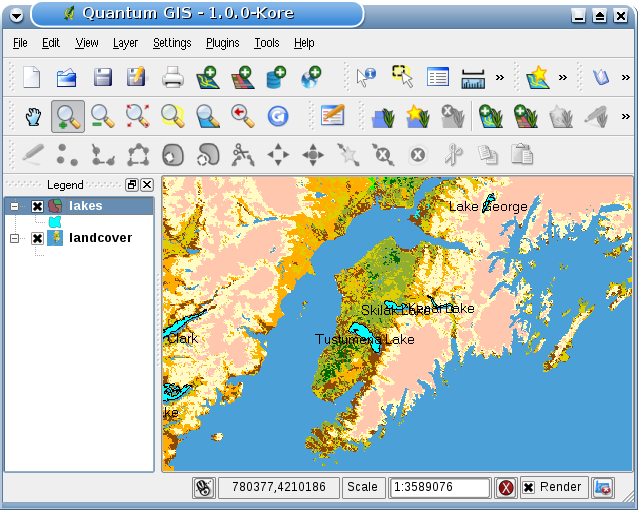
\includegraphics[clip=true, width=12cm]{simple_session}
\end{center}  
\end{figure}

You can see how easy it is to visualize raster and vector layers in 
QGIS. Let's move on to the sections that follow to learn more about the 
available functionality, features and settings and how to use them.

% vim:autoindent:set textwidth=78:

\section{Features at a Glance}\label{feature_glance}

% when the revision of a section has been finalized, 
% comment out the following line:
\updatedisclaimer

After a first and easy sample session in section \ref{label_getstarted} we now 
want to give you a more detailed overview of the existing QGIS functionalities. 
Most features presented in this section will be explained and described in 
own sections later in the manual.

\subsection{Starting and Stopping QGIS}\label{label_startinqgis}

To start QGIS:
\begin{itemize}
\item \nix{assuming that QGIS is installed in the PATH, you can start QGIS 
by typing: \usertext{qgis}  at a command prompt or by double clicking on the QGIS
application link (or shortcut) on the desktop.} 
\item \win{start QGIS using the Start menu or desktop shortcut, 
or double click on a QGIS project file.}
\item \osx{double click the icon in your Applications folder.}
\end{itemize} 

To stop QGIS, click the menu options \{\nix{}\win{File} \osx{QGIS}\} > Quit,
or use the shortcut \keystroke{Ctrl+Q}.
Other ways to exist QGIS include:
\begin{itemize}
\item \nix{type exit in the command window, or 
click on the "x" button  on the upper left corner of the frame.} 
\item \win{click on the red "x" button on the upper left corner of the frame.}
%\item \osx{.}
\end{itemize} 

\subsubsection{Command Line Options}\index{command line options}
\label{label_commandline}

\nix QGIS supports a number of options when started from the command line. To
get a list of the options, enter \usertext{qgis ---help} on the command line.
The usage statement for QGIS is:

\small
\begin{verbatim}
qgis --help
Quantum GIS - 1.0.0 'Kore'
Quantum GIS (QGIS) is a viewer for spatial data sets, including
raster and vector data.
Usage: qgis [options] [FILES]
  options:
        [--snapshot filename]   emit snapshot of loaded datasets to given file
        [--lang language]       use language for interface text
        [--project projectfile] load the given QGIS project
        [--extent xmin,ymin,xmax,ymax]  set initial map extent
        [--help]                this text

  FILES:
    Files specified on the command line can include rasters,
    vectors, and QGIS project files (.qgs):
     1. Rasters - Supported formats include GeoTiff, DEM
        and others supported by GDAL
     2. Vectors - Supported formats include ESRI Shapefiles
        and others supported by OGR and PostgreSQL layers using
        the PostGIS extension
\end{verbatim}
\normalsize

\begin{Tip} \caption{\textsc{Example Using command line arguments}}
\qgistip{You can start QGIS by specifying one or more data files
on the command line. For example, assuming you are in your data directory,
you could start QGIS with two shapefiles and a raster file set to
load on startup using the following command: 
\usertext{qgis ak\_shade.tif alaska.shp majrivers.shp}
}
\end{Tip}

\minisec{Command line option \usertext{---snapshot}}
This option allows you to create a snapshot in PNG format from the current view.
This comes in handy when you have a lot of projects and want to 
generate snapshots from your data.

Currently it generates a PNG-file with 800x600 pixels. A filename can be added after
\usertext{---snapshot}.

\minisec{Command line option \usertext{---lang}}
Based on your locale QGIS, selects the correct localization. If you like to 
change your language, you can provide another language code. E.g.: 
\usertext{---lang=it}
starts QGIS in italian localization. A list of currently supported
languages with language code is provided at
\url{http://wiki.qgis.org/qgiswiki/TranslatorsCorner} 

\minisec{Command line option \usertext{---project}}
Starting QGIS with an existing project file is also possible. Just
add the command line option usertext{--project} followed by your project name
and QGIS will open with all layers loaded described in the given file.

\minisec{Command line option \usertext{---extent}}
To start with a specific map extent use this option. You need to add the bounding
box of your extent in the following order separated by a comma:
\begin{verbatim}
--extent xmin,ymin,xmax,ymax
\end{verbatim}


\subsection{QGIS GUI}\index{main window}
\label{label_qgismainwindow}

When QGIS starts, you are presented with the GUI as shown below
(the numbers 1 through 6 in blue ovals refer to the six major areas of the
interface as discussed below):

\begin{figure}[ht]
   \begin{center}
   \caption{QGIS GUI with Alaska sample data \wincaption}
	 \label{fig:startup}
   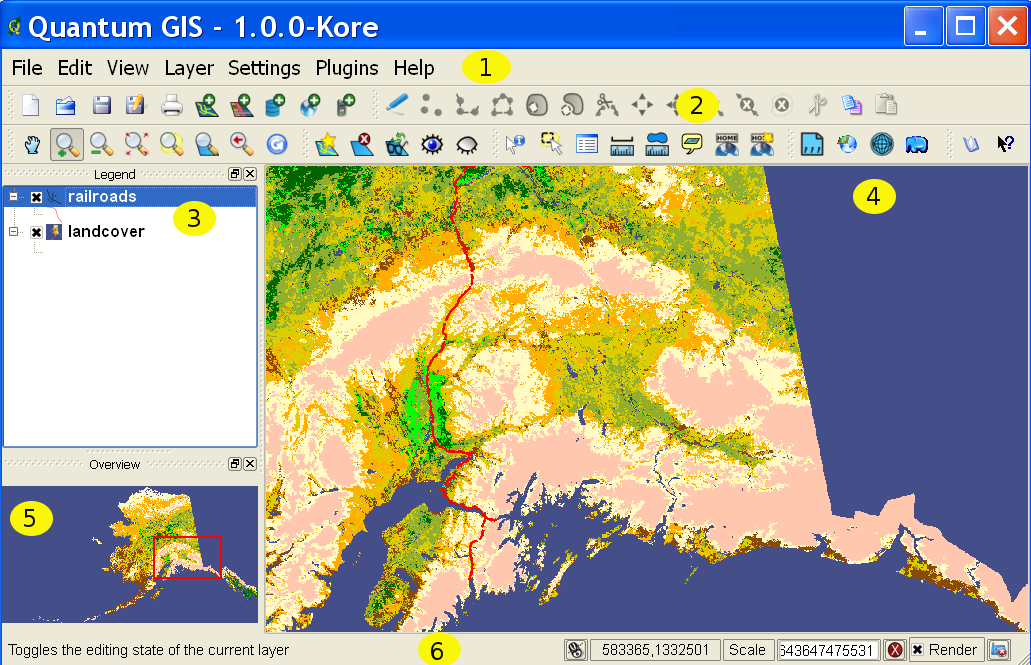
\includegraphics[clip=true, width=17cm]{startup1_0_0}
\end{center} 
\end{figure}

\textbf{Note:} Your window decorations (title bar, etc.) may appear
different depending on your operating system and window manager.

The QGIS GUI is divided into six areas:

\begin{tabbing}
1. Menu Bar \hspace{3cm}\= 4. Map View \\
2. Tool Bar \hspace{3cm}\> 5. Map Overview  \\
3. Map Legend \hspace{3cm}\> 6. Status Bar   
\end{tabbing}

These six components of the QGIS interface are described in more detail in
the following sections.

\subsubsection{Menu Bar}\label{label_menubar}
\index{menus}

The menu bar provides access to various QGIS features using a standard 
hierarchical menu. The top-level menus and a summary of some of the
menu options are listed below, together with the icons of the corresponding 
tools as they appear on the toolbar, as well as keyboard shortcuts.
Although most menu options have a corresponding tool and vice-versa,
the menus are not organized quite like the toolbars. 
The toolbar containing the tool is listed after each menu option as a checkbox
entry. For more information about tools and toolbars, see Section \ref{label_toolbars}.

\begin{tabbing}
\hspace{5.5cm}\=\hspace{3cm}\=\hspace{3.5cm}\= \kill
\hspace{1cm} Menu Option \> Shortcut \> Reference \> Toolbar\\
\end{tabbing}

\begin{itemize}
\item \mainmenuopt{File}
\begin{tabbing}
\hspace{4.5cm}\=\hspace{3cm}\=\hspace{3.5cm}\= \kill
\dropmenuopttwo{mActionFileNew}{New Project}
	\> \keystroke{Ctrl+N}
	\> see Section \ref{sec:projects}
	\> \dropmenucheck{File} \\
\dropmenuopttwo{mActionFileOpen}{Open Project}
	\> \keystroke{Ctrl+O}
	\> see Section \ref{sec:projects}
	\> \dropmenucheck{File} \\
\dropmenuopt{Open Recent Projects}
	\>
	\> see Section \ref{sec:projects} \\
\dropmenuopttwo{mActionFileSave}{Save Project}
	\> \keystroke{Ctrl+S}
	\> see Section \ref{sec:projects}
	\> \dropmenucheck{File} \\
\dropmenuopttwo{mActionFileSaveAs}{Save Project As}
	\> \keystroke{Ctrl+Shift+S}
  \> see Section \ref{sec:projects}
	\> \dropmenucheck{File} \\
\dropmenuopttwo{mActionSaveMapAsImage}{Save as Image}
	\>
	\> see Section \ref{sec:output} \\
%\dropmenuopt{Export to MapServer Map}       - see Section \ref{sec:mapserver_export}
\dropmenuopttwo{mActionFilePrint}{Print Composer}
	\> \keystroke{Ctrl+P}
	\> see Section \ref{label_mapcomposer}
	\> \dropmenucheck{File} \\
\dropmenuopttwo{mActionFileExit}{Exit} 
	\> \keystroke{Ctrl+Q} \\
\end{tabbing}

\item \mainmenuopt{Edit}
\begin{tabbing}
\hspace{4.5cm}\=\hspace{3cm}\=\hspace{3.5cm}\= \kill
\dropmenuopttwo{mActionEditCut}{Cut Features} 
	\> \keystroke{Ctrl+X}
	\> see Section \ref{sec:edit_existing_layer} 
	\> \dropmenucheck{Digitizing} \\
\dropmenuopttwo{mActionEditCopy}{Copy Features}
	\> \keystroke{Ctrl+C}
	\> see Section \ref{sec:edit_existing_layer} 
	\> \dropmenucheck{Digitizing} \\
\dropmenuopttwo{mActionEditPaste}{Paste Features} 
	\> \keystroke{Ctrl+V}
	\> see Section \ref{sec:edit_existing_layer} 
	\> \dropmenucheck{Digitizing} \\
\dropmenuopttwo{mActionCapturePoint}{Capture Point}
	\> \keystroke{.}
	\> see Section \ref{sec:edit_existing_layer} 
	\> \dropmenucheck{Digitizing} \\
\dropmenuopttwo{mActionCaptureLine}{Capture Line}
	\> \keystroke{/}
	\> see Section \ref{sec:edit_existing_layer} 
	\> \dropmenucheck{Digitizing} \\
\dropmenuopttwo{mActionCapturePolygon}{Capture Polygon}
	\> \keystroke{Ctrl+/}
	\> see Section \ref{sec:edit_existing_layer} 
	\> \dropmenucheck{Digitizing} \\
And Other Edit Menu Items
	\>
	\> see Section \ref{sec:edit_existing_layer} 
	\> \dropmenucheck{Digitizing} \\
%\dropmenuopt{Move Feature}
%	\> \> \dropmenucheck{Edit} \\
%\dropmenuopt{Split Features}
%	\> \> \dropmenucheck{Edit} \\
%\dropmenuopt{Delete Selected}
%	\> \> \dropmenucheck{Edit} \\
%\dropmenuopt{Add Vertex}
%	\> \> \dropmenucheck{Edit} \\
%\dropmenuopt{Move Vertex}
%	\> \> \dropmenucheck{Edit} \\
%\dropmenuopt{Delete Vertex}
%	\> \> \dropmenucheck{Edit} \\
%\dropmenuopt{Add Ring}\footnote{New since v0.9} 
%	\>
%	\> \dropmenucheck{Edit} \\
%\dropmenuopt{Add Island} \footnotemark[\value{footnote}] 
%	\>
%	\> \dropmenucheck{Edit} \\
\end{tabbing}


\item \mainmenuopt{View}
\begin{tabbing}
\hspace{4.5cm}\=\hspace{3cm}\=\hspace{3.5cm}\= \kill
\dropmenuopttwo{mActionPan}{Pan Map}
	\>
	\> \> \dropmenucheck{Map Navigation} \\
\dropmenuopttwo{mActionZoomIn}{Zoom In}
	\> \keystroke{Ctrl++}
	\> \> \dropmenucheck{Map Navigation} \\
\dropmenuopttwo{mActionZoomOut}{Zoom Out}
	\> \keystroke{Ctrl+-}
	\> \> \dropmenucheck{Map Navigation} \\
\dropmenuopttwo{mActionSelect}{Select Features}
	\>
	\> \> \dropmenucheck{Attributes} \\
\dropmenuopttwo{mActionIdentify}{Identify Features}
	\> \keystroke{I}
	\> \> \dropmenucheck{Attributes} \\
\dropmenuopttwo{mActionMeasure}{Measure Line}
	\> \keystroke{M}
	\> \> \dropmenucheck{Attributes} \\
\dropmenuopttwo{mActionMeasureArea}{Measure Area}
	\> \keystroke{J}
	\> \> \dropmenucheck{Attributes} \\
\dropmenuopttwo{mActionOpenTable}{Zoom Full}
	\> \keystroke{F}
	\> \> \dropmenucheck{Map Navigation} \\
\dropmenuopttwo{mActionZoomToLayer}{Zoom To Layer}
	\>
	\> \> \dropmenucheck{Map Navigation} \\
\dropmenuopttwo{mActionZoomToSelected}{Zoom To Selection}
	\> \keystroke{Ctrl+J}
	\> \> \dropmenucheck{Map Navigation} \\
\dropmenuopttwo{mActionZoomLast}{Zoom Last}
	\>
	\> \> \dropmenucheck{Map Navigation} \\
\dropmenuopt{Zoom Actual Size}
	\>
	\> \>  \\
\dropmenuopttwo{mActionMapTips}{Map Tips}
	\>
	\> \> \dropmenucheck{Attributes} \\
\dropmenuopttwo{mActionNewBookmark}{New Bookmark}
	\> \keystroke{Ctrl+B}
	\> see Section \ref{sec:bookmarks} 
\> \dropmenucheck{Attributes} \\
\dropmenuopttwo{mActionShowBookmarks}{Show Bookmarks}
	\> \keystroke{B}
	\> see Section \ref{sec:bookmarks} 
	\> \dropmenucheck{Attributes} \\
\dropmenuopttwo{mActionDraw}{Refresh}
	\> \keystroke{Ctrl+R}
	\> \> \dropmenucheck{Map Navigation} \\
\end{tabbing}

\item \mainmenuopt{Layer}
\begin{tabbing}
\hspace{4.5cm}\=\hspace{3cm}\=\hspace{3.5cm}\= \kill
\dropmenuopttwo{mActionNewVectorLayer}{New Vector Layer}
	\> \keystroke{N}
	\>          	
	see Section \ref{sec:create shape}
	\> \dropmenucheck{Manage Layers} \\
\dropmenuopttwo{mActionAddNonDbLayer}{Add a Vector Layer}       
	\> \keystroke{V}
	\>          	
	see Section \ref{label_workingvector}
	\> \dropmenucheck{File} \\
\dropmenuopttwo{mActionAddRasterLayer}{Add a Raster Layer}       
	\> \keystroke{R}
	\>          	
	see Section \ref{label_raster}
	\> \dropmenucheck{File} \\
\dropmenuopttwo{mActionAddLayer}{Add a PostGIS Layer}      
	\> \keystroke{D}
	\>          	
	see Section \ref{label_postgis}
	\> \dropmenucheck{File} \\
\dropmenuopttwo{mActionAddWmsLayer}{Add a WMS Layer}          
	\> \keystroke{W}
	\>          	
	see Section \ref{sec:ogc-wms}
	\> \dropmenucheck{File} \\
\dropmenuopttwo{mActionOpenTable}{Open Attribute Table}
	\> \>
	\> \dropmenucheck{Attributes} \\
\dropmenuopttwo{mActionToggleEditing}{Toggle editing}
	\> \>
	\> \dropmenucheck{Digitizing} \\
\dropmenuopt{Save As Shapefile}
	\\
\dropmenuopt{Save Selection As Shapefile}
	\\
\dropmenuopttwo{mActionRemoveLayer}{Remove Layer}
	\> \keystroke{Ctrl+D}
	\>          	
	\> \dropmenucheck{Manage Layers} \\
\dropmenuopt{Properties}
	\\
\dropmenuopttwo{mActionInOverview}{Add to Overview}
	\> \keystroke{O}
	\>          	
	\> \dropmenucheck{Manage Layers} \\
\dropmenuopttwo{mActionAddAllToOverview}{Add All To Overview}
	\> \keystroke{+}
	\>          	
	\\
\dropmenuopttwo{mActionRemoveAllFromOverview}{Remove All From Overview}
	\> \hspace{1cm}\keystroke{-}
	\>          	
	\\
\dropmenuopttwo{mActionHideAllLayers}{Hide All Layers}
	\> \keystroke{H}
	\>          	
	\> \dropmenucheck{Manage Layers} \\
\dropmenuopttwo{mActionShowAllLayers}{Show All Layers}
	\> \keystroke{S}
	\>          	
	\> \dropmenucheck{Manage Layers} \\
\end{tabbing}

\item \mainmenuopt{Settings}
\begin{tabbing}
\hspace{4.5cm}\=\hspace{3cm}\=\hspace{3.5cm}\= \kill
\dropmenuopttwo{mActionProjectProperties}{Project Properties}  
	\> \keystroke{P}
	\>          	
	see Section \ref{sec:projects}
	\\
\dropmenuopttwo{mActionCustomProjection}{Custom CRS}   
\> \>          	
see Section \ref{sec:customprojections}
	\\
\dropmenuopttwo{mActionOptions}{Options}             
\> \>          	
see Section \ref{subsec:gui_options}
	\\
\end{tabbing}

\item \mainmenuopt{Plugins} - (Futher menu items are added by plugins as they are loaded.)
\begin{tabbing}
\hspace{4.5cm}\=\hspace{3cm}\=\hspace{3.5cm}\= \kill
\dropmenuopttwo{mActionShowPluginManager}{Plugin Manager}          	   
\> \>          	
see Section \ref{sec:managing_plugins}
	\dropmenucheck{Plugins}\\
\end{tabbing}          	

\item \mainmenuopt{Help}
\begin{tabbing}
\hspace{4.5cm}\=\hspace{3cm}\=\hspace{3.5cm}\= \kill
\dropmenuopttwo{mActionHelpContents}{Help Contents}
	\> \keystroke{F1}
	\>           	
	\> \dropmenucheck{Help}\\
\dropmenuopttwo{mActionQgisHomePage}{QGIS Homepage}
	\> \keystroke{Ctrl+H}
	\>          	
	\\
\dropmenuopttwo{mActionCheckQgisVersion}{Check QGIS Version}
	\\
\dropmenuopttwo{mActionHelpAbout}{About}
	\\
\end{tabbing}

\end{itemize}

%See Appendix \ref{app_menu} for complete descriptions of the menu items.

\subsubsection{Toolbars}\label{label_toolbars}
\index{toolbars}

The toolbars provide access to most of the same functions as the menus,
plus additional tools for interacting with the map. Each toolbar item has
popup help available. Hold your mouse over the item and a short description of
the tool's purpose will be displayed. 

Every menubar can be moved around according to your needs. Additionally every
menubar can be switched off using your right mouse button context menu holding
the mouse over the toolbars.

\begin{Tip}
\caption{\textsc{Reappearing toolbars}} \index{layout!toolbars}
\qgistip{If you have accidentally hidden all your toolbars, you can get them back by
choosing menu option \mainmenuopt{View} > \dropmenuopt{Show most toolbars}.}
\end{Tip}

\subsubsection{Map Legend}\label{label_legend}
\index{legend}

% TODO The new legend features need to be described here briefly.
% Marco, would you make a start what is new in the legend?!
The map legend area is used to set the visibility and z-ordering of layers.
Z-ordering means that layers listed nearer the top of the legend are drawn
over layers listed lower down in the legend. The checkbox in each legend
entry can be used to show or hide the layer.\index{layer!visibility}

Layers can be grouped in the legend window by adding a layer group and dragging layers 
into the group. To do so, go with the mouse to the legend window, right click, choose \dropmenuopt{Add group}. 
A new folder appears. Now drag the layers to the folder symbol. It is then possible to toggle the 
visibility of all the layers in the group with one click. To bring layers out of a group, go with 
the mouse to the layer symbol, right click, choose \dropmenuopt{Make to toplevel item}. To give the folder a 
new name, choose \dropmenuopt{Rename} in the right click menu of the group.

The content of the right mouse button context menu depends on if the loaded legend item you hold your 
mouse over is a raster or a vector layer. For GRASS vector layers the \dropmenuopt{toggle editing} is not 
available. See section \ref{grass_digitising} for infos on editing GRASS vector layers. 

\begin{itemize}

\item \textbf{Right mouse button menu for raster layers}
\begin{itemize}
\item \dropmenuopt{Zoom to layer extent}
\item \dropmenuopt{Zoom to best scale (100\%)}
\item \dropmenuopt{Show in overview}
\item \dropmenuopt{Remove}
\item \dropmenuopt{Properties}
\item \dropmenuopt{Rename}
\item \dropmenuopt{Add Group}
\item \dropmenuopt{Expand all}
\item \dropmenuopt{Collapse all}
\item \dropmenuopt{Show file groups}
\end{itemize}

\item \textbf{Right mouse button menu for vector layers}
\begin{itemize}
\item \dropmenuopt{Zoom to layer extent}
\item \dropmenuopt{Show in overview}
\item \dropmenuopt{Remove}
\item \dropmenuopt{Open attribute table}
\item \dropmenuopt{Toggle editing (not available for GRASS layers)}
\item \dropmenuopt{Save as shapefile}
\item \dropmenuopt{Save selection as shapefile}
\item \dropmenuopt{Properties}
\item \dropmenuopt{Rename}
\item \dropmenuopt{Add Group}
\item \dropmenuopt{Expand all}
\item \dropmenuopt{Collapse all}
\item \dropmenuopt{Show file groups}
\end{itemize}

\item \textbf{Right mouse button menu for layer groups} 
\begin{itemize}
\item \dropmenuopt{Remove}
\item \dropmenuopt{Rename}
\item \dropmenuopt{Add Group}
\item \dropmenuopt{Expand all}
\item \dropmenuopt{Collapse all}
\item \dropmenuopt{Show file groups}
\end{itemize}

\end{itemize}

If several vector data sources have the same vector type and the same attributes, their 
symbolisations may be grouped. This means that if the symbolisation of one data source is 
changed, the others automatically have the new symbolisation as well. To group symbologies, open 
the right click menu in the legend window and choose \dropmenuopt{Show file groups}. The file groups of the 
layers appear. It is now possible to drag a file from one file group into another one. If this is done, 
the symbologies are grouped. Note that QGIS only permits the drag if the two layers are able to share 
symbology (same vector type and same attributes).  

%% isn't included in Titan anymore, except for an "toggle overview"
%Each legend entry can show the following mini icons:
%
%
\includegraphics[width=0.7cm]{pyramid} This is a raster
%that has pyramids built for it to improve rendering efficiency (see
%Section \ref{raster_pyramids}).\\
%
\includegraphics[width=0.7cm]{no_pyramid} This is a
%raster that has no pyramid layers (see Section \ref{raster_pyramids}).\\
%
\includegraphics[width=0.7cm]{inoverview} This layer is
%shown in the overview map area as well as in the main map window.\\
%\includegraphics[width=0.7cm]{editable} This is a vector
%layer that is currently enabled for editing.\\

\subsubsection{Map View}\label{label_mapview}
\index{map!view}

This is the 'business end' of QGIS - maps are displayed in this area! The
map displayed in this window will depend on the vector and raster layers you
have chosen to load (see sections that follow for more information on how to
load layers). The map view can be panned (shifting the focus of the map display
to another region) and zoomed in and out. Various other operations can be
performed on the map as described in the toolbar description above.  The map
view and the legend are tightly bound to each other - the maps in view reflect
changes you make in the legend area.  

\begin{Tip}\caption{\textsc{Zooming the Map with the Mouse
Wheel}}\index{zoom!mouse wheel}
\qgistip{You can use the mouse wheel to zoom in and out on the map. Place
the mouse cursor inside the map area and roll it forward (away from you) to
zoom in and backwards (towards you) to zoom out. The mouse cursor is the 
center where the zoom occurs. You can customize the behavior of the mouse
wheel zoom using the \tab{Map tools} tab under the \mainmenuopt{Settings} >\dropmenuopt{Options} menu.  }
\end{Tip}

\subsubsection{Map Overview}\label{label_mapoverview}
\index{map!overview}

The map overview area provides a full extent view of layers added to it.
Within the view is a rectangle showing the current map extent. This allows
you to quickly determine which area of the map you are currently viewing. Note
that labels are not rendered to the map overview even if the layers in the
map overview have been set up for labeling. 
You can add a single layer to the
overview by right-clicking on it in the legend and choosing \dropmenuopt{Show in overview}. You can also add or remove all layers to the overview using the
Overview tools on the toolbar.

You can also grab the red rectangle showing your current extent and pan around; the
map view will update accordingly.

\subsubsection{Status Bar}\label{label_statusbar}

The status bar shows you your current position in map coordinates (e.g.
meters or decimal degrees) as the mouse pointer is moved across the map view.
The status bar also shows the view extents of the map view as you pan and
zoom in and out. A progress bar in the status bar shows progress of rendering
as each layer is drawn to the map view. In some cases, such as the gathering
of statistics in raster layers, the progress bar will be used to show the
status of lengthy operations. On the right side of the status bar is a small
checkbox which can be used to temporarily prevent layers being rendered to the
map view (see Section \ref{subsec:redraw_events} below). At the far right of
the status bar is a projector icon. Clicking on this opens the projection
properties for the current project.

\subsection{Rendering}\label{subsec:redraw_events}\index{rendering}

By default, QGIS renders all visible layers whenever the map canvas must be
refreshed. The events that trigger a refresh of the map canvas include:

\begin{itemize}
\item Adding a layer
\item Panning or zooming
\item Resizing the QGIS window
\item Changing the visibility of a layer or layers
\end{itemize}

QGIS allows you to control the rendering process in a number of ways.

\subsubsection{Scale Dependent Rendering}\index{rendering!scale dependent}
\label{label_scaledepend}

Scale dependent rendering allows you to specify the minimum and maximum
scales at which a layer will be visible.  To set scale dependency rendering,
open the \dialog{Properties} dialog by double-clicking on the layer in the legend. On
the \tab{General} tab, set the minimum and maximum scale values and then
click on the \checkbox{Use scale dependent rendering} checkbox.

You can determine the scale values by first zooming to the level you want
to use and noting the scale value in the QGIS status bar.\index{scale}

\subsubsection{Controlling Map Rendering}\label{label_controlmap}

Map rendering can be controlled in the following ways:

\minisec{Suspending Rendering}\index{rendering!suspending}
\label{label_suspendrender}

To suspend rendering, click the \checkbox{Render} checkbox in the lower right
corner of the statusbar. When the \checkbox{Render} box is not checked, QGIS
does not redraw the canvas in response to any of the events described in
Section \ref{subsec:redraw_events}. Examples of when you might want to suspend
rendering include:

\begin{itemize}
\item Add many layers and symbolize them prior to drawing
\item Add one or more large layers and set scale dependency before drawing
\item Add one or more large layers and zoom to a specific view before
drawing
\item Any combination of the above
\end{itemize}

Checking the \checkbox{Render} box enables rendering and causes and immediate
refresh of the map canvas.

\minisec{Setting Layer Add Option}\label{label_settinglayer}
\index{rendering!options}\index{layers!initial visibility}

You can set an option to always load new layers without drawing them. This
means the layer will be added to the map, but its visibility checkbox in the
legend will be unchecked by default. To set this option, choose
menu option \mainmenuopt{Settings} > \dropmenuopt{Options} and click on the
\tab{Rendering} tab. Uncheck the \checkbox{By default new layers added to the map 
should be
displayed} checkbox. Any layer added to the map will be off (invisible) by
default.

%\minisec{Stopping Rendering}\index{rendering!halting}
%\label{label_stoprender}
%
%To stop the map drawing, press the ESC key. This will halt the refresh of
%the map canvas and leave the map partially drawn. It may take a bit of time
%between pressing ESC and the time the map drawing is halted.
%
%\textbf{NOTE}: It is currently not possible to stop rendering - this was disabled 
%in qt4 port because of User Interface (UI) problems and crashes.

\minisec{Updating the Map Display During Rendering}
\label{label_updatemap}\index{rendering!update during drawing}

You can set an option to update the map display as features are drawn. By
default, QGIS does not display any features for a layer until the entire
layer has been rendered. To update the display as features are read from the
datastore, choose menu option \mainmenuopt{Settings} > \dropmenuopt{Options}
click on the \tab{Rendering} tab. Set the feature count to an
appropriate value to update the display during rendering. Setting a value of 0
disables update during drawing (this is the default). Setting a value too low
will result in poor performance as the map canvas is continually updated
during the reading of the features. A suggested value to start with is 500. 

\subsection{Measuring}\label{sec:measure}\index{measure}

Measuring works within projected coordinate systems only (e.g., UTM). If 
the loaded map is defined with a geographic coordinate system
(latitude/longitude), the results from line or area measurements will be 
incorrect. To fix this you need to set an appropriate map coordinate system.

\subsubsection{Measure length}\index{measure:line length}

\includegraphics[width=0.7cm]{mActionMeasure} 
QGIS is also able to measure real distances between given 
points according to a defined ellipsoid. Therefore choose menu option \mainmenuopt{Settings} > \dropmenuopt{Options}, 
click on the \tab{Map tools} tab and choose the appropriate ellipsoid. The tool then allows you to 
click points on the map. Each segment-length shows up in the measure-window and additionaly the total 
length is printed. To stop measuring click your right mouse button. 

\subsubsection{Measure areas}\index{measure:areas}

\includegraphics[width=0.7cm]{mActionMeasureArea} 
Also areas can be measured. The window only shows the
accumulated area-size in the measure window 

% measure-tools side by side
\begin{figure}[h]
\caption{Measure tools in action} \label{fig:measure}
\centering
   \subfigure[Measure lines] {\label{subfig:measure_line}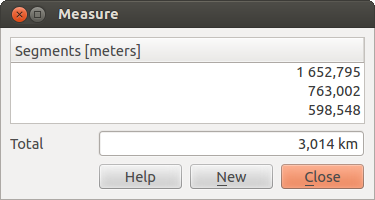
\includegraphics[clip=true, width=0.4\textwidth]{measure_line}}\goodgap
   \subfigure[Measure areas]{\label{subfig:measure_area}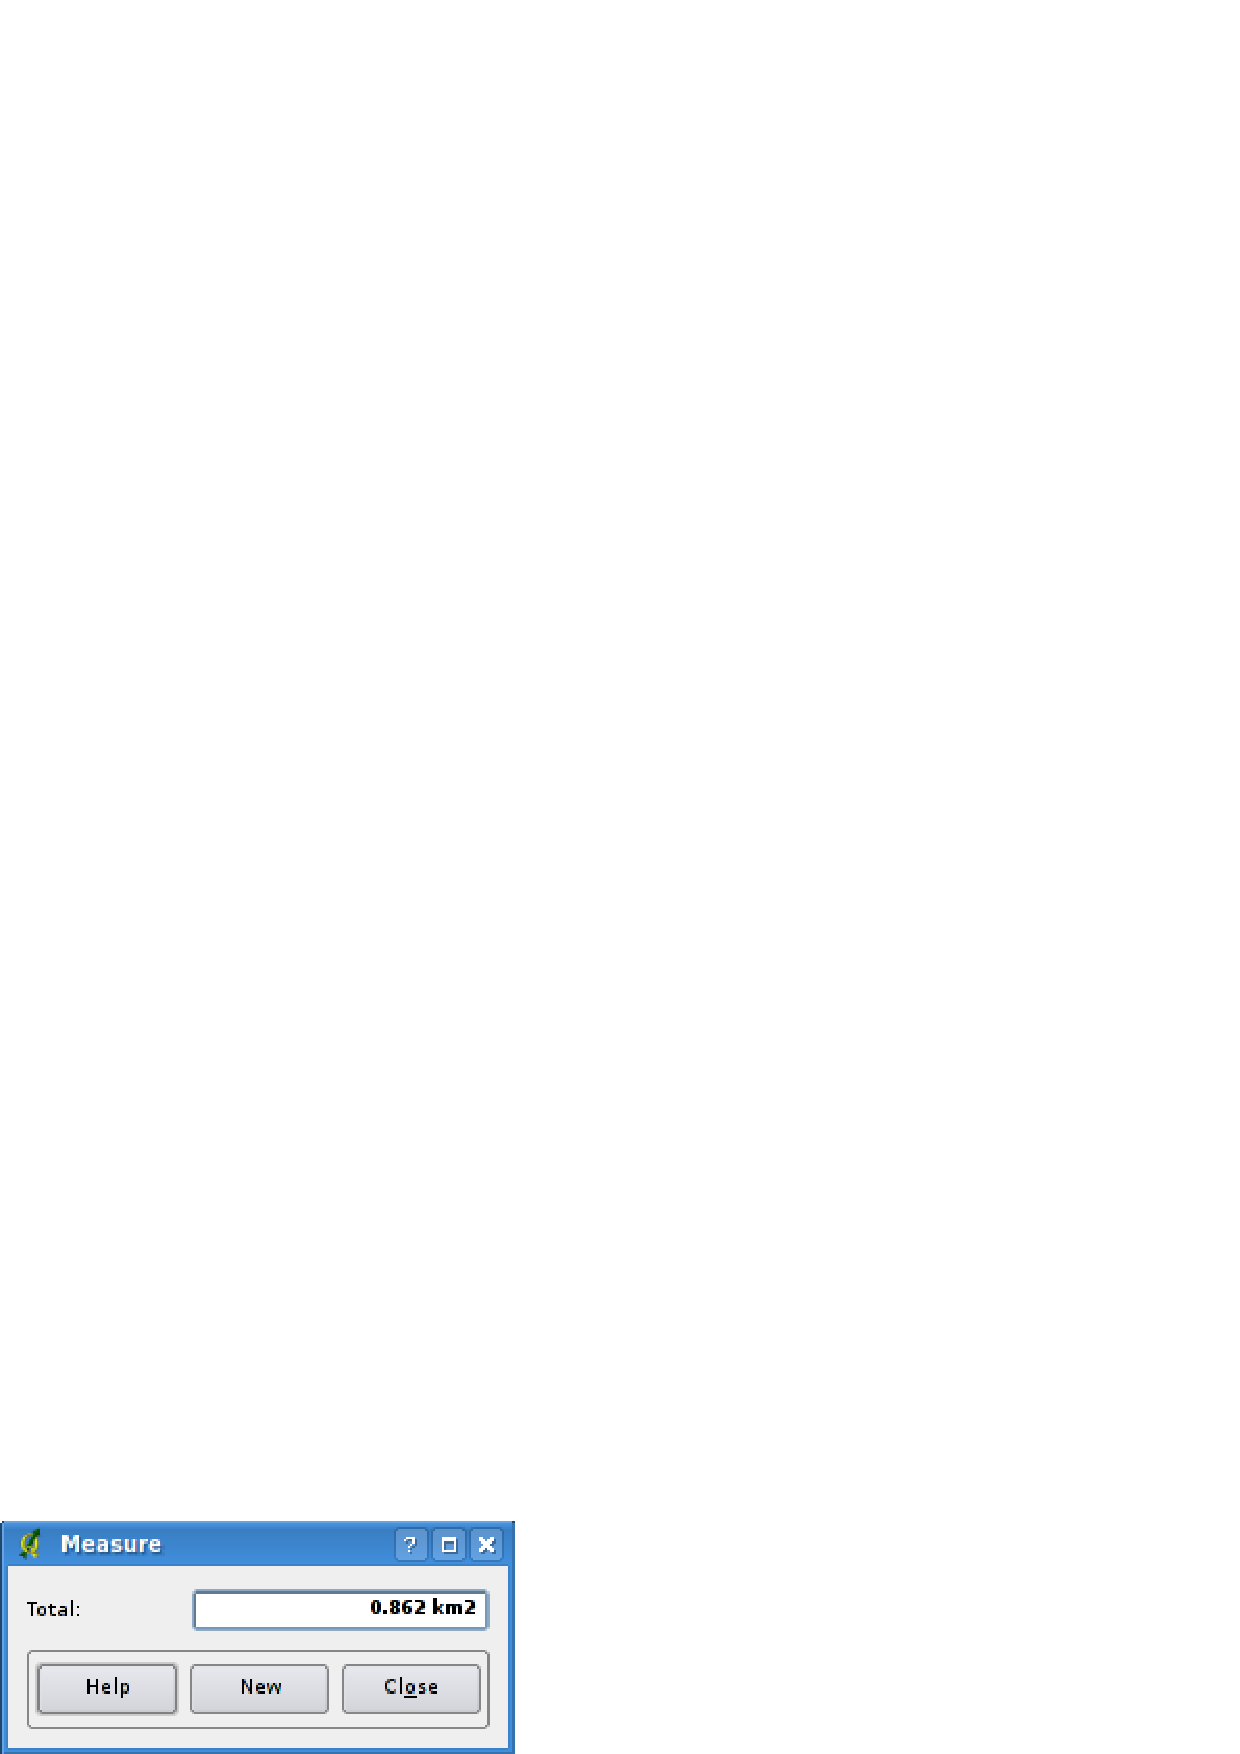
\includegraphics[clip=true, width=0.4\textwidth]{measure_area}}
\end{figure}

\subsection{Projects}\label{sec:projects}\index{projects}

The state of your QGIS session is considered a Project.  QGIS
works on one project at a time.  Settings are either considered
as being per-project, or as a default for new projects (see
Section \ref{subsec:gui_options}).

QGIS can save the state of your workspace into a project file using
the menu options 
\mainmenuopt{File} > \dropmenuopttwo{mActionFileSave}{Save Project}
or \mainmenuopt{File} > \dropmenuopttwo{mActionFileSaveAs}{Save Project As}.

Load saved projects into a QGIS session using 
\mainmenuopt{File} > \dropmenuopttwo{mActionFileOpen}{Open Project}
or \mainmenuopt{File} > \dropmenuopt{Open Recent Project}.
If you wish to clear your session and start fresh, choose
\mainmenuopt{File} > \dropmenuopttwo{mActionFileNew}{New Project}.
Either of these menu options will prompt you to save the existing project
if changes have been made since it was opened or last saved.

The kinds of information saved in a project file include:

\begin{itemize}
\item Layers added
\item Layer properties, including symbolization
\item Projection for the map view
\item Last viewed extent
\end{itemize}

The project file is saved in XML format, so it is possible to edit
the file outside QGIS if you know what you are doing.  

The file format was updated several times compared to earlier QGIS versions. Project files 
from older QGIS versions may not work properly anymore.

\subsection{Output}\label{sec:output}\index{output!save as image!print composer!quick print}
There are several ways to generate output from your QGIS session.
We have discussed one already in Section \ref{sec:projects}---
saving as a project file. Here is a sampling of other ways to produce output files:
\begin{itemize}
\item Menu option \dropmenuopttwo{mActionSaveMapAsImage}{Save as Image} opens a
file dialog where you select the name, path and type of image (PNG or JPG format).
\end{itemize}


\subsection{GUI Options}
\label{subsec:gui_options}

\includegraphics[width=0.7cm,clip=true]{mActionOptions} 
Some basic options for QGIS
can be selected using the \dialog{Options} dialog. Select the 
menu option \mainmenuopt{Settings} >
 \dropmenuopttwo{mActionOptions}{Options} or press \keystroke{Alt-O}. The tabs where you can 
optmize your options are:

\minisec{General Tab}

\begin{itemize}
\item Ask to save project changes when required
\end{itemize}

\minisec{Appearance Tab}

\begin{itemize}
\item Hide or show splash screen at startup
\item Change the icon theme 
\item Change Selection and backgroud Color
\item Make layer names appear with Capitals
\end{itemize}

\minisec{Rendering Tab}

\begin{itemize}
\item Update features during drawing or not until all features have been read.
\item Set new layer visible or unvisible when loaded 
\item Make lines appear less jagged at the expense of some drawing performance
\item Fix problems with incorrectly filled polygons
\item Continously redraw when dragging the legend/map divider 
\end{itemize}

\minisec{Map tools Tab}

\begin{itemize}
\item Define Search Radius as a percentage of the map width
\item Define Ellipsoid for distance calculations
\item Set Rubberband Color for Measure Tool
\item Define Mouse wheel action (Zoom, Zoom and recenter, Nothing)
\item Set Zoom factor for wheel mouse
\end{itemize}

\minisec{Projection Tab}

\begin{itemize}
\item Define what to do, when a layer is loaded without projection information
\begin{itemize}
\item Prompt for projection
\item Project wide default projection will be used
\item Global default projection displayed below will be used
\end{itemize}
\end{itemize}

\minisec{Locale Tab}

\begin{itemize}
\item Overwrite system locale and use defined locale instead
\item Information about active system locale
\end{itemize}

\minisec{Help Browser Tab}

\begin{itemize}
\item Define Browser to display help documents
\end{itemize}


You can modify the options according to your needs. Some of the changes may 
require a restart of QGIS before they will be effective.

\begin{itemize}
\item \nix{everything is saved in:}
\begin{verbatim}
$HOME/.config/QuantumGIS/qgis.conf
\end{verbatim}
This is a normal text file consisting of blocks, where QGIS saves its current
display options, PostGIS and WMS connections, and other settings.

\item \win{settings are stored in the registry under:}
\begin{verbatim}
\\HKEY_CURRENT_USER\Software\QuantumGIS\qgis
\end{verbatim}

\item \osx{you can find your settings in:}
\begin{verbatim}
$HOME/Library/Preferences/org.qgis.qgis.plist
\end{verbatim}
\end{itemize}


\subsection{Spatial Bookmarks}\label{sec:bookmarks}
\index{bookmarks}
\index{spatial bookmarks|\see{bookmarks}}

Spatial Bookmarks allow you to ``bookmark'' a geographic location and return to it later.

\subsubsection{Creating a Bookmark}
To create a bookmark:
\begin{enumerate}
\item Zoom or pan to the area of interest.
\item Select the menu option \mainmenuopt{View} > \dropmenuopt{New Bookmark} or press \keystroke{Ctrl-B}.
\item Enter a descriptive name for the bookmark (up to 255 characters).
\item Click \button{OK} to add the bookmark or \button{Cancel} to exit without adding the bookmark.
\end{enumerate}

Note that you can have multiple bookmarks with the same name.

\subsubsection{Working with Bookmarks}
To use or manage bookmarks, select the menu 
option \mainmenuopt{View} > \dropmenuopt{Show Bookmarks}.
The \dialog{Geospatial Bookmarks} dialog allows you to zoom to or delete a bookmark.
You can not edit the bookmark name or coordinates.

\subsubsection{Zooming to a Bookmark}
From the \dialog{Geospatial Bookmarks} dialog, select the desired bookmark by clicking on it, 
then click \button{Zoom To}.
You can also zoom to a bookmark by double-clicking on it.

\subsubsection{Deleting a Bookmark}
To delete a bookmark from the \dialog{Geospatial Bookmarks} dialog, click on it then click
 \button{Delete}.
Confirm your choice by clicking \button{Yes} or cancel the delete by clicking \button{No}.

% vim:autoindent:set textwidth=78:

\section{Working with Vector Data}\label{label_workingvector}
\index{vector layers|(}

% when the revision of a section has been finalized,
% comment out the following line:
% \updatedisclaimer


QGIS supports vector data in a number of formats, including those
supported by the OGR library data provider plugin, such as ESRI shapefiles,
\index{shapefiles}\index{ESRI!shapefiles}\index{SHP files}
MapInfo MIF (interchange format)\index{MIF files}\index{MapInfo!MIF files}
and MapInfo TAB (native format).\index{TAB files}\index{MapInfo!TAB files}
You find a list of OGR supported vector formats in Appendix~\ref{appdx_ogr}.

QGIS also supports PostGIS\index{PostGIS}\index{PostgreSQL!PostGIS} layers 
in a PostgreSQL database using the PostgreSQL data provider plugin.
Support for additional data types (eg. delimited text) is provided by 
additional data provider plugins.\index{delimited text}

This section describes how to work with two common formats:
ESRI shapefiles and PostGIS layers. Many of the
features available in QGIS work the same regardless of the vector data source.
This is by design and includes the identify, select, labeling and attributes
functions.

Working with GRASS vector data is described in Section \ref{sec:grass}.

\subsection{ESRI Shapefiles}
\index{vector layers!ESRI shapefiles}
\index{shapefiles}
\index{ESRI!shapefiles}
\index{SHP files}

The standard vector file format used in QGIS is the ESRI Shapefile. It's support 
is provided by the OGR Simple Feature Library (\url{http://www.gdal.org/ogr/})
\index{OGR}. A shapefile actually consists of a minimum of three files:
\index{shapefile!format}

\begin{itemize}
\item \filename{.shp} file containing the feature geometries.
\item \filename{.dbf} file containing the attributes in dBase format.
\item \filename{.shx} index file.
\end{itemize}

Ideally it comes with another file with a \filename{.prj} suffix, that contains
the projection information for the shapefile. There can be more files belonging 
to a shapefile dataset. To have a closer look at this we recommend the technical 
specification for the shapefile format, that can be found at \url{http://www.esri.com/library/whitepapers/pdfs/shapefile.pdf}.
\index{shapefile!specification}.

\subsubsection{Loading a Shapefile}\label{sec:load_shapefile}

\includegraphics[width=0.7cm]{mActionAddNonDbLayer} 
To load a shapefile, start
QGIS and click on the \toolbtntwo{mActionAddNonDbLayer}{Add a vector layer}
toolbar button\index{shapefile!loading} or simply type \keystroke{V}. This same tool can be used to
load any of the formats supported by the OGR library.

Clicking on the tool brings up a standard open file dialog (see Figure
\ref{fig:openshapefile}) which allows you to navigate the file system and load
a shapefile or other supported data source. 
The selection box \selectstring{Files of type}{\ldots} allows you to preselect some OGR supported file formats.

You can also select the Encoding type for the shapefile if desired.

\begin{figure}[ht]
   \begin{center}
   \caption{Open an OGR Supported Vector Layer Dialog \nixcaption}\label{fig:openshapefile}\smallskip
   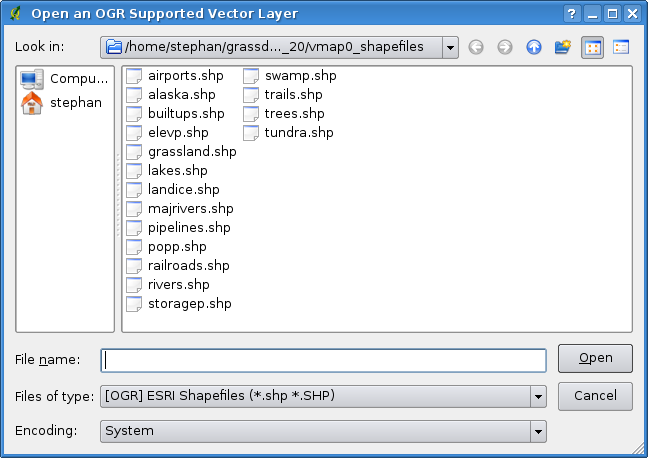
\includegraphics[clip=true, width=14cm]{shapefileopendialog}
\end{center} 
\end{figure}

Selecting a shapefile from the list and clicking \button{Open} loads it into QGIS. Figure
\ref{fig:loadedshapefile} shows QGIS after loading the \filename{alaska.shp} file.

\begin{figure}[ht]
   \begin{center}
   \caption{QGIS with Shapefile of Alaska loaded \nixcaption}\label{fig:loadedshapefile}\smallskip
   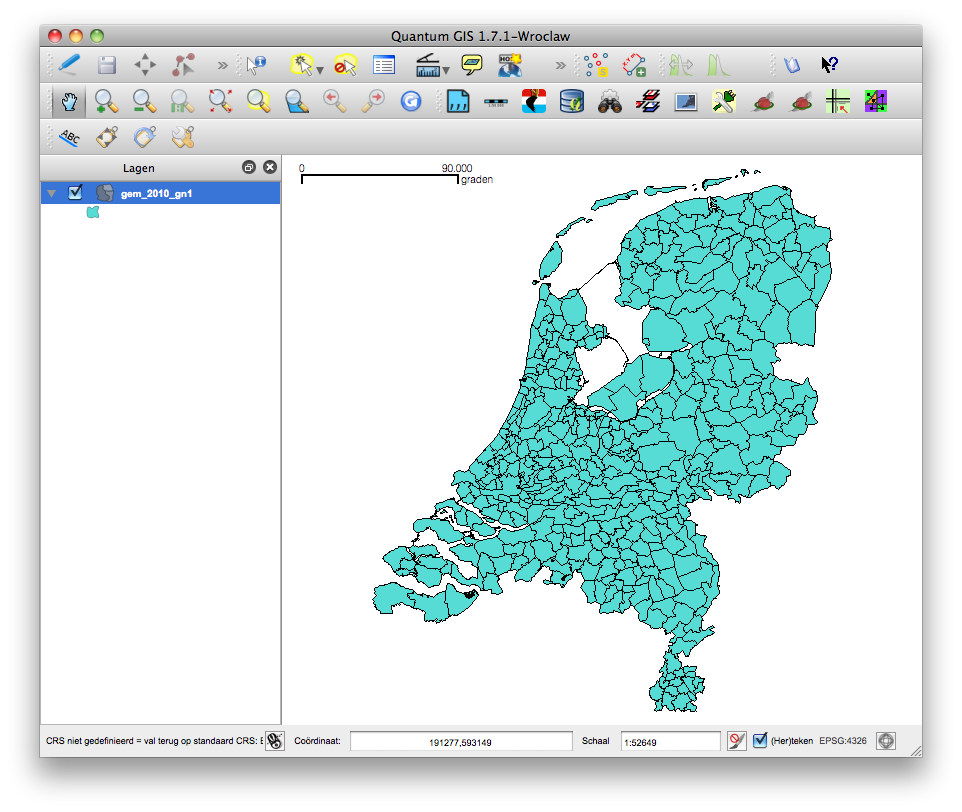
\includegraphics[clip=true, width=16cm]{shapefileloaded}
\end{center} 
\end{figure}

\begin{Tip}\caption{\textsc{Layer Colors}}
\qgistip{When you add a layer to the map, it is assigned a random color. When
adding more than one layer at a time, different colors are assigned to each layer. }
\end{Tip}

Once loaded, you can zoom around the shapefile using the map navigation tools.
To change the symbology of a layer, open the \dialog{Layer Properties} dialog by double
clicking on the layer name or by right-clicking on the name in the legend and
choosing \dropmenuopt{Properties} from the popup menu. See
Section \ref{sec:symbology} for more information on setting symbology of
vector layers.
  
\subsubsection{Improving Performance}

To improve the performance of drawing a shapefile, you can create a spatial
index. A \index{spatial index!shapefiles} spatial index will improve the 
speed of both zooming and panning. Spatial indexes used by QGIS have a 
\filename{.qix} extension.

Use these steps to create the index:

\begin{itemize}
\item Load a shapefile.
\item Open the \dialog{Layer Properties} dialog by double-clicking on the
shapefile name in the legend or by right-clicking and choosing
\dropmenuopt{Properties} from the popup menu.
\item In the tab \tab{General} click the \button{Create Spatial Index} button.
\end{itemize}

\subsubsection{Loading a MapInfo Layer}
\index{vector layers!MapInfo}

To load a MapInfo layer, click on the 
\toolbtntwo{mActionAddNonDbLayer}{Add a vector layer}
toolbar bar button or type \keystroke{V}, change the file type filter to
\selectstring{Files of Type}{[OGR] MapInfo (*.mif
*.tab *.MIF *.TAB)} and select the layer you want to load.

\subsubsection{Loading an ArcInfo Coverage}
\index{vector layers!ArcInfo Coverage}

Loading an ArcInfo coverage is done using the same method as with a
shapefiles and MapInfo layers. Click on the 
\toolbtntwo{mActionAddNonDbLayer}{Add a vector layer}
toolbar button or type \keystroke{V} to open the 
\dialog{Open on OGR Supported Vector Layer} 
dialog and change the file type filter to
\selectstring{Files of Type}{All files (*.*)}. Navigate to the coverage directory and select one
of the following files (if present in your coverage):

\begin{itemize}
\item \filename{.lab} - to load a label layer (polygon labels or standing points).
\item \filename{.cnt} - to load a polygon centroid layer 
\item \filename{.arc} - to load an arc (line) layer.
\item \filename{.pal} - to load a polygon layer.
\end{itemize}

\subsection{PostGIS Layers}
\index{vector layers!PostGIS|see{PostGIS}}
\index{PostGIS!layers}
\label{label_postgis} 

PostGIS layers are stored in a PostgreSQL database. The advantages of PostGIS
are the spatial indexing, filtering and query capabilities it provides. Using PostGIS,
vector functions such as select and identify work more accurately than with
OGR layers in QGIS.

To use PostGIS layers you must:\index{PostgreSQL!loading layers}

\begin{itemize}
\item Create a stored connection in QGIS to the PostgreSQL database (if one is
not already defined).\index{PostgreSQL!connection}
\item Connect to the database.
\item Select the layer to add to the map.
\item Optionally provide a SQL \usertext{where}
clause to define which features
to load from the layer.
\item Load the layer.
\end{itemize}

\subsubsection{Creating a stored
Connection}\index{PostgreSQL!connection}\label{sec:postgis_stored}


\includegraphics[width=0.7cm]{mActionAddLayer} The first time
you use a PostGIS data source, you must create a connection to the PostgreSQL
database that contains the data. Begin by clicking on the
\toolbtntwo{mActionAddLayer}{Add a PostGIS Layer} toolbar button, selecting the
\dropmenuopttwo{mActionAddLayer}{Add a PostGIS Layer...} option from the \mainmenuopt{Layer} menu or typing
\keystroke{D}. 
The \dialog{Add PostGIS Table(s)} dialog will
be displayed. To access the connection manager\index{PostgreSQL!connection
manager}, click on the \button{New} button to display the \dialog{Create a New
PostGIS Connection} dialog. The parameters required for a connection are shown
in table \ref{tab:postgis_connection_parms}.

\begin{table}[ht]\index{PostgreSQL!connection parameters}
\centering
\caption{PostGIS Connection
Parameters}\label{tab:postgis_connection_parms}\medskip
 \begin{tabular}{|l|p{5in}|}
\hline Name & A name for this connection. Can be the same as \textsl{Database}.
\\
\hline Host \index{PostgreSQL!host}
& Name of the database host. This must be a resolvable host name the same as
would be used to open a telnet connection or ping the host. If the database is 
on the same computer as QGIS, simply enter 'localhost' here. \\
\hline Database \index{PostgreSQL!database} & Name of the database.  \\
\hline Port \index{PostgreSQL!port}& Port number the PostgreSQL database
server listens on. The default port is 5432.\\
\hline Username \index{PostgreSQL!username}& User name used to login to the
database. \\
\hline Password \index{PostgreSQL!password}& Password used with
\textsl{Username} to connect to the database.\\
\hline
\end{tabular}
\end{table}

Optional you can activate follwing checkboxes:

\begin{itemize}
\item \checkbox{Save Password}
\item \checkbox{Only look in the geometry\_columns table}
\item \checkbox{Only look in the 'public' schema}
\end{itemize}

Once all parameters and options are set, you can test the connection by
clicking on the \button{Test Connect} button\index{PostgreSQL!connection!testing}.

\begin{Tip}\caption{\textsc{QGIS User Settings and
Security}}\index{settings}\index{security}
\qgistip{Your customized settings for QGIS are stored based on the operating
system. \nix, the settings are stored in your home directory in
\filename{.qt/qgisrc}. \win, the settings are stored in the registry. Depending on
your computing environment, storing passwords in your QGIS settings may be a
security risk.
}
\end{Tip}

\subsubsection{Loading a PostGIS Layer}\index{PostgreSQL!loading layers}


\includegraphics[width=0.7cm]{mActionAddLayer} Once you have one or more
connections defined, you can load layers from the PostgreSQL database. Of
course this requires having data in PostgreSQL. See Section
\ref{sec:loading_postgis_data} for a discussion on importing data into the
database. 

To load a layer from PostGIS, perform the following steps:

\begin{itemize}
\item If the \dialog{Add PostGIS Table(s)} dialog is not already open, click on the
\toolbtntwo{mActionAddLayer}{Add a PostGIS Layer} toolbar button.
\item Choose the connection from the drop-down list and click \button{Connect}.
\item Find the layer you wish to add in the list of available layers.
\item Select it by clicking on it. You can select multiple layers by holding
down the \keystroke{shift} key while clicking. See Section \ref{sec:query_builder} for
information on using the PostgreSQL Query Builder to further define the layer.
\item Click on the \button{Add} button to add the layer to the map.
\end{itemize}

\begin{Tip}\caption{\textsc{PostGIS Layers}}
\qgistip{Normally a PostGIS layer is defined by an entry in the
geometry\_columns table. From version \OLD % should be 0.9.0 
on, QGIS can load layers that do not have
an entry in the geometry\_columns table. This includes both tables and views.
Defining a spatial view provides a powerful means to visualize your data. Refer
to your PostgreSQL manual for information on creating views.}
\end{Tip}

\subsubsection{Some details about PostgreSQL
layers}\label{sec:postgis_details}
\index{PostgreSQL!layer details}

This section contains some details on how QGIS accesses PostgreSQL
layers. Most of the time QGIS should simply provide you with a list of
database tables that can be loaded, and load them on request. However,
if you have trouble loading a PostgreSQL table into QGIS, the information
below may help you understand any QGIS messages and give you direction on
changing the PostgreSQL table or view definition to allow QGIS to load it.

QGIS requires that PostgreSQL layers contain a column that can be
used as a unique key for the layer. For tables this usually means
that the table needs a primary key, or a column with a unique
constraint on it. QGIS additionally requires that this column be of
type int4 (an integer of size 4 bytes). If a table lacks these items,
the oid column will be used instead. Performance will be improved if the
column is indexed (note that primary keys are automatically indexed in
PostgreSQL). 

If the PostgreSQL layer is a view, the same requirements exists, but
views don't have primary keys or columns with unique constraints on
them. In this case QGIS will try to find a column in the view that is
derived from a table column that is suitable. If one cannot be found,
QGIS will not load the layer. If this occurs, the solution is to alter
the view so that it does include a suitable column (a type of int4
and either a primary key or with a unique constraint, preferably indexed).

\subsubsection{Importing Data into PostgreSQL}\label{sec:loading_postgis_data}
\index{PostGIS!SPIT!importing data}

\minisec{shp2pgsql}
Data can be imported into PostgreSQL using a number of methods. PostGIS
includes a utility called \filename{shp2pgsql} that can be used to import shapefiles into
a PostGIS enabled database. For example, to import a shapefile named
\filename{lakes.shp}
into a PostgreSQL database named \usertext{gis\_data}, use the following command:

\begin{verbatim} 
  shp2pgsql -s 2964 lakes.shp lakes_new | psql gis_data
\end{verbatim}

This creates a new layer named \usertext{lakes\_new} in the
\usertext{gis\_data} database. The
new layer will have a spatial reference identifier (SRID) of 2964. See Section 
\ref{label_projections} for more information on spatial reference systems and
projections.
\begin{Tip}
\caption{\textsc{Exporting datasets from PostGIS}\index{PostGIS!Exporting}}
\qgistip{Like the import-tool \filename{shp2pgsql} there is also a tool to export
PostGIS-datasets as shapefiles: \filename{pgsql2shp}. This is shipped within your
PostGIS distribution.} 
\end{Tip}

\minisec{SPIT Plugin}

\includegraphics[width=0.7cm]{spiticon} QGIS comes with a
plugin named 
SPIT (Shapefile to PostGIS Import Tool)\index{PostGIS!SPIT}.
SPIT can be used to load multiple shapefiles at one time and includes support
for schemas. To use SPIT, open the Plugin Manager from the \mainmenuopt{Plugins}
menu, check the box next to the \checkbox{SPIT plugin} and click \button{OK}. The SPIT
icon will be added to the plugin toolbar\index{PostGIS!SPIT!loading}. 

To import a shapefile, click on the \toolbtntwo{spiticon}{SPIT} tool in the 
toolbar to open the 
\dialog{SPIT - Shapefile to PostGIS Import Tool} dialog. Select the PostGIS database 
you want to connect to and click on \button{Connect}. Now you can add one or more 
files to the queue by clicking on the \button{Add} button. To process the files, 
click on the \button{OK} button. The progress of the import as well as any 
errors/warnings will be displayed as each shapefile is processed.

\begin{Tip}\caption{\textsc{Importing Shapefiles Containing
PostgreSQL Reserved Words}}\index{PostGIS!SPIT!reserved words}
\qgistip{If a shapefile is added to the queue containing fields that are
reserved words in the PostgreSQL database a dialog will popup showing the
status
of each field. You can edit the field names\index{PostGIS!SPIT!editing field names}
prior to import and change any that are reserved words (or change any other
field names as desired). Attempting to
import a shapefile with reserved words as field names will likely fail.}
\end{Tip} 

\minisec{ogr2ogr}
Beside \filename{shp2pgsql} and \filename{SPIT} there is another tool for feeding
geodata in PostGIS: \filename{ogr2ogr}. This is part of your GDAL installation.
To import a shapefile into PostGIS, do the following:
\begin{verbatim}
  ogr2ogr -f "PostgreSQL" PG:"dbname=postgis host=myhost.de user=postgres \
  password=topsecret" alaska.shp
\end{verbatim}

This will import the shapefile \filename{alaska.shp} into the PostGIS-database
\usertext{postgis}
using the user \usertext{postgres} with the password \usertext{topsecret} on host
\server{myhost.de}.

Note that OGR must be built with PostgreSQL to support PostGIS.
You can see this by typing
\begin{verbatim}
ogrinfo --formats | grep -i post
\end{verbatim}

If you like to use PostgreSQL's \filename{COPY}-command instead of the default
\filename{INSERT INTO} method you can export the following
environment-variable (at least available on \nix and \osx):
\begin{verbatim}
  export PG_USE_COPY=YES
\end{verbatim}

\filename{ogr2ogr} does not create spatial indexes like \filename{shp2pgsl}
does. You need to create them manually using the normal SQL-command
\filename{CREATE INDEX} afterwards as an extra step (as described in the next
section \ref{label_improve}).

\subsubsection{Improving Performance} \label{label_improve}

Retrieving features from a PostgreSQL database can be time consuming,
especially over a network. You can improve the drawing performance of
PostgreSQL layers by ensuring that a \index{PostGIS!spatial index} spatial
index
exists on each layer in the database. PostGIS supports creation of a
\index{PostGIS!spatial index!GiST} GiST
(Generalized Search Tree) index to speed up spatial searches of the data.

The syntax for creating a GiST\footnote{GiST index information is taken from the PostGIS
documentation available at \url{http://postgis.refractions.net}}
index is:

\begin{verbatim}
    CREATE INDEX [indexname] ON [tablename] 
      USING GIST ( [geometryfield] GIST_GEOMETRY_OPS );
\end{verbatim}

Note that for large tables, creating the index can take a long time. Once the
index is created, you should perform a \usertext{VACUUM ANALYZE}. See the
PostGIS documentation \cite{PostGISweb} for more information.

The following is an example of creating a GiST index:
\begin{verbatim}
gsherman@madison:~/current$ psql gis_data
Welcome to psql 8.3.0, the PostgreSQL interactive terminal.

Type:  \copyright for distribution terms
        \h for help with SQL commands
        \? for help with psql commands
        \g or terminate with semicolon to execute query
        \q to quit

gis_data=# CREATE INDEX sidx_alaska_lakes ON alaska_lakes
gis_data-# USING GIST (the_geom GIST_GEOMETRY_OPS);
CREATE INDEX
gis_data=# VACUUM ANALYZE alaska_lakes;
VACUUM
gis_data=# \q
gsherman@madison:~/current$
\end{verbatim}

\subsection{The Vector Properties Dialog}\label{sec:vectorprops}
\index{vector layers!properties dialog}

The \dialog{Layer Properties} dialog for a vector layer 
provides information about the layer, symbology
settings and labeling options. If your vector layer has been loaded from a
PostgreSQL / PostGIS datastore, you can also alter the underlying SQL for the
layer - either by hand editing the SQL on the \tab{General} tab or by
invoking the \dialog{Query Builder} dialog on the \tab{General} tab. 
To access the
\dialog{Layer Properties} dialog, double-click on a layer in the legend or right-click on the
layer and select \dropmenuopt{Properties} from the popup menu.

\begin{figure}[H]
   \begin{center}
   \caption{Vector Layer Properties Dialog \nixcaption}\label{fig:vector_symbology}\smallskip
   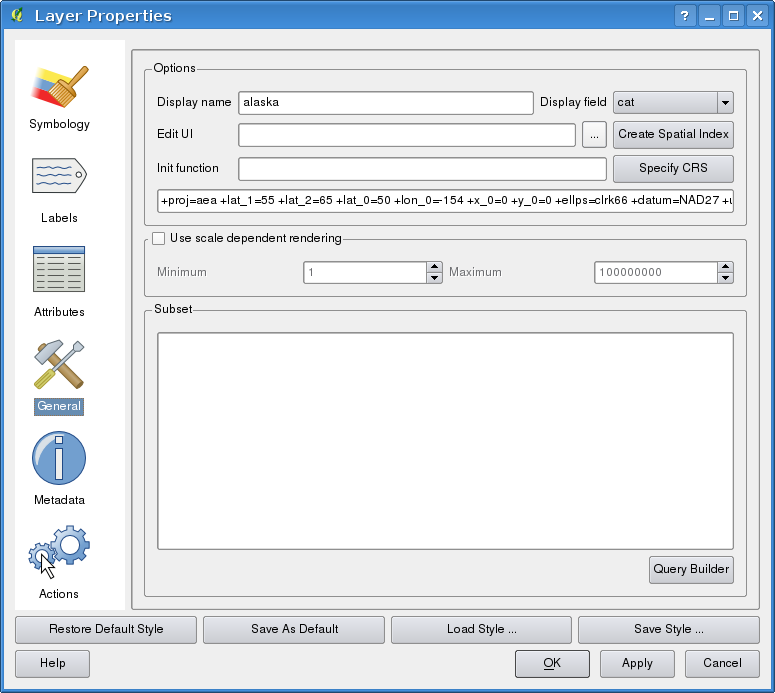
\includegraphics[clip=true, width=12cm]{vectorLayerSymbology} 
\end{center}  
\end{figure}

\subsubsection{General Tab}\label{vectorgeneraltab}
The \tab{General} tab is essentially like that of the raster dialog. It allows you
to change the display name, set scale dependent rendering options, create a spatial 
index of the vector file (only for OGR supported formats and PostGIS) and view or
change the projection of the specific vetor layer.

The \button{Query Builder} button allows you to create a subset of the features 
in the layer - but this button currently only is available when you open the 
attribute table and select the \button{Advanced ...} button.

\subsubsection{Symbology Tab}\label{sec:symbology}
\index{vector layers!symbology}

QGIS supports a number of symbology renderers to control how
vector features are displayed. Currently the following renderers
are available:

\begin{description} 
    \item[Single symbol] - a single style is applied to every
    object in the layer.\index{vector layers!renderers!single symbol}
    \item[Graduated symbol] - objects within the layer are
    displayed with different symbols classified by the values of a
    particular field.\index{vector layers!renderers!graduated symbol}
    \item[Continuous color] - objects within the layer are
    displayed with a spread of colours classified by the numerical
    values within a specified field.\index{vector layers!renderers!continuous
color}
    \item[Unique value] - objects are classified by the unique
    values within a specified field with each value having a
    different symbol.\index{vector layers!renderers!unique value}
\end{description}

To change the symbology for a layer, simply double click on its legend 
entry and the vector \dialog{Layer Properties} dialog will be 
shown.\index{symbology!changing}

\begin{figure}[h]
\centering
\caption{Symbolizing-options \nixcaption}
   \subfigure[Single symbol] {\label{subfig:single_symbol}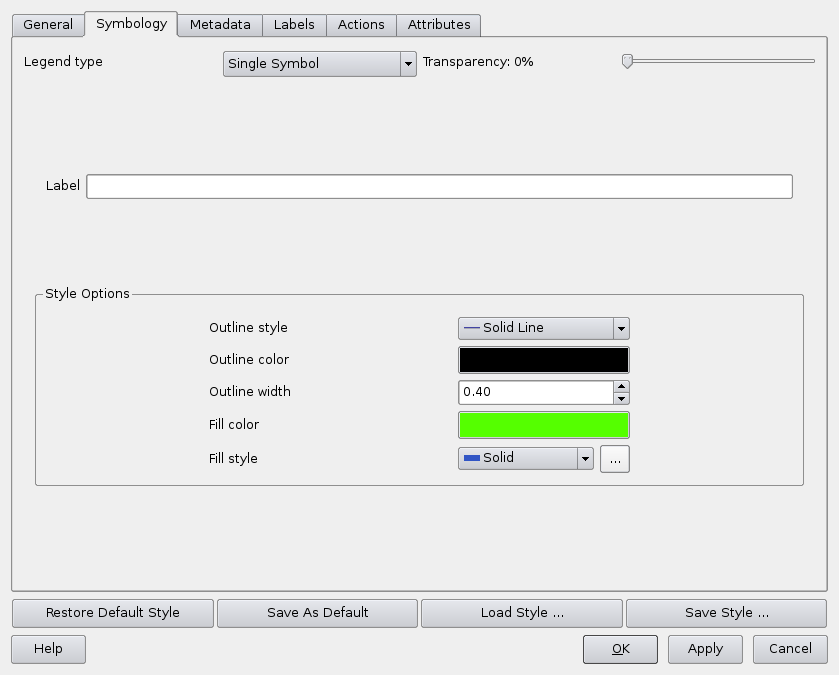
\includegraphics[clip=true, width=0.4\textwidth]{vectorClassifySingle}}\goodgap
   \subfigure[Graduated symbol] {\label{subfig:graduated_symbol}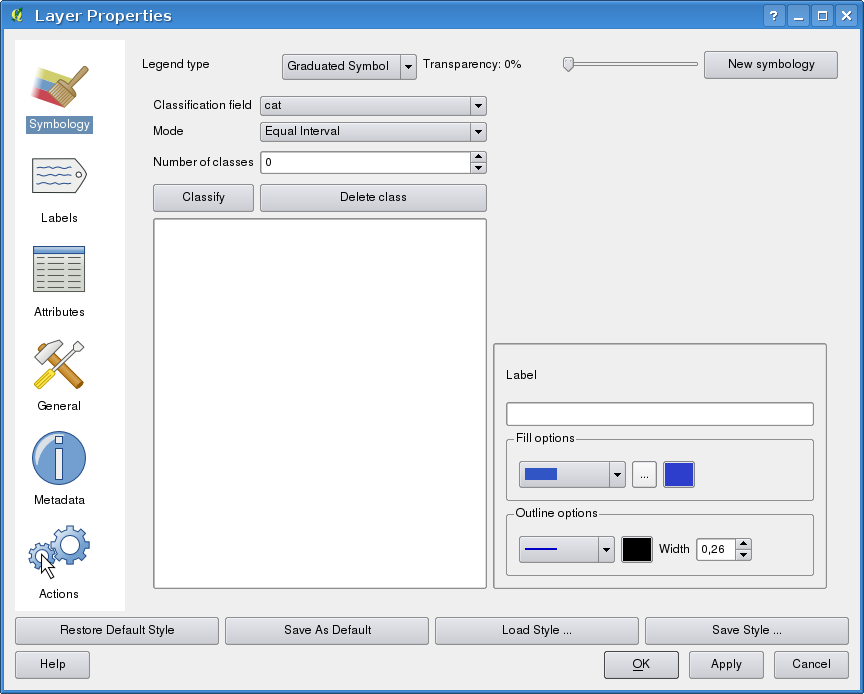
\includegraphics[clip=true, width=0.4\textwidth]{vectorClassifyGraduated}}\\
   \subfigure[Continous color] {\label{subfig:cont_color}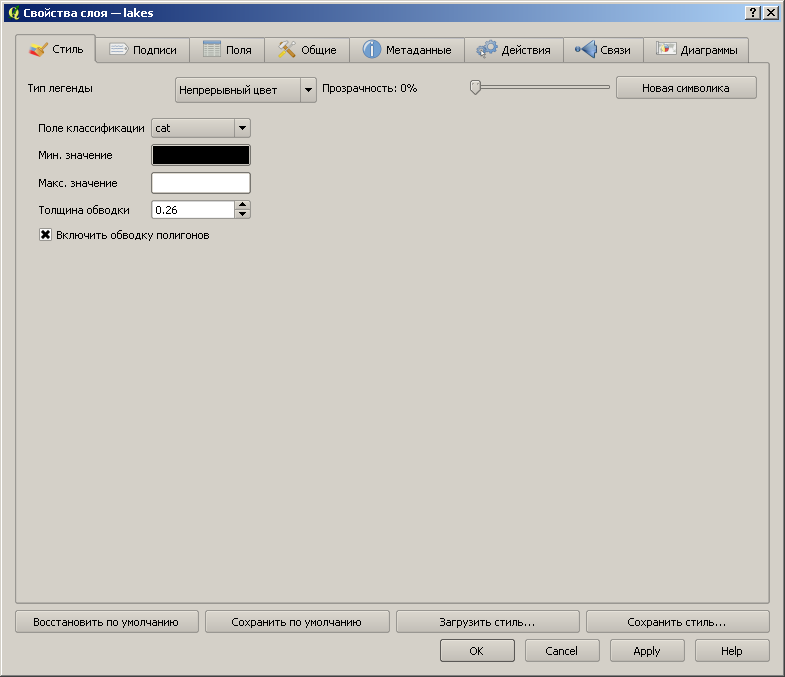
\includegraphics[clip=true, width=0.4\textwidth]{vectorClassifyContinous}}\goodgap
   \subfigure[Unique value] {\label{subfig:unique_val}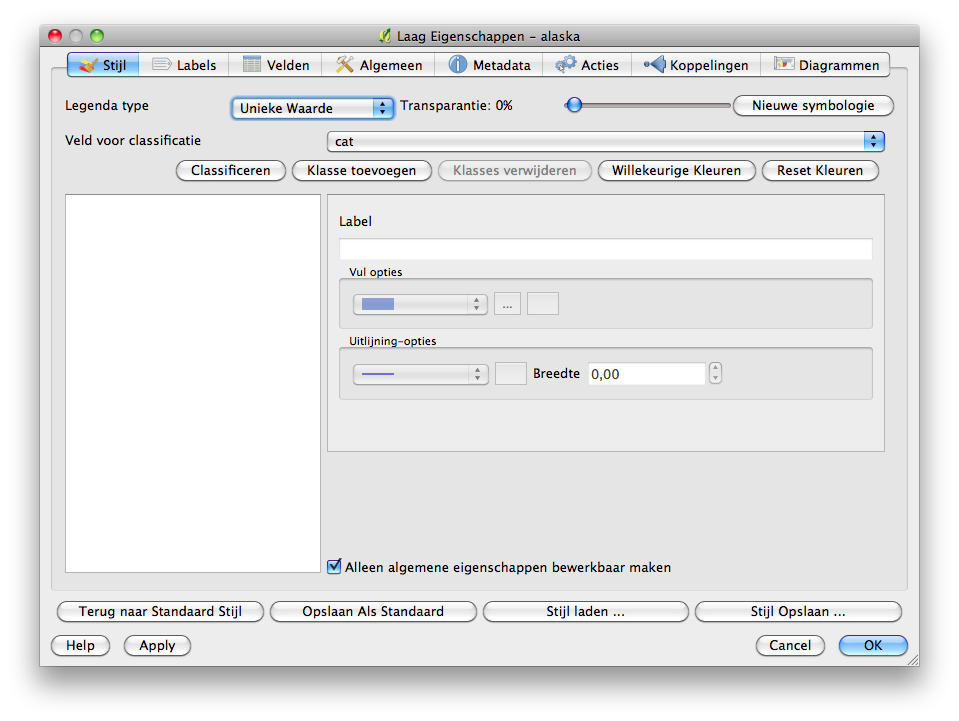
\includegraphics[clip=true, width=0.4\textwidth]{vectorClassifyUnique}}
\end{figure}

% FIXME: outdated
% Since \usertext{version v0.9} there is a function to use image files stored on 
% your computer as fill pattern for vector layers.

\minisec{Style Options} \label{sec:style_options} \index{vector layers!styles}
Within this dialog you can style your vector layer. Depending on the selected
rendering option you have the possibility to also classify your mapfeatures.

At least the following styling options apply for nearly all renderers:
\begin{description}
 \item[Outline style] - pen-style for your outline of your feature. you can
 also set this to 'no pen'.
 \item[Outline color] - color of the ouline of your feature
 \item[Outline width] - width of your features
 \item[Fill color] - fill-color of your features.
 \item[Fill style] - Style for filling. Beside the given brushes you can
 select \selectstring{Fill style}{? texture} and click the \browsebutton
 button for selecting your own fill-style. Currently the fileformats
 \filename{*.jpeg, *.xpm, and *.png} are supported.
\end{description}

Once you have styled your layer you also could save your layer-style to a
separate file (with \filename{*.qml}-ending).
To do this, use the button \button{Save Style \ldots}. No need to say that
\button{Load Style \ldots} loads your saved layer-style-file.

If you wish to always use a particular style whenever the layer is loaded, 
use the \button{Save As Default} button to make your style the default. Also, 
if you make changes to the style that you are not happy with, use the \button{Restore 
Default Styel} button to revert to your default style.

\minisec{Vector transparency} \label{sec:vect_transparency} \index{vector layers!transparency}
QGIS \CURRENT allows to set a transparency for every vector layer. This can be done with
the slider \slider{Transparency}{0}{20mm} inside the \tab{symbology} tab (see fig. \ref{fig:vector_symbology}).
This is very useful for overlaying several vector layers.

\subsubsection{Metadata Tab}

The \tab{Metadata} tab contains information about the layer, including specifics
about the type and location, number of features, feature type, and the editing
capabilities. The \guiheading{Layer Spatial Reference System} section, providing 
projection information, and the \guiheading{Attribute field info} section,
listing fields and their data types, are displayed 
on this tab. This is a quick way to get information about the layer.

\subsubsection{Labels Tab}

The \tab{Labels} tab allows you to enable labeling features and control a number of
options related to fonts, placement, style, alignment and buffering.

We will illustrate this by labelling the lakes shapefile of the
\filename{qgis\_example\_dataset}:

\begin{enumerate}
\item Load the Shapefile \filename{alaska.shp} and GML file \filename{lakes.gml} in QGIS.
\item Zoom in a bit to your favorite area with some lake.
\item Make the \filename{lakes} layer active.
\item Open the \dialog{Layer Properties} dialog.
\item Click on the \tab{Labels} tab.
\item Check the \checkbox{Display labels} checkbox to enable labeling.
\item Choose the field to label with. 
  We'll use \selectstring{Field containing label}{NAMES}.
\item Enter a default for lakes that have no name. The default label will be
  used each time QGIS encounters a lake with no value in the \guilabel{NAMES} field.
\item Click \button{Apply}.
\end{enumerate} 

Now we have labels. How do they look? They are probably too big and poorly
placed in relation to the marker symbol for the lakes.

Select the \tab{Font} entry and use the \button{Font} and \button{Color}
buttons to set the font and color. You can also change the angle and the
placement of the text-label.

To change the position of the text relative to the feature:

\begin{enumerate} 
\item Click on the \tab{Font} entry.
\item Change the placement by selecting one of the radio buttons
in the \classname{Placement} group. To fix our labels, choose the
\radiobuttonon{Right} radio button.
\item the \classname{Font size units} allows you to select between
\radiobuttonon{Points} or \radiobuttonon{Map units}.
\item Click \button{Apply} to see your changes without closing the dialog.
\end{enumerate} 

Things are looking better, but the labels are still too close to the marker. To
fix this we can use the options on the \tab{Position} entry. Here we can add
offsets for the X and Y directions. Adding an X offset of 5 will move our
labels off the marker and make them more readable. Of course if your marker
symbol or font is larger, more of an offset will be required.

The last adjustment we'll make is to \tab{buffer} the labels. This just means
putting a backdrop around them to make them stand out better. To buffer the
lakes labels:

\begin{enumerate}
\item Click the \tab{Buffer} tab.
\item Click the \checkbox{Buffer Labels?} checkbox to enable buffering.
\item Choose a size for the buffer using the spin box.
\item Choose a color by clicking on \button{Color} and choosing your
  favorite from the color selector. You can also set some transparency for the
  buffer if you prefer.
\item Click \button{Apply} to see if you like the changes.
\end{enumerate} 

If you aren't happy with the results, tweak the settings and then test again
by clicking \button{Apply}.

A buffer of 1 points seems to give a good result.
Notice you can also specify the buffer size in map units if that works out
better for you.

The remaining entries inside the \tab{Label} tab allow you control the appearance of the
labels using attributes stored in the layer. The entries beginning with \tab{Data defined} allow you to
set all the parameters for the labels using fields in the layer.

Not that the \tab{Label} tab provides a \classname{preview-box} where your
selected label is shown.

\subsubsection{Actions Tab}\index{actions}\label{label_actions}

QGIS provides the ability to perform an action based on the attributes of a
feature. This can be used to perform any number of actions, for example,
running a program with arguments built from the attributes of a feature or
passing parameters to a web reporting tool.

Actions are useful when you frequently want to run an external application or
view a web page based on one or more values in your vector layer. An example
is performing a search based on an attribute value. This concept is used in 
the following discussion.

\minisec{Defining Actions}\index{actions!defining}

Attribute actions are defined from the vector \dialog{Layer Properties} dialog. To
define an action, open the vector \dialog{Layer Properties} dialog and click on the
\tab{Actions} tab. Provide a descriptive name for the action. The action
itself must contain the name of the application that will be executed when the
action is invoked. You can add one or more attribute field values as arguments
to the application. When the action is invoked any set of characters that
start with a \% followed by the name of a field will be replaced by the value of
that field. The special characters \%\% \index{\%\%}will be replaced by the value
of the field that was selected from the identify results or attribute table (see
Using Actions below).  Double quote marks can be used to group text into a
single argument to the program, script or command. Double quotes will be
ignored if preceded by a backslash.

If you have field names that are substrings of other field names (e.g., \usertext{col1}
and \usertext{col10}) you should
indicate so, by surrounding the field name (and the \% character) with square
brackets (e.g., \usertext{[\%col10]}). This will prevent the \usertext{\%col10} field
name being mistaken for the \usertext{\%col1} field name with a \usertext{0}
on the end. The brackets will be removed by QGIS when it substitutes in the
value of the field. If you want the substituted field to be surrounded by square
brackets, use a second set like this: \usertext{[[\%col10]]}.

The \dialog{Identify Results} dialog box includes a {\em (Derived)} item that
contains information relevant to the layer type. The
values in this item can be accessed in a similar way to the other fields
by using preceeding the derived field name by \usertext{(Derived).}. For
example, a point layer has an \usertext{X} and \usertext{Y} field and the
value of these can be used in the action with \usertext{\%(Derived).X} and
\usertext{\%(Derived).Y}. The derived attributes are only available from the
\dialog{Identify Results} dialog box, not the \dialog{Attribute Table} dialog box.

Two example actions are shown below:\index{actions!examples}

\begin{itemize}
  \item \usertext{konqueror http://www.google.com/search?q=\%nam}
  \item \usertext{konqueror http://www.google.com/search?q=\%\%}
\end{itemize}

In the first example, the web browser konqueror is invoked and passed a URL to
open. The URL performs a Google search on the value of the \usertext{nam} field
from our vector layer. Note that the application or script called by the
action must be in the path or you must provided the full path. To be sure, we could
rewrite the first example as: \usertext{/opt/kde3/bin/konqueror
http://www.google.com/search?q=\%nam}. This will ensure that the konqueror
application will be executed when the action is invoked.

The second example uses the \%\% notation which does not rely on a particular
field for its value. When the action is invoked, the \%\% will be replaced by
the value of the selected field in the identify results or attribute table.

\minisec{Using Actions}\index{actions!using}\label{label_usingactions}
Actions can be invoked from either the \dialog{Identify Results} dialog or an
 \dialog{Attribute Table} dialog. 
(Recall that these dialogs can be opened by clicking
\toolbtntwo{mActionOpenTable}{Identify Features}
or
\toolbtntwo{mActionOpenTable}{Open Table}.)
To invoke an action, 
right click on the
record and choose the action from the popup menu. Actions are listed in the popup
menu by the name you assigned when defining the actions. Click on the action you
wish to invoke.

If you are invoking an action that uses the \%\% notation, right-click on the
field value in the \dialog{Identify Results} dialog or the
\dialog{Attribute Table} dialog that you wish to pass to the application or script.

Here is another example that pulls data out of a vector layer and inserts them
into a file using bash and the \usertext{echo} command (so it will only work
\nix or perhaps \osx). The layer in question has fields for a species name
\usertext{taxon\_name}, latitude \usertext{lat} and longitude
\usertext{long}. I would like to be able to
make a spatial selection of a localities and export these field values to a
text file for the selected record (shown in yellow in the QGIS map area). Here is
the action to achieve this:

\begin{verbatim}
  bash -c "echo \"%taxon_name %lat %long\" >> /tmp/species_localities.txt"
\end{verbatim} 

After selecting a few localities and running the action on each one, opening
the output file will show something like this:

\begin{verbatim}
  Acacia mearnsii -34.0800000000 150.0800000000
  Acacia mearnsii -34.9000000000 150.1200000000
  Acacia mearnsii -35.2200000000 149.9300000000
  Acacia mearnsii -32.2700000000 150.4100000000
\end{verbatim} 

As an exercise we create an action that does a Google search on the 
\filename{lakes} layer. First we need to determine the URL needed to perform a search on a
keyword. This is easily done by just going to Google and doing a simple
search, then grabbing the URL from the address bar in your browser. From this
little effort we see that the format is: \url{http://google.com/search?q=qgis},
where \usertext{qgis} is the search term. Armed with this information, we can
proceed:

\begin{enumerate}
\item Make sure the \filename{lakes} layer is loaded.
\item Open the \dialog{Layer Properties} dialog by double-clicking on the layer in the
  legend or right-click and choose \dropmenuopt{Properties} from the popup menu.
\item Click on the \tab{Actions} tab.
\item Enter a name for the action, for example \usertext{Google Search}.
\item For the action, we need to provide the name of the external program to
  run. In this case, we can use Firefox. If the program is not in
  your path, you need to provide the full path.
\item Following the name of the external application, add the URL used for
  doing a Google search, up to but not included the search term:
  \url{http://google.com/search?q=}
\item The text in the \guilabel{Action} field should now look like this:\\
  \usertext{firefox \url{http://google.com/search?q=}}
\item Click on the drop-down box containing the field names for the
  \usertext{lakes} layer. It's located just to the left of the
  \button{Insert Field} button.
\item From the drop-down box, select \selectstring{}{NAMES} and click \button{Insert Field}.
\item Your action text now looks like this:\\ \usertext{firefox
  \url{http://google.com/search?q=\%NAMES}}
\item Fo finalize the action click the \button{Insert action} button.
\end{enumerate}
 
This completes the action and it is ready to use. The final text of the action
should look like this:

\begin{center}
\usertext{firefox \url{http://google.com/search?q=\%NAMES}}
\end{center}

We can now use the action. Close the \dialog{Layer Properties} dialog and zoom in to an area
of interest. Make sure the \filename{lakes} layer is active and identify a
lake. In the result box you'll now see that our action is visible:

\begin{figure}[H]
   \begin{center}
   \caption{Select feature and choose action \nixcaption}\label{fig:identify_action}\smallskip
   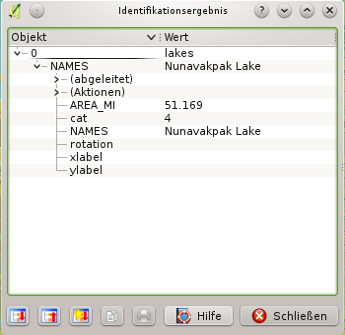
\includegraphics[clip=true, width=8cm]{action_identifyaction} 
\end{center}  
\end{figure}

When we click on the action, it brings up Firefox and navigates to the URL
\url{http://www.google.com/search?q=Tustumena}. It is also possible to add further 
attribute fields to the action. Therefore you can add a ``+'' to the end of the action 
text, select another field and click on \button{Insert Field}. In this example there 
is just no other field available that would make sense to search for.

You can define multiple actions for a layer and each will show up in the
\dialog{Identify Results} dialog. You can also invoke actions from the attribute table
by selecting a row and right-clicking, then choosing the action from the popup
menu.

You can think of all kinds of uses for actions. For example, if you have a point layer
containing locations of images or photos along with a file name, you could
create an action to launch a viewer to display the image. You could also use
actions to launch web-based reports for an attribute field or combination of
fields, specifying them in the same way we did in our Google search example.

\subsubsection{Attributes Tab}\index{attributes}\label{label_attributes}
Within the \tab{Attributes} tab the attributes of the selected dataset can be
manipulated. The buttons \button{New Column} and \button{Delete Column} can be
used, when the dataset is in editing mode. At the moment only columns from 
PostGIS layers can be edited, because this feature is not yet supported by 
the OGR library. 

The \button{Toggle editing mode} button toggles this mode.

\minisec{edit widget}

Within the \tab{Attributes} tab you also find an \texttt{edit widget} and a 
\texttt{value} column. These two columns can be used to define values or a range 
of values that are allowed to be added to the specific attribute table columns. 
They are used to produce different edit widgets in the attribute dialog. These 
widgets are:

\begin{itemize}
\item line edit: an edit field which allows to enter simple text (or restrict to 
numbers for numeric attributes).
\item unique value: a list of unique attribute values of all pre-existing features
is produced and presented in a combo box for selection.
\item  unique value (editable): a combination of `line edit' and `unique value'.
The edit field completes entered values to the unique value, but also allows
to enter new values.
\item value map: a combobox to select from a set of values specified in the
\texttt{value} column the \tab{Attributes} tab.  The possible values are 
delimited by a semicolon (e.g. \verb|high;medium;low|).  It is also possible
to prepend a label to each value, which is delimited with an equal sign (e.g.
\verb|high=1;medium=2;low=3|). The label is shown in the combobox instead of
the value.
\item classification: if a unique value renderer is selected for the layer, the
values used for the classes are presented for selection in a combobox.
\item range (editable): A edit field that allows to restrict numeric values to a
given range.  That range is specified by entering minium and maximum value
delimited by a semicolon (e.g. \verb|0;360|) in the \texttt{value} column of
the \tab{Attributes} tab.
\item range (slider): A slider widget is presented that allows selection of a value
in a given range and precision.  The range is specifed by minimum, maximum
value and a step width (e.g. \verb|0;360;10|) in the \texttt{value} column of
the \tab{Attributes} tab.
\item file name: the line edit widget is accompanied by a push button. When pressed
it allows to select a filename using the standard file dialog.
\end{itemize}

\subsection{Editing}\index{editing}

QGIS supports basic capabilities for editing vector geometries.  Before reading any
further you should note that at this stage editing support is still preliminary.
Before performing any edits, always make a backup of the dataset you are about
to edit. 

\textbf{Note} - the procedure for editing GRASS layers is different - see
Section \ref{grass_digitising} for details.

\subsubsection{Setting the Snapping Tolerance and Search Radius}

Before we can edit vertices, it is very important to set the snapping
tolerance and search radius to a value that allows us an optimal editing of
the vector layer geometries. 

\minisec{Snapping tolerance}

Snapping tolerance is the distance QGIS uses to \usertext{search} for the
closest vertex and/or segment you are trying to
connect when you set a new vertex or move an existing vertex. If you aren't
within the snap tolerance, QGIS will leave the vertex where you release the
mouse button, instead of snapping it to an existing vertex and/or segment. 

\begin{enumerate}
\item A general, project wide snapping tolerance can be defined choosing
\mainmenuopt{Settings} > \dropmenuopttwo{mActionOptions}{Options}
In the \tab{Digitizing} tab you can select between to vertex, to segment or
to vertex and segment as default snap mode. You can also define a default
snapping tolerance and a search radius for vertex edits. Remember the
tolerance is in layer units. In our digitizing project (working with the
Alaska dataset), the units are in feet. Your results may vary, but something
on the order of 300ft should be fine at a scale of 1:10 000 should be a
reasonable setting.
\item A layer based snapping tolerance can be defined by choosing
\mainmenuopt{Settings} > \dropmenuopttwo{mActionOptions}{Project
Properties\dots}. In the \tab{General} tab, section \classname{Digitize} you
can click on \button{Snapping options\dots} to enable and adjust snapping
mode and tolerance on a layer basis (see Figure~\ref{fig:snappingoptions}).
\end{enumerate}

\begin{figure}[H]
   \begin{center}
   \caption{Edit snapping options on a layer basis \nixcaption}\label{fig:snappingoptions}\smallskip
   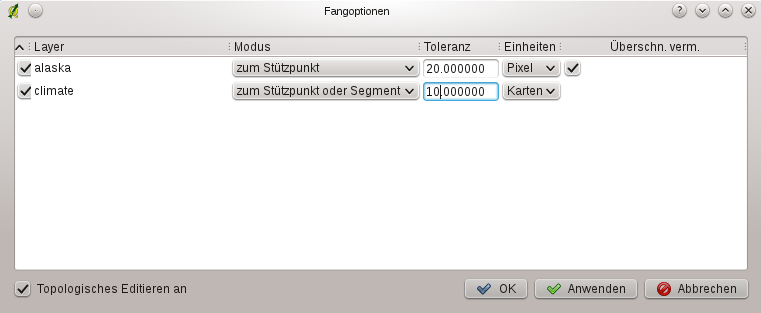
\includegraphics[clip=true, width=14cm]{editProjectSnapping} 
\end{center}  
\end{figure}

\minisec{Search radius}

Search radius is the distance QGIS uses to \usertext{search} for the closest
vertex you are trying to move when you click on the
map. If you aren't within the search radius, QGIS won't find and select
any vertex for editing and it will pop up an annoying warning to that effect.
Snap tolerance and search radius are set in map units so you may find you
need to experiment to get them set right. If you specify too big of a
tolerance, QGIS may snap to the wrong vertex, especially if you are dealing
with a large number of vertices in close proximity. Set search radius too
small and it won't find anything to move.

The search radius for vertex edits in layer units can be defined in the
\tab{Digitizing} tab under \mainmenuopt{Settings} >
\dropmenuopttwo{mActionOptions}{Options}. The same place where you define the
general, project wide snapping tolerance.

\subsubsection{Topological editing}

Besides layer based snapping options the \tab{General} tab in menu 
\mainmenuopt{Settings} -> \dropmenuopttwo{mActionOptions}{Project Properties\dots} 
also provides some topological functionalities. 
In the Digitizing option group you can \checkbox{Enable topological editing} and/or activate 
\checkbox{Avoid intersections of new polygons}.

\minisec{Enable topological editing}

The option \checkbox{Enable topological editing} is for editing and maintaining 
common boundaries in polygon mosaics. QGIS "detects" a shared boundary in 
a polygon mosaic and you only have to move the vertex once and QGIS will take 
care about updating the other boundary.

\minisec{Avoid intersections of new polygons}

The second topological option called \checkbox{Avoid intersections of new polygons} 
avoids overlaps in polygon mosaics. It is for quicker digitizing of adjacent polygons. 
If you already have one polygon, it is possible with this option to digitise the second 
one such that both intersect and qgis then cuts the second polygon to the common boundary. 
The advantage is that users don't have to digitize all vertices of the common boundary.

\subsubsection{Editing an Existing Layer}
\index{vector layers!editing}
\index{editing!an existing layer}
\label{sec:edit_existing_layer}

By default, QGIS loads layers read-only: This is a safeguard
to avoid accidentally editing a layer if there is a slip of the mouse.
However, you can choose to edit any layer as long as the data provider supports it,
and the underlying data source is writable (i.e. its files are not read-only).

Layer editing is most versatile when used on PostgreSQL/PostGIS data sources. 

\begin{Tip}[ht]\caption{\textsc{Data Integrity}}
\qgistip{It is always a good idea to back up your data source before you start 
editing. While the authors of QGIS have made every effort to preserve the 
integrity of your data, we offer no warranty in this regard.
}
\end{Tip}

\begin{Tip}[ht]\caption{\textsc{Manipulating Attribute data}}
\qgistip{Currently only PostGIS layers are supported for adding or dropping attribute
columns within this dialog. In future versions of QGIS, other datasources 
will be supported, because this feature was recently implemented in GDAL/OGR > 1.6.0
}
\end{Tip}



\begin{Tip}[ht]\caption{\textsc{Save Regularly}}
\qgistip{Remember to toggle \toolbtntwo{mActionToggleEditing}{Toggle editing} off regularly.  
This allows you to save your recent changes,
and also confirms that your data source can accept all
your changes.
}
\end{Tip}

\begin{Tip}[ht]\caption{\textsc{Concurrent Edits}}
\qgistip{This version of QGIS does not track if somebody else is editing a feature at the same time
as you.  The last person to save their edits wins.
}
\end{Tip}

\begin{Tip}[ht]\caption{\textsc{Zoom in Before Editing}}
\qgistip{Before editing a layer, you should
zoom in to your area of interest. This 
avoids waiting while all the vertex markers are rendered across the entire layer.
}
\end{Tip}

\begin{Tip}[ht]\caption{\textsc{Vertex Markers}}
\qgistip{
The current version of QGIS supports several two kinds of vertex-markers -
a semi-transparent circle or a cross. To change the marker style, choose
\dropmenuopttwo{mActionOptions}{Options} from the
\mainmenuopt{Settings} menu and click on the \tab{Digitizing} tab and select
the appropriate entry.
}
\end{Tip}

All editing sessions start by choosing the \dropmenuopttwo{mActionToggleEditing}{Toggle editing} option.
This can be found in the context menu after right clicking on the legend
entry for that layer.\index{Allow Editing}
Alternately, you can use the \index{Toggle Editing}
\toolbtntwo{mActionToggleEditing}{Toggle editing} button from the toolbar to start 
or stop the editing mode.\index{editing!icons} Once the layer is in edit mode, 
markers will appear at the vertices, and additional tool buttons on the editing 
toolbar will become available.

\minisec{Zooming with the mouse wheel}

While digitizing you can use the mouse wheel to zoom in and out on the map 
Place the mouse cursor inside the map area and roll it forward (away from you) 
to zoom in and backwards (towards you) to zoom out. The mouse cursor position will 
be the center of the zoomed area of interest. You can customize the behavior 
of the mouse wheel zoom using the \tab{Map tools} tab under the \mainmenuopt{Settings} 
>\dropmenuopt{Options} menu.

\minisec{Panning with the arrow keys}

Panning the Map during digitizing is possible with the arrow keys. Place
the mouse cursor inside the map area and click on the right arrow key to
pan east, left arrow key to pan west, up arrow key to pan north and down arrow 
key to pan south.

You can also use the spacebar to temporarily cause mouse movements to pan 
then map. The PgUp and PgDown keys on your keyboard will cause the map 
display to zoom in or our without interupting your digitising session.

You can perform the following editing functions:

\begin{itemize}
\item Add Features: \toolbtntwo{mActionCapturePoint}{Capture Point},
  \toolbtntwo{mActionCaptureLine}{Capture Line} and
  \toolbtntwo{mActionCapturePolygon}{Capture Polygon}
\item \toolbtntwo{mActionAddRing}{Add Ring}
\item \toolbtntwo{mActionAddIsland}{Add Island}
\item \toolbtntwo{mActionSplitFeatures}{Split Features}
\item \toolbtntwo{mActionMoveFeature}{Move Features}
\item \toolbtntwo{mActionMoveVertex}{Move Vertex}
\item \toolbtntwo{mActionAddVertex}{Add Vertex}
\item \toolbtntwo{mActionDeleteVertex}{Delete Vertex}
\item \toolbtntwo{mActionDeleteSelected}{Delete Selected}
\item \toolbtntwo{mActionEditCut}{Cut Features}
\item \toolbtntwo{mActionEditCopy}{Copy Features}
\item \toolbtntwo{mActionEditPaste}{Paste Features}
\end{itemize}

\minisec{Adding Features}
\index{vector layers!adding!feature}

Before you start adding features, use the \toolbtntwo{mActionPan}{pan}
and \toolbtntwo{mActionZoomIn}{zoom-in}/\toolbtntwo{mActionZoomOut}{zoom-out} 
tools to first navigate to the area of interest.

Then you can use the \toolbtntwo{mActionCapturePoint}{Capture point},
\toolbtntwo{mActionCaptureLine}{Capture line} or
\toolbtntwo{mActionCapturePolygon}{Capture polygon} icons on the toolbar to put the QGIS cursor
into digitizing mode.

For each feature, you first digitize the geometry, then enter its attributes.

To digitize the geometry, left-click on the map area to create the
first point of your new feature.

For lines and polygons, keep on left-clicking for each additional
point you wish to capture.  When you have finished adding points,
right-click anywhere on the map area to confirm you have finished entering
the geometry of that feature.

The attribute window will appear, allowing you to enter the information for the new feature.
Figure \ref{fig:vector_digitising} shows setting attributes for a fictitious
new river in Alaska.

\begin{figure}[ht]
   \begin{center}
   \caption{Enter Attribute Values Dialog after digitizing a new vector
   feature \nixcaption}\label{fig:vector_digitising}\smallskip
   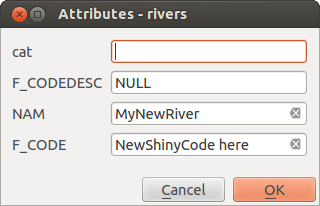
\includegraphics[clip=true, width=8cm]{editDigitizing}
\end{center}  
\end{figure}

\begin{Tip}[ht]\caption{\textsc{Attribute Value Types}}
\qgistip{
At least for shapefile editing the attribue types are validated during the
entry. Because of this, it is not possible to enter a number into the text-column in
the dialog \dialog{Enter Attribute Values} or vica versa. If you need to do so,
you should edit the attributes in a second step within the \dialog{Attribute
table} dialog.
}
\end{Tip}

\minisec{Move Feature}
\index{vector layers!move!feature}

You can move features using the \toolbtntwo{mActionMoveFeature}{Move Feature} icon
on the toolbar.

\minisec{Split Feature}
\index{vector layers!split!feature}

You can split features using the \toolbtntwo{mActionSplitFeatures}{Split Features} icon
on the toolbar.

\minisec{Editing Vertices of a Feature}
\index{vector layers!editing!vertex}

For both PostgreSQL/PostGIS and shapefile-based layers, the vertices of features can be edited. 

Vertices can be directly edited, that is, you don't
have to choose which feature to edit before you can change
its geometry.
In some cases, several features may share the same vertex
and so the following rules apply when the mouse is pressed
down near map features:

\begin{itemize}
\item \textbf{Lines}    - The nearest line to the mouse position
                          is used as the target feature.
                          Then (for moving and deleting a vertex)
                          the nearest vertex
                          on that line is the editing target.

\item \textbf{Polygons} - If the mouse is inside a polygon, then it is
                          the target feature; otherwise the nearest polygon
                          is used.
                          Then (for moving and deleting a vertex)
                          the nearest vertex
                          on that polygon is the editing target.
\end{itemize}

You will need to set the property
\mainmenuopt{Settings}>\dropmenuopttwo{mActionOptions}{Options}>\tab{Digitizing}
to a number greater than zero.  Otherwise QGIS will not be able to tell which feature is being edited.


\minisec{Adding Vertices of a Feature}
\index{vector layers!adding!vertex}

You can add new vertices to a feature by using the
\toolbtntwo{mActionAddVertex}{Add Vertex} icon
on the toolbar.

Note, it doesn't make sense to add more vertices to a Point feature!

In this version of QGIS, vertices can only be added to an \textit{existing} line
segment of a line feature.  If you want to extend a line beyond its end,
you will need to move the terminating vertex first, then add a new vertex where
the terminus used to be.

\minisec{Moving Vertices of a Feature}
\index{vector layers!moving!vertex}

You can move vertices using the \toolbtntwo{mActionMoveVertex}{Move Vertex} icon
on the toolbar.

\minisec{Deleting Vertices of a Feature}
\index{vector layers!deleting!vertex}

You can delete vertices by using the \toolbtntwo{mActionDeleteVertex}{Delete Vertex} icon
on the toolbar.

Note, it doesn't make sense to delete the vertex of a Point feature!
Delete the whole feature instead.

Similarly, a one-vertex line or a two-vertex polygon is also
fairly useless and will lead to unpredictable results elsewhere
in QGIS, so don't do that.

\textbf{Warning:} A vertex is identified for deletion as
soon as you click the mouse near an eligible
feature.  To undo, you will need to toggle
Editing off and then discard your changes.
(Of course this will mean that other unsaved changes will be lost, too.)

\minisec{Add Ring}
\index{vector layers!add!ring}

You can create ring polygons using the \toolbtntwo{mActionAddRing}{Add Ring}
icon in the toolbar. This means inside an existing area it is
possible to digitize further polygons, that will occur as a 'whole', so only 
the area in between the boundaries of the outer and inner polygons remain as 
a ring polygon. 

\minisec{Add Island}
\index{vector layers!add!island}

You can \toolbtntwo{mActionAddIsland}{add island} polygons to a selected multipolygon. 
The new island polygon has to be digitized outside the selected multipolygon. 

\minisec{Cutting, Copying and Pasting Features}
\index{vector layers!cut!feature}
\index{vector layers!copy!feature}
\index{vector layers!paste!feature}
\index{editing!cutting features}
\index{editing!copying features}
\index{editing!pasting features}

Selected features can be cut, copied and pasted between layers in the
same QGIS project, as long as destination layers are set to 
\toolbtntwo{mActionToggleEditing}{Toggle editing} beforehand.

Features can also be pasted to external applications as text:  That is,
the features are represented in CSV format with the geometry data appearing 
in the OGC Well-Known Text (WKT) format.


However in this version of QGIS, text features from outside QGIS cannot 
be pasted to a layer within QGIS. When would the copy and paste function 
come in handy? Well, it turns out that you can edit more than one layer 
at a time and copy/paste features between layers. Why would we want to do 
this?  Say we need to do some work on a new layer but only need one or 
two lakes, not the 5,000 on our \filename{big\_lakes} layer. We can create 
a new layer and use copy/paste to plop the needed lakes into it. 

As an example we are copying some lakes to a new layer:

\begin{enumerate}
\item Load the layer you want to copy from (source layer)
\item Load or create the layer you want to copy to (target layer) 
\item Start editing for both layers 
\item Make the source layer active by clicking on it in the legend 
\item Use the \toolbtntwo{mActionSelect}{Select} tool to select the feature(s) on the source layer
\item Click on the \toolbtntwo{mActionEditCopy}{Copy Features} tool
\item Make the destination layer active by clicking on it in the legend 
\item Click on the \toolbtntwo{mActionEditPaste}{Paste Features} tool 
\item Stop editing and save the changes
\end{enumerate}

What happens if the source and target layers have
different schemas (field names and types are not the same)? QGIS populates
what matches and ignores the rest. If you don't care about the attributes
being copied to the target layer, it doesn't matter how you design the
fields and data types. If you want to make sure everything - feature and its
attributes - gets copied, make sure the schemas match.

\begin{Tip}[ht]\caption{\textsc{Congruency of Pasted Features}}
\qgistip{If your source and destination layers use the
same projection, then the pasted features will have
geometry identical to the source layer.
However if the destination layer is a different projection
then QGIS cannot guarantee the geometry is identical.
This is simply because there are small rounding-off errors
involved when converting between projections.
}
\end{Tip}

\minisec{Deleting Selected Features}
\index{vector layers!deleting!feature}

If we want to delete an entire polygon, we can do that by first selecting 
the polygon using the regular \toolbtntwo{mActionSelect}{Select Features} tool. You can select 
multiple features for deletion. Once you have the selection set, use the 
\toolbtntwo{mActionDeleteSelected}{Delete Selected} tool to delete the features. There is no undo function, 
but remember your layer isn't really changed until you stop editing and choose 
to save your changes. So if you make a mistake, you can always cancel the save.

The \toolbtntwo{mActionEditCut}{Cut Features} tool on the digitizing toolbar can
also be used to delete features. This effectively deletes the feature but
also places it on a ``spatial clipboard". So we cut the feature to delete. 
We could then use the \toolbtntwo{mActionEditPaste}{paste tool} to put it back, giving us a one-level undo 
capability. Cut, copy, and paste work on the currently selected features, 
meaning we can operate on more than one at a time.

\begin{Tip}[ht]\caption{\textsc{Feature Deletion Support}}
\qgistip{When editing ESRI shapefiles, the deletion
of features only works if QGIS is linked to a GDAL version 1.3.2 or greater. 
The OS X and Windows versions of QGIS available from the download site are built 
using GDAL 1.3.2 or higher.
}
\end{Tip}

\minisec{Snap Mode}
\index{editing!snap}
QGIS allows digitized vertices to be snapped to other vertices of the same layer. To 
set the snapping tolerance, go to
\mainmenuopt{Settings}>\dropmenuopttwo{mActionOptions}{Options}->\tab{Digitizing}.
Note that the snapping tolerance is in map units.

\minisec{Saving Edited Layers}
\index{editing!saving changes}

When a layer is in editing mode, any changes remain in the memory of QGIS.
Therefore they are not committed/saved immediately to the data source or disk.
When you turn editing mode off (or quit QGIS for that matter), 
you are then asked if you want to save your
changes or discard them.

If the changes cannot be saved (e.g. disk full, or the attributes have
values that are out of range), the QGIS in-memory state is preserved.  This
allows you to adjust your edits and try again.

\subsubsection{Creating a New Layer}\label{sec:create shape}\index{editing!creating a new layer}

To create a new layer for editing, choose \toolbtntwo{mActionNewVectorLayer}{New Vector Layer} from the
\mainmenuopt{Layer} menu. 
The \dialog{New Vector Layer} dialog will be displayed as
shown in Figure \ref{fig:newvectorlayer}. Choose the type of layer (point,
line or polygon).

\begin{figure}[ht]
   \begin{center}
   \caption{Creating a New Vector Dialog \nixcaption}\label{fig:newvectorlayer}\smallskip
   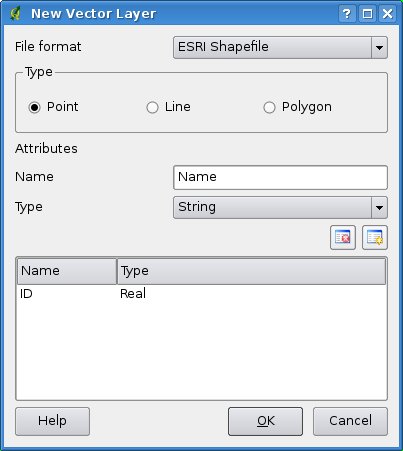
\includegraphics[clip=true, width=10cm]{editNewVector}
\end{center} 
\end{figure}

Note that QGIS does not yet support creation of 2.5D
features (i.e. features with X,Y,Z coordinates) or measure features. At this
time, only shapefiles can be created. In a future version of QGIS, creation of
any OGR or PostgreSQL layer type will be supported. 

Creation of GRASS-layers is supported within the GRASS-plugin. Please refer to section
\ref{sec:creating_new_grass_vectors} for more information on creating GRASS vector 
layers.

To complete the creation of the new layer, add the desired attributes by
clicking on the \button{Add} button and specifying a name and type for the
attribute. Only \selectstring{Type}{real}, \selectstring{Type}{integer}, and \selectstring{Type}{string} attributes are supported. Once you
are happy with the attributes, click \button{OK} and provide a name for the shapefile.
QGIS will automatically add a \filename{.shp} extension to the name you specify.  Once
the layer has been created, it will be added to the map and you can edit it in
the same way as described in Section \ref{sec:edit_existing_layer} above. 

\subsection{Query Builder}\label{sec:query_builder}
\index{Query Builder}

The Query Builder allows you to define a subset of a table and display
it as a layer in QGIS. It can currently only be used with PostGIS layers. 
For example, if you have a \filename{towns} layer with a
\usertext{population} field you could select only larger towns by entering
\usertext{population > 100000} in the SQL box of the query builder. Figure
\ref{fig:query_builder} shows an example of the query builder populated with
data from a PostGIS layer with attributes stored in PostgreSQL. 

\begin{figure}[ht]
  \begin{center}
    \caption{Query Builder \nixcaption}\label{fig:query_builder}\smallskip
    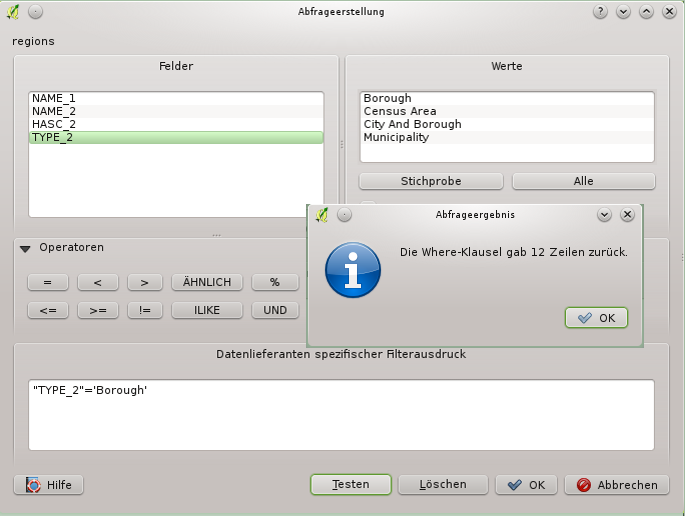
\includegraphics[clip=true, width=11.5cm]{queryBuilder}
  \end{center}  
\end{figure}

The query builder\index{Query Builder} lists the layer's database
fields in the list box on the left. You can get a sample of the data
contained in the highlighted field by clicking on the \button{Sample} button\index{Query
Builder!generating sample list}. This retrieves the first 25 distinct values
for the field from the database. To get a list of all possible values for a
field, click on the \button{All} button\index{Query Builder!getting all
values}. To add a selected field or value to the query, double-click on
it\index{Query Builder!adding fields}. You can use the various buttons to
construct the query or you can just type it into the SQL box.

To test a query, click on the \button{Test} button\index{Query Builder!testing
queries}. This will return a count of the number of records that will be
included in the layer. When satisfied with the query, click \button{OK}. The
SQL for the where clause will be shown in the SQL column of the layer list.

\begin{Tip}\caption{\textsc{Changing the Layer Definition}}\index{Query
Builder!changing layer definitions}
\qgistip{You can change the layer definition after it is loaded by altering
the SQL query used to define the layer. To do this, open the 
vector \dialog{Layer Properties} dialog by double-clicking on the layer in the legend and click on the
\button{Query Builder} button on the \tab{General} tab. See Section
\ref{sec:vectorprops} for more information.}
\end{Tip}

\subsection{Select by query}\label{sec:select_by_query}
\index{PostgreSQL!query builder}
\index{PostGIS!query builder}
\index{query builder!PostgreSQL}
\index{query builder!PostGIS}

With QGIS it is possible also to select features using a similar query builder 
interface to that used in \ref{sec:query_builder}. In the above section 
the purpose of the query builder is to only show features meeting the 
filter criteria as a 'virtual layer' / subset. The purpose of the select by 
query function is to highlight all features that meet a particular criteria. 
Select by query can be used with all vector data providers.

To do a `select by query' on a loaded layer, click on the 
button \toolbtntwo{mActionOpenTable}{Open Table} to open the attribute table of the layer. Then 
click the \button{Advanced...} button at the bottom. This starts the Query Builder 
that allows to define a subset of a table and display it as described in Section 
\ref{sec:query_builder}.


\index{vector layers|)}

\section{Working with Raster Data}\label{label_raster}
\index{raster layers|(}

QGIS supports a number of raster data formats. This section describes how to
work with raster data in QGIS.

\subsection{What is raster data?}\label{label_whatsraster}
\index{raster layers!definition}

Raster data in GIS are matrices of discrete cells that represent features on,
above or below the earth's surface. Each cell in the raster grid is the same
size, and cells are usually rectangular (in QGIS they will always be
rectangular). Typical raster datasets include remote sensing data such as
aerial photography or satellite imagery and modelled data such as an elevation
matrix.

Unlike vector data, raster data typically do not have an associated database
record for each cell.

In GIS, a raster layer would have georeferencing data associated with it which
will allow it to be positioned correctly in the map display to allow other
vector and raster data to be overlaid with it. QGIS makes use of georeferenced
rasters to properly display the data.\index{raster layers!georeferenced}
	
\subsection{Raster formats supported in QGIS}\label{label_rastformats}
QGIS supports a number of different raster formats. Currently tested formats
include:\index{raster layers!data formats}

\begin{itemize}
\item Arc/Info Binary Grid
\item Arc/Info ASCII Grid
\item GRASS Raster
\item GeoTIFF
\item JPEG
\item Spatial Data Transfer Standard Grids (with some limitations)
\item USGS ASCII DEM
\item Erdas Imagine
\end{itemize}

Because the raster implementation in QGIS is based on the GDAL library, other
raster formats implemented in GDAL are also likely to work, but have not yet
been tested. See Appendix \ref{appdx_gdal} for more
details.\index{raster layers!GDAL implementation}
	
\subsection{Loading raster data in QGIS}\label{label_loadraster}

Raster layers are loaded either by clicking on the 
\toolbtntwo{mActionAddRasterLayer}{Load Raster} icon or by
selecting the \mainmenuopt{View}>\dropmenuopttwo{mActionAddRasterLayer}{Add Raster Layer} menu option. More than one 
layer can be loaded at the same time by holding down the
\keystroke{Control} or \keystroke{Shift} key
and clicking on multiple items in the dialog \dialog{Open a GDAL Supported
Raster Data Source}.\index{raster layers!loading}

Please refer to section \ref{sec:load_grassdata} if you intend to load GRASS rasterdata.
	
\subsection{Raster Properties Dialog}\label{label_rasterprop}

To view and set the \dropmenuopt{properties} for a raster layer, right click on the layer
name. This displays the raster layer context menu that includes a number of
items that allow you to:\index{raster layers!context menu}
% FIXME
%\begin{figure}[ht]
%   \begin{center}
%   \caption{Raster context menu}\label{fig:raster_contextmenu}\smallskip
%   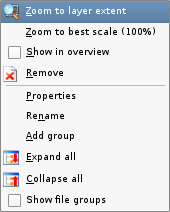
\includegraphics[clip=true, width=5cm]{rastercontextmenu}
%\end{center}  
%\end{figure}

\begin{itemize}
\item \toolbtntwo{mActionZoomFullExtent}{Zoom to the full extent} of the raster
\item Zoom to the best scale of the raster
\item Show the raster in the map overview window
\item \toolbtntwo{mActionRemoveLayer}{Remove layer} from the map
\item Open the raster layers properties
\item Rename the layer
\item Add a layer group
\item \toolbtntwo{mActionExpandTree}{Expand legend tree view}
\item \toolbtntwo{mActionCollapseTree}{Collapse legend tree view}
\item Show file groups
\end{itemize}

Choose \dropmenuopt{Properties} from the context menu to open the
\button{Raster Layer Properties}
dialog for the layer.\index{raster layers!properties}

Figure \ref{fig:raster_properties} shows the \dialog{Raster Layer
Properties} dialog. There are five
tabs on the dialog: \tab{Symbology}, \tab{General}, \tab{Metadata}, \tab{Pyramids} and \tab{Histogram}.

% FIXME
%\begin{figure}[h]
%   \begin{center}
%   \caption{Raster Layers Properties
%Dialog}\label{fig:raster_properties}\smallskip
%   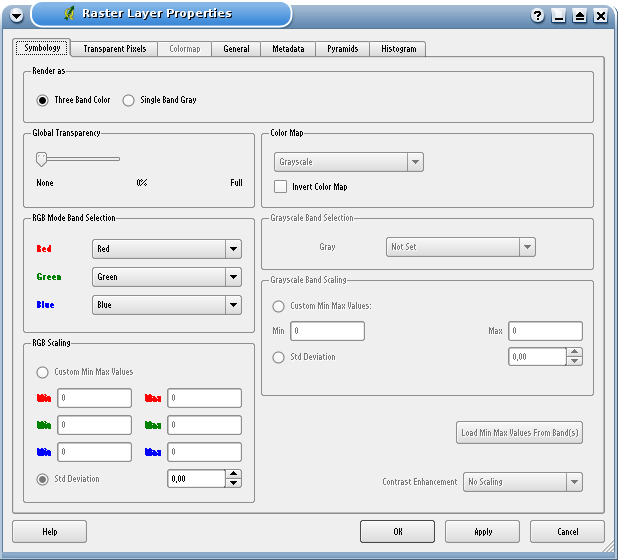
\includegraphics[clip=true, width=14cm]{raster_properties}
%\end{center}  
%\end{figure}

\subsubsection{Symbology Tab}\label{label_sombology}

QGIS supports three forms of raster layers:\index{raster layers!supported channels}

\begin{itemize}
\item Single Band Grayscale Rasters
\item Palette Based RGB Rasters
\item Multiband RGB Rasters
\end{itemize}

From these three basic layer types, eight forms of symbolised raster display
can be used:\index{raster layers!rendering interpretation}

\begin{itemize}
\item Single Band Grayscale
\item Single Band Pseudocolor
\item Paletted Grayscale (where only the red, green or blue component of the
image is displayed)
\item Paletted Pseudocolor (where only the red, green or blue component of the
image is displayed, but using a pseudocolor algorithm)
\item Paletted RGB
\item Multiband Grayscale (using only one of the bands to display the image)
\item Multiband Pseudocolor (using only one of the bands shown in
pseudocolor)
\item Multiband RGB (using any combination of three bands)
\end{itemize}

\smallskip

QGIS can invert the colors in a given layer so that light colors become dark
(and dark colors become light). Use the \checkbox{Invert Color Map} checkbox to
enable / disable this behavior.\index{raster layers!icolor map inversion}

QGIS has the ability to display each raster layer at varying transparency
levels.\index{raster layers!transparency} Use the transparency slider to indicate to
what extent the underlying layers (if any) should be visible though the
current raster layer. 

QGIS can restrict the data displayed to only show cells whose values are
within a given number of standard deviations of the mean for the
layer.\index{raster layers!standard deviation} This is useful when you have one or
two cells with abnormally high values in a raster grid that are having a
negative impact on the rendering of the raster. This option is only available
for pseudocolor images.

\begin{Tip}\caption{\textsc{Viewing a Single Band of a Multiband Raster}}
\qgistip{If you want to view a single band (for example Red) of a multiband
image, you might think you would set the Green and Blue bands to ``Not
Set''. But this is not the correct way. To display the Red band, 
set the image type to grayscale, then select Red as the band to use for Gray.
}
\end{Tip} 

\subsubsection{General Tab}\label{label_generaltab}

The \tab{General} tab displays basic information about the selected raster,
including the layer source and  display name in the legend (which can be
modified). This tab also shows a thumbnail of the layer, its legend symbol,
and the palette.\index{raster layers!properties}

Additionally scale-dependent visability can be set in this tab. You need to
check the checkbox and set an appropriate scale where your data will be
displayed in the map canvas.

Also the spatial reference system is printed here as a PROJ.4-string. 
This can be modified by hitting the \button{Change} button.

\subsubsection{Metadata Tab}\label{label_metatab}

The \tab{Metadata} tab displays a wealth of information about the raster layer,
including statistics about each band in the current raster layer. Statistics
are gathered on a 'need to know' basis, so it may well be that a given layers
statistics have not yet been collected.\index{raster layers!metadata}


\begin{Tip}\caption{\textsc{Gathering Raster Statistics}}
\qgistip{To gather statistics for a layer, select pseudocolor rendering and
click the \button{Apply} button. Gathering statistics for a layer can be time
consuming. Please be patient while QGIS examines your
data!\index{raster layers!statistics}
}
\end{Tip}

\subsubsection{Pyramids Tab}\label{raster_pyramids}

Large resolution raster layers can slow navigation in QGIS. By creating lower
resolution copies of the data (pyramids), performance can be considerably
improved as QGIS selects the most suitable resolution to use depending on the
level of zoom.
\index{raster layers!pyramids}
\index{raster layers!resolution pyramids}

You must have write access in the directory where the original data is stored
to build pyramids. \\
Several resampling methods can be used to calculate the pyramides:
\begin{itemize}
\item Average
\item Nearest Neighbour
\item Average Magphase
\end{itemize}

Please note that building pyramids may alter the original data file and once
created they cannot be removed. If you wish to preserve a 'non-pyramided'
version of your raster, make a backup copy prior to building pyramids.

\subsubsection{Histogram Tab}\label{raster_histogram}

The histogram tab allows you to view the distribution\index{raster layers!histogram} 
of the bands or colors in your raster. You must first generate the raster statistics 
by clicking the \button{Refresh} button. You can choose which bands to display by 
selecting them in the list box at the bottom right of the tab. Two different
chart types are allowed: Barcharts and Linegraphs.

Once you view the histogram, you'll notice that the band statistics have been
populated on the metadata tab.\index{raster layers!metadata)}


% working with OGC-data
\section{Working with OGC Data}

QGIS supports WMS and WFS as data sources. The support is native; WFS is
implemented as a plugin.

\subsection{What is OGC Data}\index{OGC!introduction}

The Open Geospatial Consortium (OGC), is an international organization with more than 300 
commercial, governmental, nonprofit and research organisations worldwide. Its members 
develop and implement standards for geospatial content and services, GIS data processing 
and exchange.

Describing a basic data model for geographic features an increasing number of specifications 
are developed to serve specific needs for interoperable location and geospatial technology, 
including GIS. Further information can be found under \url{http://www.opengeospatial.org/}.

Important OGC specifications are:

\begin{itemize}
\item \textbf{WMS} - Web Map Service
\item \textbf{WFS} - Web Feature Service
\item \textbf{WCS} - Web Coverage Service
\item \textbf{CAT} - Web Catalog Service
\item \textbf{SFS} - Simple Features for SQL
\item \textbf{GML} - Geography Markup Language
\end{itemize}

OGC services are increasingly being used to exchange geospatial data between
different GIS implementations and data stores.  QGIS can now deal with three of the
above specifications, being SFS (though support of the PostgreSQL / PostGIS
data provider, see Section \ref{label_postgis}); WFS and WMS as a client.

\subsection{WMS Client}\label{sec:ogc-wms}\index{WMS!client}\index{OGC!WMS!client}\index{rasters!WMS}

\subsubsection{Overview of WMS Support}\label{sec:ogc-wms-about}\index{WMS!client!about}

QGIS currently can act as a WMS client that understands WMS 1.1, 1.1.1 and 1.3
servers.  It has particularly been tested against publicly accessible servers
such as DEMIS and JPL OnEarth.

WMS servers act upon requests by the client (e.g. QGIS) for a raster map with
a given extent, set of layers, symbolisation style, and transparency.  The WMS
server then consults its local data sources, rasterizes the map, and sends
it back to the client in a raster format.  For QGIS this would typically
be JPEG or PNG.

WMS is generically a REST (Representational State Transfer) service rather than
a fully-blown Web Service.  As such, you can actually take the URLs generated by
QGIS and use them in a web browser to retrieve the same images that QGIS uses
internally.  This can be useful when troubleshooting problems, as there are
several brands of WMS servers in the market and they all have their own
interpretation of the WMS standard.

WMS layers can be added quite simply, as long as you know the URL to access
the WMS server, you have a serviceable connection to that server, and the
server understands HTTP as the data transport mechanism.

\subsubsection{Selecting WMS Servers}\label{sec:ogc-wms-servers}\index{WMS!remote server!selection}

The first time you use the WMS feature, there are no servers defined. You 
can begin by clicking the \toolbtntwo{mActionAddWmsLayer}{Add WMS layer} button inside the toolbar, 
or through the \mainmenuopt{Layer}>\dropmenuopttwo{mActionAddWmsLayer}{Add
WMS Layer...} menu.

The dialog \dialog{Add Layer(s) from a Server} for adding layers from the WMS server pops up. Fortunately you can 
add some servers to play with by clicking the \button{Add default servers} 
button. This will add at least three WMS servers for you to use, including the NASA (JPL) 
WMS server. To define a new WMS server in the \tab{Server Connections} section, 
select \button{New}. Then enter in the parameters to connect to your desired
WMS server, as listed in table \ref{tab:wms_connection_parms}:

\begin{table}[ht]\index{WMS!client!connection parameters}
\centering
\caption{WMS Connection Parameters}\label{tab:wms_connection_parms}\medskip
 \begin{tabular}{|l|p{5in}|}
\hline Name & A name for this connection.  This name will be used in the
 Server Connections drop-down box so that you can distinguish it from
 other WMS Servers. \\
\hline URL \index{WMS!URL} & URL of the server providing the data.
 This must be a resolvable host name; the same format as you would use 
 to open a telnet connection or ping a host. \\
\hline Proxy Host & Network address or host name of the proxy server
 you would use to access this WMS server, or leave blank if no proxy is needed. \\
\hline Proxy Port & Port number of the proxy server. \\
\hline Proxy User & User name used to login to the proxy server. \\
\hline Proxy Password & Password used to login to the proxy server. \\
\hline
\end{tabular}
\end{table}

At least \guilabel{Name} and \guilabel{URL} are required entries; the
\guilabel{proxy} entries 
can be left blank if you have a clear path to your WMS server.

Once the new WMS Server has been created, it will be preserved across future 
QGIS sessions.

\begin{Tip}[ht]\caption{\textsc{On WMS Server URLs}}
\qgistip{Be sure, when entering in the WMS server URL, that you have
the base URL.  For example, you shouldn't have fragments such as
\usertext{request=GetCapabilities} or \usertext{version=1.0.0}
in your URL.\index{WMS!remote server!URL}
}
\end{Tip}

Table \ref{tab:wms_example_urls} shows some example WMS URLs to get you started.
These links were last checked in December 2006, but could change at any time:

%FIXME:  WMS URLs should be checked again and maybe extended in QGIS 

\begin{table}[ht]\index{WMS!remote server!URL!examples}
\centering
\caption{Example Public WMS URLs}\label{tab:wms_example_urls}\medskip
 \begin{tabular}{|l|l|}
\hline \textbf{Name}        & \textbf{URL} \\
\hline Atlas of Canada      & http://atlas.gc.ca/cgi-bin/atlaswms\_en? \\
\hline DEMIS                & http://www2.demis.nl/wms/wms.asp?wms=WorldMap\& \\
\hline Geoscience Australia & http://www.ga.gov.au/bin/getmap.pl?dataset=national \\
\hline NASA JPL OnEarth     & http://wms.jpl.nasa.gov/wms.cgi? \\
\hline QGIS Users           & http://qgis.org/cgi-bin/mapserv?map=/var/www/maps/main.map\& \\
\hline
\end{tabular}
\end{table}

An exhaustive list of WMS servers can be found at \url{http://wms-sites.com}.

\subsubsection{Loading WMS Layers}\label{sec:ogc-wms-layers}\index{WMS!client!layers}

Once you have successfully filled in your parameters you can select the
\button{Connect}
button to retrieve the capabilities of the selected server.  This includes the Image encoding,
Layers, Layer Styles, and Projections.  Since this
is a network operation, the speed of the response depends on the quality of your network
connection to the WMS server. While downloading data from the WMS server, the download progress 
is visualized in the left bottom of the WMS Plugin dialog. 

Your screen should now look a bit like Figure \ref{fig:connection_wms}, which shows the 
response provided by the NASA JPL OnEarth WMS server.

% \begin{figure}[ht]
\begin{figure}[ht]
  \begin{center}
  	\caption{Dialog for adding a WMS server, showing its available layers}\label{fig:connection_wms}
	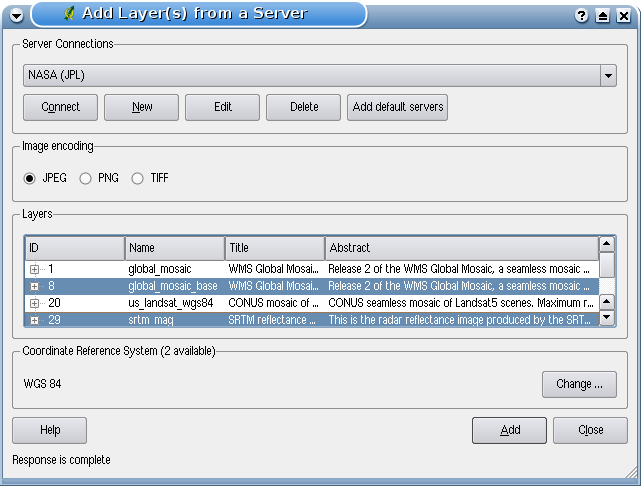
\includegraphics[clip=true,width=0.6\textwidth]{connection_wms}
  \end{center}
\end{figure}

\minisec{Image Encoding}

The \tab{Image encoding} section now lists the formats that are supported by both
the client and server.  Choose one depending on your image accuracy requirements.

\begin{Tip}[ht]\caption{\textsc{Image Encoding}}
\qgistip{You will typically find that a WMS server offers you the choice
of JPEG or PNG image encoding.  JPEG is a lossy compression format,
whereas PNG faithfully reproduces the raw raster data.

Use JPEG if you expect the WMS data to be photographic in nature and/or you don't
mind some loss in picture quality.  This trade-off typically reduces by 5 times
the data transfer requirement compared to PNG.

Use PNG if you want precise representations of the original data, and you don't mind
the increased data transfer requirements.
\index{WMS!image encoding}
}
\end{Tip}

\minisec{Layers}

The \tab{Layers} section lists the layers available from the selected
WMS server.  You may notice that some layers are expandible, this means
that the layer can be displayed in a choice of image styles.

You can select several layers at once, but only one image style per layer.
When several layers are selected, they will be combined at the WMS Server
and transmitted to QGIS in one go.

\begin{Tip}[ht]\caption{\textsc{WMS Layer Ordering}}
\qgistip{In this version of QGIS, WMS layers rendered by a server are overlaid
in the order listed in the Layers section, from top to bottom of the list.
If you want to overlay layers in the opposite order, then you can 
select \toolbtntwo{mActionAddWmsLayer}{Add WMS layer} a second time, choose the same server again,
and select the second group of layers that you want to overlay the first group.
\index{WMS!remote server!layer ordering}
}
\end{Tip}

\minisec{Transparency}
% BM: doesn't seem to work?
% \label{ogc-wms-transparency}
In this version of QGIS, the transparency setting is hard-coded to 
be always on, where available.  Therefore no option for it exists
on-screen.

This, in theory, allows you to overlay WMS layers on other layers (raster,
vector or WMS) and still see through to those lower layers.

\begin{Tip}[ht]\caption{\textsc{WMS Layer Transparency}}
\qgistip{The availability of WMS image transparency depends on
the image encoding used:  PNG and GIF support transparency,
whilst JPEG leaves it unsupported.
\index{WMS!layer transparency}
}
\end{Tip}

\minisec{Coordinate Reference System}
\index{WMS!CRS}\index{WMS!coordinate reference system}
\index{OGC!CRS}\index{OGC!coordinate reference system}
\index{Projections!WMS}
\index{Projections!CRS}\index{Projections!coordinate reference system}
\index{CRS}\index{coordinate reference system}

A Coordinate Reference System (CRS) is the OGC terminology for a QGIS Projection.

Each WMS Layer can be presented in multiple CRSs, depending
on the capability of the WMS server.  You may notice that the \textsl{x} changes in
the \textsl{Coordinate Reference System (x available)} header as you
select and deselect layers from the \tab{Layers} section.

To choose a CRS, select \button{Change...} and a screen similar to
Figure \ref{fig:projections} in Section \ref{label_projstart} will appear.
The main difference with the WMS version of the screen is that only
those CRSs supported by the WMS Server will be shown.


\begin{Tip}[ht]\caption{\textsc{WMS Projections}}
\qgistip{For best results, make the WMS layer the first layer
you add in the project.  This allows the project
projection to inherit the CRS you used to render the WMS layer.
On-the-fly projection (see Section \ref{sec:projection-specifying})
can then be used to fit any subsequent
vector layers to the project projection.
In this version of QGIS, if you add a WMS layer later, and give it a different
CRS to the current project projection, unpredictable
results can occur.
}
\end{Tip}


\subsubsection{Using the Identify Tool}\label{sec:ogc-wms-identify}
\index{WMS!identify}
\index{identify!WMS}

Once you have added a WMS server, 
and if any layer from a WMS server is queryable, you can then use
the \toolbtntwo{mActionIdentify}{Identify} tool to select a pixel on the map canvas.
A query is made to the WMS server for each selection made.

The results of the query are returned in plain text.
The formatting of this text is dependent on the particular
WMS server used.


\subsubsection{Viewing Properties}\label{sec:ogc-wms-properties}\index{WMS!properties}
\index{rasters!properties}

Once you have added a WMS server, you can view its properties
by right-clicking on it in the legend, and selecting
\button{Properties}.


\minisec{Metadata Tab}\label{sec:ogc-wms-properties-metadata}
\index{rasters!metadata}
\index{WMS!metadata}
\index{WMS!capabilites}

The \tab{Metadata} tab displays a wealth of information about the WMS server,
generally collected from the Capabilities statement returned from
that server.

Many definitions can be gleaned by reading the WMS
standards \cite{OGCWMS010101web}, \cite{OGCWMS010300web}, but
here are a few handy definitions:

\begin{itemize}
\item \textbf{Server Properties}

\begin{itemize}
\item \textbf{WMS Version}      - The WMS version supported by the server.

\item \textbf{Image Formats}    - The list of MIME-types the server can respond with when
                                  drawing the map.  QGIS supports whatever formats
                                  the underlying Qt libraries were built with, which
                                  is typically at least \texttt{image/png} 
                                  and \texttt{image/jpeg}.

\item \textbf{Identity Formats} - The list of MIME-types the server can respond with when
                                  you use the Identify tool.  Currently QGIS supports
                                  the \texttt{text-plain} type.

\end{itemize}

\item \textbf{Layer Properties}

\begin{itemize}
\item \textbf{Selected}         - Whether or not this layer was selected when its                                                                        server was added to this project.

\item \textbf{Visible}          - Whether or not this layer is selected as visible
                                  in the legend.  (Not yet used in this version of QGIS.)

\item \textbf{Can Identify}     - Whether or not this layer will return any results
                                  when the Identify tool is used on it.

\item \textbf{Can be Transparent} - Whether or not this layer can be rendered with transparency.
                                    This version of 
                                    QGIS will always use transparency if this is \textsl{Yes}
                                    and the image encoding supports transparency
% BM: doesn't seem to work?
%                                    (see Section
%                                    \ref{ogc-wms-transparency}
%                                    ).
                                    .

\item \textbf{Can Zoom In}      - Whether or not this layer can be zoomed in by the server.  This version
                                  of QGIS assumes all WMS layers have this set to \textsl{Yes}.
                                  Deficient layers may be rendered strangely.

\item \textbf{Cascade Count}    - WMS servers can act as a proxy to other WMS servers to get
                                  the raster data for a layer.  This entry shows how
                                  many times the request for this layer is forwarded to peer
                                  WMS servers for a result.

\item \textbf{Fixed Width}, \textbf{Fixed Height}
                                - Whether or not this layer has fixed source pixel dimensions.
                                  This version
                                  of QGIS assumes all WMS layers have this set to nothing.
                                  Deficient layers may be rendered strangely.

\item \textbf{WGS 84 Bounding Box} - The bounding box of the layer, in WGS 84 coordinates.
                                     Some WMS servers do not set this correctly (e.g. UTM
                                     coordinates are used instead).  If this is the case,
                                     then the initial view of this layer may be rendered
                                     with a very ``zoomed-out'' appearance by QGIS.
                                     The WMS webmaster should be informed of this error,
                                     which they may know as the WMS XML elements
                                     \texttt{LatLonBoundingBox},
                                     \texttt{EX\_GeographicBoundingBox} or
                                     the CRS:84 \texttt{BoundingBox}.

\item \textbf{Available in CRS} - The projections that this layer can be rendered in by
                                  the WMS server.  These are listed in the WMS-native format.

\item \textbf{Available in style} - The image styles that this layer can be rendered in by
                                    the WMS server.

\end{itemize}

\end{itemize}


\subsubsection{WMS Client Limitations}\label{sec:ogc-wms-limits}\index{WMS!client!limits}

Not all possible WMS Client functionality had been included in this version of QGIS.
Some of the more notable exceptions follow:

\minisec{Editing WMS Layer Settings}
\index{WMS!layer settings!editing}

Once you've completed the \toolbtntwo{mActionAddWmsLayer}{Add WMS layer}
procedure, there is no ability to change the settings.

A workaround is to delete the layer completely and start again.

\minisec{WMS Servers Requiring Authentication}
\index{WMS!remote server!authentication}

Only public WMS servers are accessible.
There is no ability to apply a user name and password combination
as an authentication to the WMS server.

\subsection{WFS Client}

In QGIS, a WFS layer behaves pretty much like any other vector layer. You 
can identify and select features and view the attribute table. The WFS 
plugin doesn't support editing at this time. 

Adding a WFS layer is very similar to the procedure used with WMS. The
difference is there are no default servers defined, so we have to add our
own.

\subsubsection{Loading a WFS Layer}

As an example we use the DM Solutions WFS server and display a layer. The URL is:
\begin{verbatim}
http://www2.dmsolutions.ca/cgi-bin/mswfs_gmap?VERSION=1.0.0&SERVICE=
wfs&REQUEST=GetCapabilities
\end{verbatim}

\begin{enumerate}
  \item Make sure the WFS plugin is loaded; if not, open the Plugin Manager and load it
  \item Click on the \toolbtntwo{wfs-icon}{Add WFS Layer} tool on the plugins toolbar
  \item Click on \button{New} 
  \item Enter \inputtext{Name}{DM Solutions} as the name
  \item Enter the URL (see previous page)
  \item Click \button{OK} 
  \item Choose \selectstring{Server Connections}{DM Solutions} from the drop-down box
  \item Click \button{Connect} 
  \item Wait for the list of layers to be populated
  \item Click on the \clicklistitem{Canadian Land} layer
  \item Click \button{Add} to add the layer to the map
  \item Wait patiently for the features to appear
\end{enumerate}

\begin{figure}[ht]
 \begin{center}
  \caption{Adding a WFS layer}\label{fig:wfs_dmsolutions}
  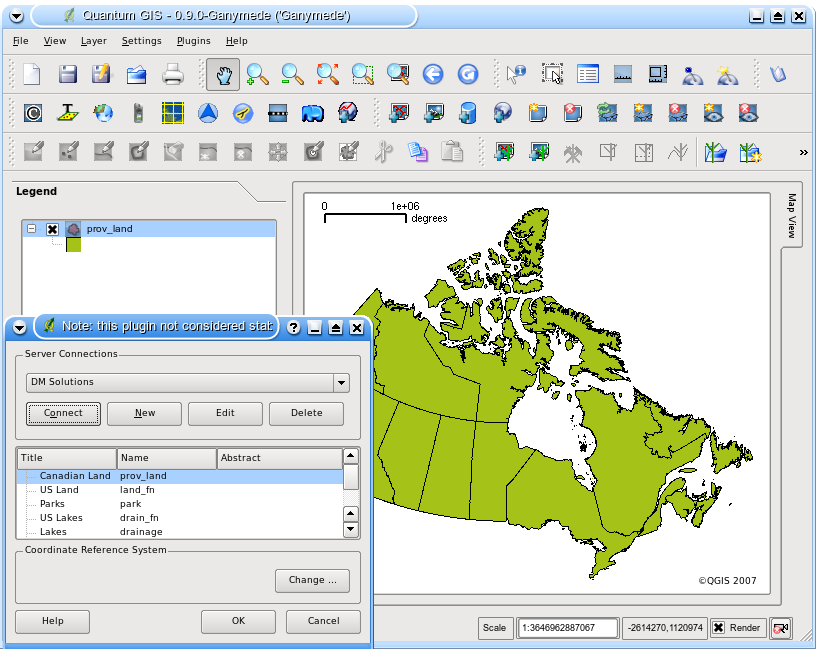
\includegraphics[clip=true,width=\textwidth]{wfs_dmsolutions}
 \end{center}
\end{figure}

You'll notice the download progress is visualized in the left bottom of the QGIS main window. 
Once the layer is loaded, you can identify and select a province or two and view the 
attribute table.

Remember this plugin works best with UMN MapServer WFS servers. It still
could be, that you might experience random behavior 
and crashes. You can look forward to improvements in a future version of the plugin.

\begin{Tip}[ht]\caption{\textsc{Finding WMS and WFS Servers}}
\qgistip{You can find additional WMS and WFS servers by using Google or your
favorite search engine. There are a number of lists, some of them
maintained and some not, that list public servers you can use.
\index{WFS!remote server!}
}
\end{Tip} 

%  !TeX  root  =  user_guide.tex

\chapter{QGIS Server}\label{label_qgisserver}
\index{WMS!QGIS Server}

% when the revision of a section has been finalized,
% comment out the following line:
% \updatedisclaimer

QGIS Mapserver это свободная реализация сервера WMS, совместимого со стандартом
WMS 1.3, которая кроме того имеет дополнительные возможности для тематического
картографирования. QGIS mapserver является написаным на С++ приложением FastCGI/CGI
(Common Gateway Interface), которое работает совместно с веб-сервером
(например, Apache или Lighttpd). Разработка сервера финансируется проектами
Orchestra ЕС, Sany и администрацией города Uster (Швейцария).

Он использует QGIS для отрисовки карты и ГИС-логики. Графическая подсистема
реализована при помощи библиотеки Qt, это же  позволило получить кроссплатформенность.
В отличие от других WMS-решений, QGIS Mapserver использует картографические
правила в SLD/SE и как язык конфигурирования сервера, и для описания пользовательских
картографических правил.

Кроме того, проект QGIS Mapserver предоставляет расширение <<Publish to Web>>
для QGIS, при помощи которого можно экспортировать текущие слои и символику
в проект для QGIS Mapserver (включая правила отображения в формате SLD).

Так как QGIS и QGIS mapserver используют одни и те же библиотеки визуализации,
карта, опубликованная в Интернет, выглядит точно так же, как и в настольной
ГИС. Модуль <<Publish to Web>> поддерживает базовую символику, более сложные
правила картографической визуализации задаются вручную. В качестве конфигурационных
файлов используется стандарт SLD и его расширения, таким образом, необходимо
знать только один стандартизированный язык, что значительно уменьшает сложность
создания карт для Интернет.

В следующих версиях руковдоства будет приведена инструкция по базовой
настройке сервера. В настоящее же время получить больше информации можно
по следующим ссылкам:

\begin{itemize}
\item \url{http://karlinapp.ethz.ch/qgis\_wms/}
\item \url{http://www.qgis.org/wiki/QGIS\_mapserver\_tutorial}
\item \url{http://linfiniti.com/2010/08/qgis-mapserver-a-wms-server-for-the-masses/}
\end{itemize}

\section{Пример установки на Debian Squeeze}

В этом разделе кратко описан процесс установки на Debian Squeeze. Бинарные
сборки существуют и для многих других операционных систем. Если вы скомпилировали
сервер WMS самостоятельно, обратитесь к ранее приведенным сайтам.

Кроме самой \qg и сервера WMS нужен еще и web-сервер, в нашем случае apache2.
Установить необходимые пакеты со всеми зависимостями можно при помощи
\usertext{aptitude} или \usertext{apt-get install}.

После установки необходимо убедиться, что и web-сервер, и сервер WMS работают
правильно.

Запустите web-сервер, выполнив команду \usertext{/etc/init.d/apache2 start}.
Откройте браузер и введите адрес: \url{http://localhost}. Если apache
запущен и работает правильно, в окне браузера отобразится текст <<It works!>>.

Теперь можно перейти к проверке работоспособности сервера WMS. Исполняемый
файл qgis\_mapserv.fcgi расположенный в \filename{/usr/lib/cgi-bin/qgis\_mapserv.fcgi}
является стандартным шаблоном WMS и отображает границы штатов США, как
показано на рисунке~\ref{fig:usa_wms}. Добавьте адрес \url{http://localhost/cgi-bin/qgis\_mapserv.fcgi}
к списку серверов WMS QGIS, как это описано в разделе~\ref{sec:ogc-wms-servers}.

\begin{figure}[ht]
\centering
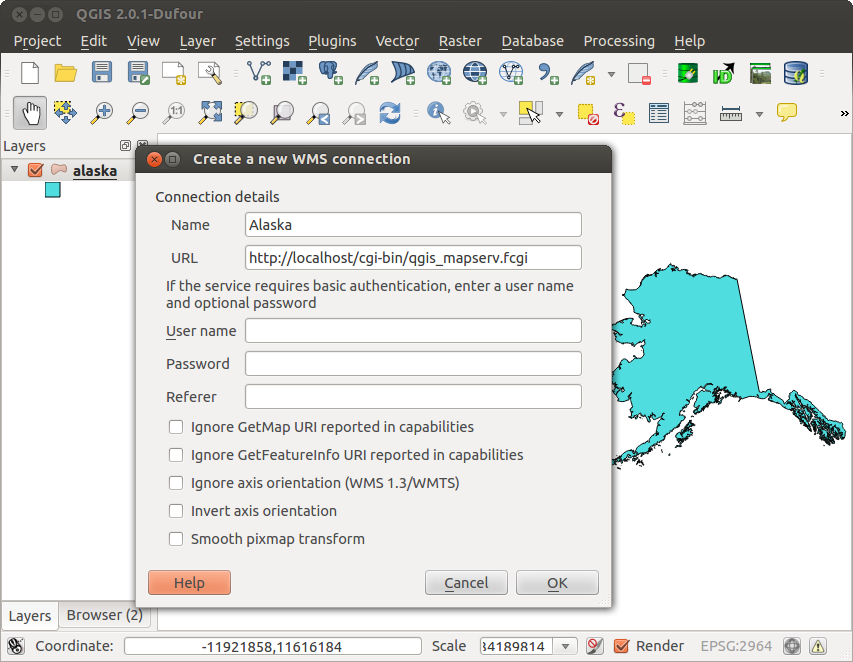
\includegraphics[clip=true, width=9cm]{standard_wms_usa}
\caption{Тестовый WMS с границами США из комплекта WMS сервера QGIS\nixcaption}
\label{fig:usa_wms}
\end{figure}

\section{Создание WMS на основе проекта QGIS}

Для создания нового сервера WMS нужно создать проект \qg и добавить в него
какие-то данные. В этом примере мы будем использовать shape-файлы <<regions>>
и <<aiport>> из демонстрационного набора данных \qg.

Сначала необходимо загрузить shape-файлы в проект, настроить цвета и стили
оформления слоёв, а также задать систему координат проекта. Затем вызовем
из меню \mainmenuopt{Установки} \arrow \mainmenuopt{Свойства проекта}
одноименное диалоговое окно и на вкладке \tab{Сервер WMS} заполним поля
<<Характеристики сервера>>, <<Достуные системы координат>> и <<Публикуемый
охват>>. При необходимости можно установить флажок
\checkbox{Включить WKT геометрию в ответ на GetFeatureInfo}, что сделает
возможным выполнение запросов к слою (см. Рисунок~\ref{fig:wmsdefinition}).
Сохраним проект как \filename{alaska\_airports.qgs}.

\begin{figure}[ht]
\centering
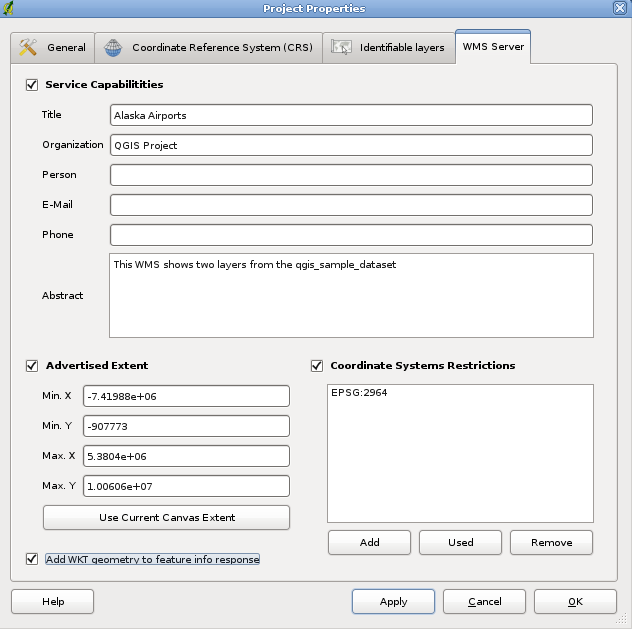
\includegraphics[clip=true, width=9cm]{wms_server_definition}
\caption{Характеристики проекта для сервера WMS \nixcaption}
\label{fig:wmsdefinition}
\end{figure}

Чтобы использовать сохраненный проект в качестве WMS, необходимо создать
новый подкаталог в каталоге \filename{/usr/lib/cgi-bin/project} (необходимы
привелегии суперпользователя), поместить в него файл проекта \filename{alaska\_airports.qgs}
и копию файла \filename{qgis\_mapserv.fcgi}.

Теперь можно проверить работу сервера, добавив его адрес
\url{http://localhost/cgi-bin/project/qgis\_mapserv.fcgi} в список серверов
WMS, как это описано в разделе~\ref{sec:ogc-wms-servers}. На рисунке~\ref{fig:wmsproject}
показана QGIS подключенная к серверу WMS на основе проекта.

\begin{figure}[ht]
\centering
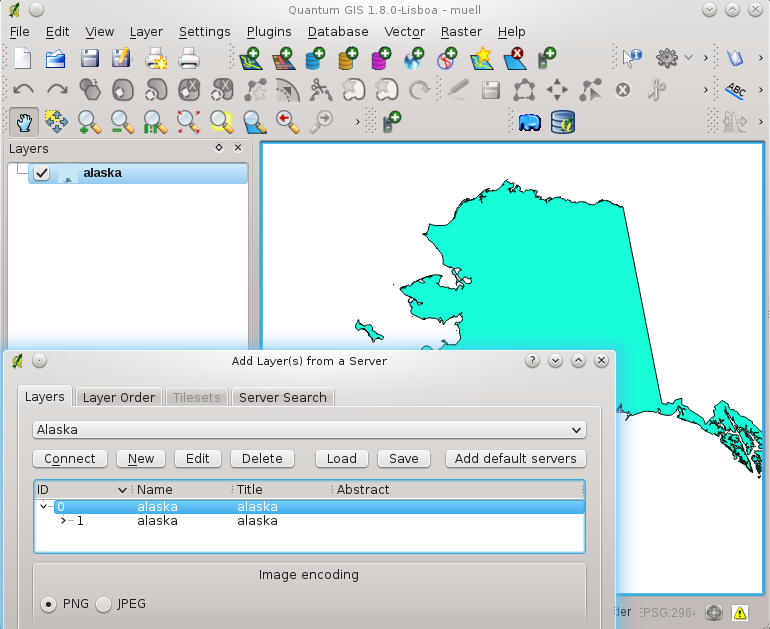
\includegraphics[clip=true, width=\textwidth]{wms_server_project}
\caption{Сервер WMS работающий на основе проекта QGIS \nixcaption}
\label{fig:wmsproject}
\end{figure}

\FloatBarrier

%  !TeX  root  =  user_guide.tex

\chapter{Working with Projections}\label{label_projections}
\index{Projections!working with}

% when the revision of a section has been finalized, 
% comment out the following line:
%\updatedisclaimer

QGIS allows users to define a global and project-wide CRS (Coordinate
Reference System) for layers without a pre-defined CRS. It also allows the
user to define custom coordinate reference systems and supports on-the-fly
(OTF) projection of vector layers. All these features allow the user to
display layers with different CRS and have them overlay properly.

\section{Overview of Projection Support}\label{label_projoverview}

QGIS has support for approximately 2,700 known CRS. Definitions for 
each of these CRS are stored in a SQLite database that is installed with
QGIS. Normally you do not need to manipulate the database directly. In fact,
doing so may cause projection support to fail. Custom CRS are stored in a
user database. See Section \ref{sec:customprojections} for
information on managing your custom coordinate reference systems.

The CRS available in QGIS are based on those defined by
EPSG\index{EPSG} and are largely abstracted from the spatial\_references 
table in PostGIS\index{PostGIS} version 1.x. The EPSG identifiers are
present in the database and can be used to specify a CRS in QGIS.

In order to use OTF projection, your data must contain information about its
coordinate reference system or you have to define a global, layer or
project-wide CRS. For PostGIS layers QGIS uses the spatial reference
identifier that was specified when the layer was created. For data supported
by OGR, QGIS relies on the presence of a format specific means of specifying
the CRS. In the case of shapefiles, this means a file containing the Well
Known Text (WKT)\index{WKT} specification of the CRS. The projection file
has the same base name as the shapefile and a prj extension. For example, a
shapefile named \filename{alaska.shp} would have a corresponding projection
file named \filename{alaska.prj}.

\section{Specifying a Projection}
\index{Projections!specifying}
\label{sec:projection-specifying}

QGIS no longer sets the map CRS to the coordinate reference system of the
first layer loaded. When you start a QGIS session with layers that do not
have a CRS, you need to control and define the CRS definition for these
layers. This can be done globally or project-wide in the \tab{CRS} tab under
\mainmenuopt{Edit} > \dropmenuopttwo{mActionOptions}{Options} (Gnome, OSX) 
or \mainmenuopt{Settings} > \dropmenuopttwo{mActionOptions}{Options} (KDE, Windows). 
See Figure~\ref{fig:crsdialog}. 

\begin{itemize}[label=--]
\item \checkbox{Prompt for CRS} 
\item \checkbox{Project wide default CRS will be used}
\item \checkbox{Global default CRS displayed below will be used}
\end{itemize}

The global default CRS \texttt{proj=longlat +ellps=WGS84 +datum=WGS84
+no\_defs} comes predefined in QGIS but can of course be changed, and the new
definition will be saved for subsequent QGIS sessions.    

\begin{figure}[ht]
   \centering
   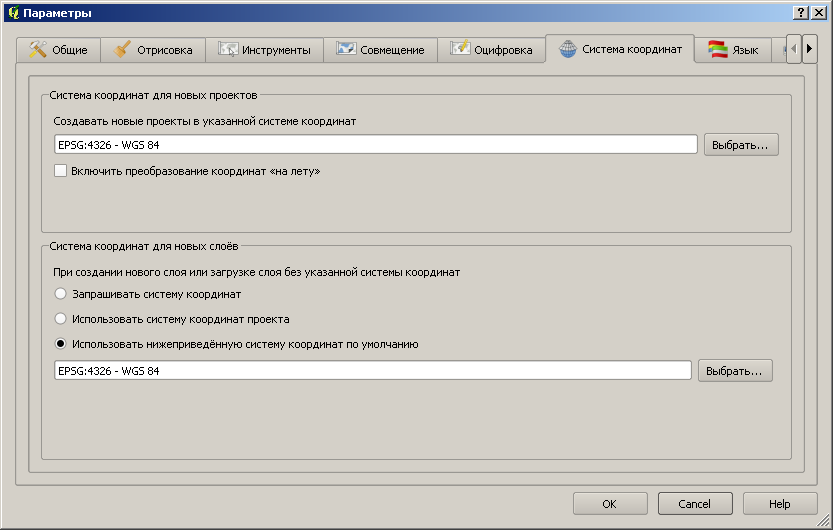
\includegraphics[clip=true, width=12cm]{crsdialog}
   \caption{CRS tab in the QGIS Options Dialog \nixcaption}\label{fig:crsdialog}
\end{figure}

If you want to define the coordinate reference system for a certain layer
without CRS information, you can also do that in the \tab{General} tab of the
raster (\ref{label_generaltab}) and vector (\ref{vectorgeneraltab}) properties 
dialog. If your layer already has a CRS defined, it
will be displayed as shown in Figure~\ref{fig:vector_symbology}.

\section{Define On The Fly (OTF) Projection}\label{label_projstart}

QGIS does not have OTF projection enabled by default, and this function is
currently only supported for vector layers. To use OTF projection, you must
open the \dropmenuopttwo{mActionOptions}{Project Properties} dialog, select a
CRS and activate the \checkbox{Enable on the fly projection} checkbox.
There are two ways to open the dialog:

\begin{enumerate}
\item Select \dropmenuopttwo{mActionOptions}{Project Properties} from the
\mainmenuopt{Edit} (Gnome, OSX) or \mainmenuopt{Settings} (KDE, Windows) menu.
\item Click on the \toolbtntwo{mIconProjectionDisabled}{projector} icon in the
lower right-hand corner of the statusbar.
\end{enumerate}

If you have already loaded a layer, and want to enable OTF projection, the
best practice is to open the \tab{Coordinate Reference System} tab of the
\dialog{Project Properties} dialog, select the CRS of the currently loaded
layer, and activate the \checkbox{Enable on the fly projection} checkbox. The
\toolbtntwo{mIconProjectionEnabled}{projector} icon will show a green hook
and all subsequently loaded vector layers will be OTF projected to the
defined CRS.
 
The \tab{Coordinate Reference System} tab of the \dialog{Project Properties}
dialog contains four important components as shown in Figure
\ref{fig:projections} and described below.

\begin{figure}[ht]
   \centering
   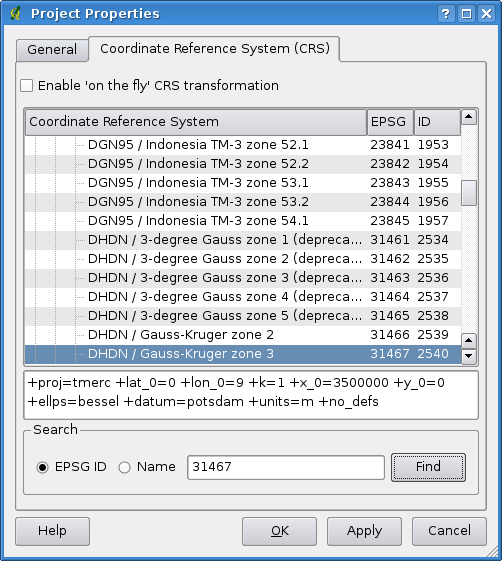
\includegraphics[clip=true, width=10cm]{projectionDialog}   
   \caption{Projection Dialog \nixcaption}\label{fig:projections}
\end{figure}

\begin{enumerate}
\item \textbf{Enable on the fly projection}\index{Projections!enabling} -
this checkbox is used to enable or disable OTF projection. When off, each
layer is drawn using the coordinates as read from the data source. When on,
the coordinates in each layer are projected to the coordinate reference
system defined for the map canvas.
\item \textbf{Coordinate Reference System} - this is a list of all CRS
supported by QGIS, including Geographic, Projected and Custom coordinate
reference systems. To use a CRS, select it from the list by expanding
the appropriate node and selecting the CRS. The active CRS is preselected.
\item \textbf{Proj4 text} - this is the CRS string used by the Proj4
projection engine. This text is read-only and provided for informational
purposes.
\item \textbf{Search} - if you know the EPSG identifier or the name 
for a Coordinate Reference System, you can use the search feature to find it.
Enter the identifier and click on \button{Find}.
\item \textbf{Recently used CRS} - if you have certain CRS that you frequently 
use in your everyday GIS work, these will be displayed as 'quick access' buttons 
at the bottom of the Projection Dialog. Click on one of these buttons to select 
the associated CRS.
\end{enumerate}

\begin{Tip}
\caption{\textsc{Project Properties Dialog}}
If you open the \dialog{Project Properties} dialog from the
\mainmenuopt{Edit} (Gnome, OSX) or \mainmenuopt{Settings} 
(KDE, Windows) menu, you must click on the \tab{Coordinate Reference
System} tab to view the CRS settings. Opening the dialog from the
\toolbtntwo{mIconProjectionEnabled}{projector} icon will automatically bring
the \tab{Coordinate Reference System} tab to the front.
\end{Tip}

\section{Custom Coordinate Reference System}\label{sec:customprojections}
\index{Projections!custom}

If QGIS does not provide the coordinate reference system you need, you
can define a custom CRS. To define a CRS, select
\dropmenuopttwo{mIconNew}{Custom CRS} from the \mainmenuopt{Edit} 
(Gnome, OSX) or \mainmenuopt{Settings} (KDE, Windows) menu.
Custom CRS are stored in your QGIS user database. In addition to your custom
CRS, this database also contains your spatial bookmarks and other custom data. 

\begin{figure}[ht]
   \centering
   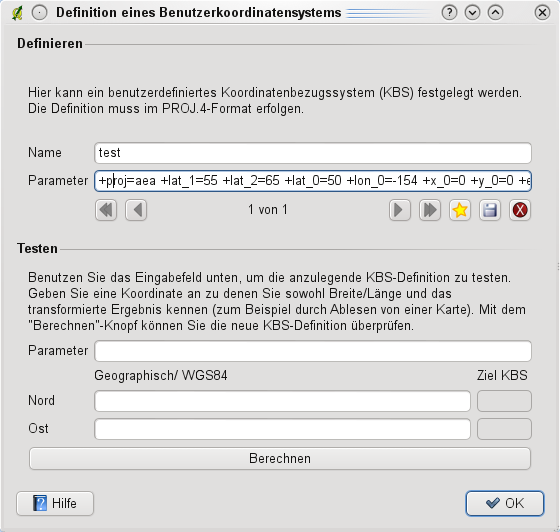
\includegraphics[clip=true, width=8cm]{customProjectionDialog}
   \caption{Custom CRS Dialog \nixcaption}\label{fig:customprojections}
\end{figure}

Defining a custom CRS in QGIS requires a good understanding of the Proj.4
projection library. To begin, refer to the Cartographic Projection Procedures
for the UNIX Environment - A User's Manual by Gerald I. Evenden, U.S.
Geological Survey Open-File Report 90-284, 1990 (available at \url{ftp://ftp.remotesensing.org/proj/OF90-284.pdf}).
This manual describes the use of the \usertext{proj.4} and related command line
utilities. The cartographic parameters used with \usertext{proj.4} are
described in the user manual, and are the same as those used by QGIS. 

The \dialog{Custom Coordinate Reference System Definition} dialog requires
only two parameters to define a user CRS: 
\begin{enumerate}
\item a descriptive name and
\item the cartographic parameters in PROJ.4 format.
\end{enumerate}
To create a new CRS, click the \toolbtntwo{mIconNew}{New} button and enter a
descriptive name and the CRS parameters. After that you can save your CRS by
clicking the button \toolbtntwo{mActionFileSave}{Save}.

Note that the \guilabel{Parameters} must begin with a \usertext{+proj=}-block,
to represent the new coordinate reference system.

You can test your CRS parameters to see if they give sane results by
clicking on the \button{Calculate} button inside the \guiheading{Test} block 
and pasting your CRS parameters into
the \guilabel{Parameters} field. Then enter known WGS 84 latitude and longitude
values in \guilabel{North} and \guilabel{East} fields respectively. 
Click on \button{Calculate} and compare the results with the known values in
your coordinate reference system.

\FloatBarrier

% vim: set textwidth=78 autoindent:

\section{GRASS GIS Integration}\label{sec:grass}\index{GRASS}

% when the revision of a section has been finalized, 
% comment out the following line:
%\updatedisclaimer

The GRASS plugin provides access to GRASS GIS~\cite{GRASSweb} databases and 
functionalities. This includes visualization of GRASS raster and vector 
layers, digitizing vector layers, editing vector attributes, creating new 
vector layers and analysing GRASS 2D and 3D data with more than 300 GRASS 
modules.

In this Section we'll introduce the plugin functionalities and give some 
examples on managing and working with GRASS data. Following main features 
are provided with the toolbar menu, when you start the GRASS plugin, as 
described in Section~\ref{sec:starting_grass}:
 
\begin{itemize}
\item \toolbtntwo{grass_open_mapset}{Open mapset}
\item \toolbtntwo{grass_new_mapset}{New mapset}
\item \toolbtntwo{grass_close_mapset}{Close mapset}
\item \toolbtntwo{grass_add_vector}{Add GRASS vector layer}
\item \toolbtntwo{grass_add_raster}{Add GRASS raster layer}
\item \toolbtntwo{grass_new_vector_layer}{Create new GRASS vector}
\item \toolbtntwo{grass_edit}{Edit GRASS vector layer}
\item \toolbtntwo{grass_tools}{Open GRASS tools}
%\item \toolbtntwo{grass_shell}{Open GRASS Shell}
\item \toolbtntwo{grass_region}{Display current GRASS region} 
\item \toolbtntwo{grass_region_edit}{Edit current GRASS region}
\end{itemize}

\subsection{Starting the GRASS plugin}\label{sec:starting_grass}
\index{GRASS!starting QGIS}

To use GRASS functionalities and/or visualize GRASS vector and raster layers 
in QGIS, you must select and load the GRASS plugin with the Plugin Manager. 
Therefore click the menu \mainmenuopt{Plugins} > \mainmenuopt{Manage Plugins}, 
select \dropmenuopt{GRASS} and click \button{OK}. 

You can now start loading raster and vector layers from an existing GRASS 
\filename{LOCATION} (see Section \ref{sec:load_grassdata}). Or you create a 
new GRASS \filename{LOCATION} with QGIS (see Section \ref{sec:create_loc}) 
and import some raster and vector data (see Section \ref{sec:import_loc_data}) 
for further analysis with the GRASS Toolbox (see Section 
\ref{subsec:grass_toolbox}).

\subsection{Loading GRASS raster and vector layers}\label{sec:load_grassdata}\index{GRASS!loading data}

With the GRASS plugin, you can load vector or raster layers using the
appropriate button on the toolbar menu. As an example we use the QGIS alaska
dataset (see Section \ref{label_sampledata}). It includes a small sample 
GRASS \filename{LOCATION} with 3 vector layers and 1 raster elevation map.

\begin{enumerate}
  \item Create a new folder \filename{grassdata}, download the QGIS alaska
  dataset \filename{qgis\_sample\_data.zip} from
  \url{http://download.osgeo.org/qgis/data/} and unzip the file into
  \filename{grassdata}. 
  \item Start QGIS.
  \item If not already done in a previous QGIS session, load the GRASS plugin
  clicking on \mainmenuopt{Plugins} > \mainmenuopt{Manage Plugins} and
  selecting \dropmenuopt{GRASS}. The GRASS toolbar appears on the toolbar menu.
  \item In the GRASS toolbar, click the \toolbtntwo{grass_open_mapset}{Open
  mapset} icon to bring up the \filename{MAPSET} wizard.
  \item For \filename{Gisdbase} browse and select or enter the path to the
  newly created folder \filename{grassdata}.
  \item You should now be able to select the \filename{LOCATION alaska}
  and the MAPSET \filename{demo}. 
  \item Click \button{OK}. Notice that some previously disabled tools in the 
  GRASS toolbar are now enabled.
  \item Click on \toolbtntwo{grass_add_raster}{Add GRASS raster layer},
  choose the map name \filename{gtopo30} and click \button{OK}. The elevation
  layer will be visualized.
  \item Click on \toolbtntwo{grass_add_vector}{Add GRASS vector layer},
  choose the map name \filename{alaska} and click \button{OK}. The alaska
  boundary vector layer will be overlayed on top of the gtopo30 map. You can
  now adapt the layer properties as described in chapter \ref{sec:vectorprops},
  e.g. change opacity, fill and outline color.
  \item Also load the other two vector layers \filename{rivers} and
  \filename{airports} and adapt their properties.
\end{enumerate}

As you see, it is very simple to load GRASS raster and vector layers in QGIS. 
See following Sections for editing GRASS data and creating a new 
\filename{LOCATION}. More sample GRASS \filename{LOCATIONs} are available at 
the GRASS website at \url{http://grass.osgeo.org/download/data.php}.

\begin{Tip}\caption{\textsc{GRASS Data Loading}}
\qgistip{If you have problems loading data or QGIS terminates abnormally,
check to make sure you have loaded the GRASS plugin properly as described in
Section \ref{sec:starting_grass}.
}
\end{Tip} 

\subsection{GRASS LOCATION and MAPSET}\label{sec:about_loc}

GRASS data are stored in a directory referred to as GISDBASE. This directory 
often called \filename{grassdata}, must be created before you start working 
with the GRASS plugin in QGIS. Within this directory, the GRASS GIS data 
are organized by projects stored in subdirectories called \filename{LOCATION}. 
Each \filename{LOCATION} is defined by its coordinate system, map projection 
and geographical boundaries. Each \filename{LOCATION} can have several 
\filename{MAPSETs} (subdirectories of the \filename{LOCATION}) that are used 
to subdivide the project into different topics, subregions, or as workspaces 
for individual team members (Neteler \& Mitasova 2008 
\cite{neteler_mitasova08}). In order to analyze vector and raster layers with 
GRASS modules, you must import them into a GRASS \filename{LOCATION}.
\footnote{This is not strictly true - with the GRASS modules 
\filename{r.external} and \filename{v.external} you can create read-only links 
to external GDAL/OGR-supported data sets without importing them. But because 
this is not the usual way for beginners to work with GRASS, this functionality 
will not be described here.}

\begin{figure}[ht]
\begin{center}
\caption{GRASS data in the alaska LOCATION (adapted from Neteler \& 
Mitasova 2008 \cite{neteler_mitasova08})}\label{fig:grass_location}\smallskip
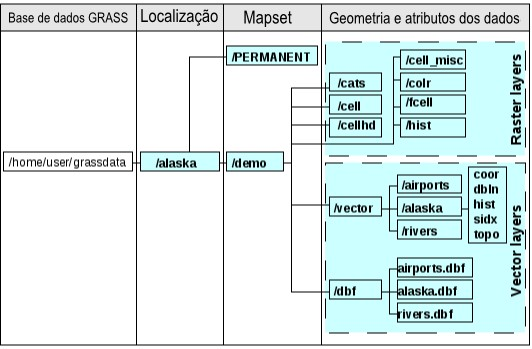
\includegraphics[clip=true]{grass_location}
\end{center}  
\end{figure}

\subsubsection{Creating a new GRASS LOCATION}\label{sec:create_loc}

As an an example you find the instructions how the sample GRASS
\filename{LOCATION alaska}, which is projected in Albers Equal Area
projection with unit feet was created for the QGIS sample dataset. This
sample GRASS \filename{LOCATION alaska} will be used for all examples and
exercises in the following GRASS GIS related chapters. It is useful to
download and install the dataset on your computer \ref{label_sampledata}).

\begin{figure}[ht]
\begin{center}
\caption{Creating a new GRASS LOCATION or a new MAPSET in QGIS \nixcaption}
\label{fig:create_grass_location}\smallskip
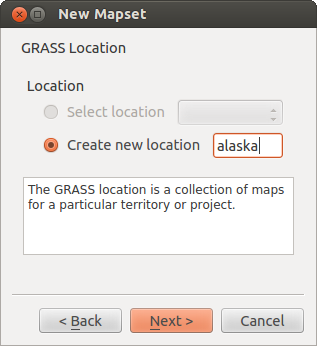
\includegraphics[clip=true, width=10cm]{create_grass_location}
\end{center}  
\end{figure}

\begin{enumerate}
  \item Start QGIS and make sure the GRASS plugin is loaded
  \item Visualize the \filename{alaska.shp} Shapefile (see Section
  \ref{sec:load_shapefile}) from the QGIS alaska dataset~\ref{label_sampledata}.
  \item In the GRASS toolbar, click on the \toolbtntwo{grass_open_mapset}{Open
    mapset} icon to bring up the \filename{MAPSET} wizard.
  \item Select an existing GRASS database (GISDBASE) folder 
  \filename{grassdata} or create one for the new \filename{LOCATION} using a 
  file manager on your computer. Then click \button{Next}. 
  \item We can use this wizard to create a new \filename{MAPSET} within an 
  existing \filename{LOCATION} (see Section~\ref{sec:add_mapset}) or to create 
  a new \filename{LOCATION} altogether. Click on the radio button
  \radiobuttonon{Create new location} (see Figure \ref{fig:create_grass_location}).
  \item Enter a name for the \filename{LOCATION} - we used alaska and click 
  \button{Next} 
  \item Define the projection by clicking on the radio button
  \radiobuttonon{Projection} to enable the projection list 
  \item We are using Albers Equal Area Alaska (feet) projection. Since we
  happen to know that it is represented by the EPSG ID 2964, we enter it in
  the search box. (Note: If you want to repeat this process for another 
  \filename{LOCATION} and projection and haven't memorized the EPSG ID, 
  click on the
  \toolbtntwo{mIconProjectionEnabled}{projector} icon in the lower right-hand
  corner of the status bar (see Section \ref{label_projstart})).
  \item Click \button{Find} to select the projection
  \item Click \button{Next} 
  \item To define the default region, we have to enter the \filename{LOCATION} 
  bounds in north, south, east, and west direction. Here we simply click on 
  the button \button{Set current QGIS extent}, to apply the extend of the 
  loaded layer \filename{alaska.shp} as the GRASS default region extend.
  \item Click \button{Next} 
  \item We also need to define a \filename{MAPSET} within our new 
  \filename{LOCATION}. You can name it whatever you like - we used demo.
  \footnote{When creating a new \filename{LOCATION}, GRASS automatically 
  creates a special \filename{MAPSET} called \filename{PERMANENT} designed to 
  store the core data for the project, its default spatial extend and 
  coordinate system definitions (Neteler \& Mitasova 2008 
  \cite{neteler_mitasova08}).}
  \item Check out the summary to make sure it's correct and click
  \button{Finish} 
  \item The new \filename{LOCATION alaska} and two \filename{MAPSETs demo}
  and \filename{PERMANENT} are created. The currently opened working set is
  \filename{MAPSET demo}, as you defined.
  \item Notice that some of the tools in the GRASS toolbar that were 
  disabled are now enabled.
\end{enumerate}

If that seemed like a lot of steps, it's really not all that bad and a very 
quick way to create a \filename{LOCATION}. The \filename{LOCATION alaska} is 
now ready for data import (see Section \ref{sec:import_loc_data}).
You can also use the already existing vector and raster data in the sample 
GRASS \filename{LOCATION alaska} included in the QGIS alaska dataset 
\ref{label_sampledata} and move on to Section \ref{label_vectmodel}.

\subsubsection{Adding a new MAPSET}\label{sec:add_mapset}

A user has only write access to a GRASS \filename{MAPSET} he created. This 
means, besides access to his own \filename{MAPSET}, each user can also read 
maps in other user's \filename{MAPSETs}, but he can modify or remove only 
the maps in his own \filename{MAPSET}. All \filename{MAPSETs} include a 
\filename{WIND} file that stores the current boundary coordinate values and 
the currently selected raster resolution (Neteler \& Mitasova 2008 
\cite{neteler_mitasova08}, see Section \ref{sec:grass_region}). 

\begin{enumerate}
  \item Start QGIS and make sure the GRASS plugin is loaded
  \item In the GRASS toolbar, click on the 
  \toolbtntwo{grass_new_mapset}{New mapset} icon to bring up the 
  \filename{MAPSET} wizard.
  \item Select the GRASS database (GISDBASE) folder \filename{grassdata} 
  with the \filename{LOCATION alaska}, where we want to add a further 
  \filename{MAPSET}, called test.
  \item Click \button{Next}. 
  \item We can use this wizard to create a new \filename{MAPSET} within an 
  existing \filename{LOCATION} or to create a new \filename{LOCATION} 
  altogether. Click on the radio button \radiobuttonon{Select location} 
  (see Figure \ref{fig:create_grass_location}) and click \button{Next}.
  \item Enter the name \filename{text} for the new \filename{MAPSET}. Below 
  in the wizard you see a list of existing \filename{MAPSETs} and its owners.
  \item Click \button{Next}, check out the summary to make sure it's all 
  correct and click \button{Finish} 
\end{enumerate}

\subsection{Importing data into a GRASS LOCATION}\label{sec:import_loc_data}

This Section gives an example how to import raster and vector data into the 
\filename{alaska} GRASS \filename{LOCATION} provided by the QGIS alaska 
dataset. Therefore we use a landcover raster map \filename{landcover.img} 
and a vector GML File \filename{lakes.gml} from the QGIS alaska 
dataset \ref{label_sampledata}.

\begin{enumerate}
  \item Start QGIS and make sure the GRASS plugin is loaded.
  \item In the GRASS toolbar, click the \toolbtntwo{grass_open_mapset}{Open 
  MAPSET} icon to bring up the \filename{MAPSET} wizard.
  \item Select as GRASS database the folder \filename{grassdata} in the QGIS 
  alaska dataset, as \filename{LOCATION alaska}, as \filename{MAPSET} 
  \filename{demo} and click \button{OK}.
  \item Now click the \toolbtntwo{grass_tools}{Open GRASS tools} icon. The 
  GRASS Toolbox (see Section \ref{subsec:grass_toolbox}) dialog appears.
  \item To import the raster map \filename{landcover.img}, click the module 
  \filename{r.in.gdal} in the \tab{Modules Tree} tab. This GRASS module 
  allows to import GDAL supported raster files into a GRASS 
  \filename{LOCATION}. The module dialog for \filename{r.in.gdal} appears.
  \item Browse to the folder \filename{raster} in the QGIS alaska dataset 
  and select the file \filename{landcover.img}.
  \item As raster output name define \filename{landcover\_grass} and click 
  \button{Run}. In the \tab{Output} tab you see the currently running GRASS 
  command \filename{r.in.gdal -o input=/path/to/landcover.img 
  output=landcover\_grass}.
  \item When it says \textbf{Succesfully finished} click \button{View output}. 
  The \filename{landcover\_grass} raster layer is now imported into GRASS and 
  will be visualized in the QGIS canvas.
  \item To import the vector GML file \filename{lakes.gml}, click the module 
  \filename{v.in.ogr} in the \tab{Modules Tree} tab. This GRASS module allows 
  to import OGR supported vector files into a GRASS \filename{LOCATION}. The 
  module dialog for \filename{v.in.ogr} appears.
  \item Browse to the folder \filename{gml} in the QGIS alaska 
  dataset and select the file \filename{lakes.gml} as OGR file.
  \item As vector output name define \filename{lakes\_grass} and click 
  \button{Run}. You don't have to care about the other options in this 
  example. In the \tab{Output} tab you see the currently running GRASS 
  command \filename{v.in.ogr -o dsn=/path/to/lakes.gml output=lakes\_grass}.
  \item When it says \textbf{Succesfully finished} click \button{View output}. 
  The \filename{lakes\_grass} vector layer is now imported into GRASS and will 
  be visualized in the QGIS canvas. 
\end{enumerate}


\subsection{The GRASS vector data model}\label{label_vectmodel}\index{GRASS!vector data
model}

It is important to understand the GRASS vector data model prior to
digitizing.\index{GRASS!digitizing} In general, GRASS uses a topological
vector model.\index{GRASS!topology} This means that areas are not represented
as closed polygons, but by one or more boundaries. A boundary between two
adjacent areas is digitized only once, and it is shared by both areas.
Boundaries must be connected without gaps. An area is identified (labeled) 
by the centroid of the area.

Besides boundaries and centroids, a vector map can also contain
points and lines. All these geometry elements can be mixed
in one vector and will be represented in different so called 'layers' inside
one GRASS vector map. So in GRASS a layer is not a vector or raster map but a
level inside a vector layer. This is important to distinguish carefully.
\footnote{Although it
is possible to mix geometry elements, it is unusual and even in GRASS only
used in special cases such as vector network analysis. Normally you should
prefere to store different geometry elements in different layers.}

It is possible to store more 'layers' in one vector dataset. For example,
fields, forests and lakes can be stored in one vector. Adjacent
forest and lake can share the same boundary, but they have separate attribute
tables. It is also possible to attach attributes to boundaries. For example,
the boundary between lake and forest is a road, so it can have a different 
attribute table.
 
The 'layer' of the feature is defined by 'layer' inside GRASS. 'Layer' is the 
number which defines if there are more than one layer inside the dataset, e.g. 
if the geometry is forest or lake. For now, it can be only a number, in the 
future GRASS will also support names as fields in the user interface.

Attributes can be stored inside the GRASS \filename{LOCATION} as DBase or 
SQLITE3 or in external database tables, for example PostgreSQL, MySQL, 
Oracle, etc.\index{GRASS!attribute storage}

Attributes in database tables are linked to geometry elements using
a 'category' value.\index{GRASS!attribute linkage} 'Category' (key, ID) is an
integer attached to geometry primitives, and it is used as the link to one
key column in the database table.

\begin{Tip}\caption{\textsc{Learning the GRASS Vector Model}}
\qgistip{
The best way to learn the GRASS vector model and its capabilities is to 
download one of the many GRASS tutorials where the vector model is described
more deeply. See \url{http://grass.osgeo.org/gdp/manuals.php} for more
information, books and tutorials in several languages.
}
\end{Tip} 

\subsection{Creating a new GRASS vector layer}\label{sec:creating_new_grass_vectors}\index{GRASS!Creating new vectors|see{editing!creating a new layer}}

To create a new GRASS vector layer with the GRASS plugin click the 
\toolbtntwo{grass_new_vector_layer}{Create new GRASS vector} toolbar icon. 
Enter a name in the text box and you can start digitizing point, line or 
polygone geometries, following the procedure described in Section 
\ref{grass_digitising}. 

In GRASS it is possible to organize all sort of geometry types (point, line 
and area) in one layer, because GRASS uses a topological vector model, so you 
don't need to select the geometry type when creating a new GRASS vector. This 
is different from Shapefile creation with QGIS, because Shapefiles use the 
Simple Feature vector model (see Section \ref{sec:create shape}).

\begin{Tip}\caption{\textsc{Creating an attribute table for a new GRASS vector layer}}
\qgistip{
If you want to assign attributes to your digitized geometry features, make sure to create an attribute table with columns before you start digitizing (see Figure \ref{fig:grass_digitizing_table}).
}
\end{Tip} 

\subsection{Digitizing and editing a GRASS vector layer}\index{GRASS!digitizing tools}\label{grass_digitising}

The digitizing tools for GRASS vector layers are accessed using the
\toolbtntwo{grass_edit}{Edit GRASS vector layer} icon on the toolbar. Make 
sure you have loaded a GRASS vector and it is the selected layer in the legend 
before clicking on the edit tool. Figure \ref{fig:grass_digitizing_category} 
shows the GRASS edit dialog that is displayed when you click on the edit tool. 
The tools and settings are discussed in the following sections.

\begin{Tip}\caption{\textsc{Digitizing polygones in GRASS}}
\qgistip{
If you want to create a polygone in GRASS, you first digitize the boundary of 
the polygone, setting the mode to \usertext{No category}. Then you add a 
centroid (label point) into the closed boundary, setting the mode to 
\usertext{Next not used}. The reason is, that a topological vector model links 
attribute information of a polygon always to the centroid and not to the 
boundary.
}
\end{Tip} 

\minisec{Toolbar}\label{label_grasstoolbar}

In Figure \ref{fig:grass_digitizing_toolbar} you see the GRASS digitizing
toolbar icons provided by the GRASS plugin. Table \ref{tab:grass_tools}
explains the available functionalities.

\begin{figure}[h]
   \begin{center}
   \caption{GRASS Digitizing Toolbar \nixcaption}\label{fig:grass_digitizing_toolbar} 
   
\includegraphics[clip=true,width=12cm]{grass_digitizing_toolbar}
\end{center}  
\end{figure}

\begin{table}[h]\index{GRASS!digitizing tools}
\centering
\caption{GRASS Digitizing Tools}\label{tab:grass_tools}\medskip
 \begin{tabular}{|l|l|p{5in}|}
 \hline \textbf{Icon} & \textbf{Tool} & \textbf{Purpose} \\
\hline 
\includegraphics[width=0.7cm]{grass_new_point} & New Point & Digitize
new point \\
\hline 
\includegraphics[width=0.7cm]{grass_new_line} & New Line & Digitize
new line (finish by selecting new tool) \\
\hline 
\includegraphics[width=0.7cm]{grass_new_boundary} & New Boundary &
Digitize new boundary (finish by selecting new tool)\\
\hline 
\includegraphics[width=0.7cm]{grass_new_centroid} & New Centroid &
Digitize new centroid (label existing area)\\
\hline 
\includegraphics[width=0.7cm]{grass_move_vertex} & Move vertex & Move
one vertex of existing line or boundary and identify new position\\
\hline 
\includegraphics[width=0.7cm]{grass_add_vertex} & Add vertex & Add a
new vertex to existing line\\
\hline 
\includegraphics[width=0.7cm]{grass_delete_vertex} & Delete vertex &
Delete vertex from existing line (confirm selected vertex by another click)\\
\hline \includegraphics[width=0.7cm]{grass_move_line} & Move element & Move
selected boundary, line, point or centroid and click on new position\\
\hline \includegraphics[width=0.7cm]{grass_split_line} & Split line & Split
an existing line to 2 parts\\
\hline \includegraphics[width=0.7cm]{grass_delete_line} & Delete element &
Delete existing boundary, line, point or centroid (confirm selected element by
another click)\\
\hline \includegraphics[width=0.7cm]{grass_edit_attributes} & Edit attributes
& Edit attributes of selected element (note that one element can represent
more features, see above)\\
\hline \includegraphics[width=0.7cm]{grass_close_edit} & Close & Close
session and save current status (rebuilds topology afterwards)\\
\hline
\end{tabular}
\end{table}

\minisec{Category Tab}\index{GRASS!category settings}

The \tab{Category} tab allows you to define the way in which the category 
values will be assigned to a new geometry element.

\begin{figure}[h]
 \begin{center}
  \caption{GRASS Digitizing Category Tab \nixcaption}\label{fig:grass_digitizing_category}
  \includegraphics[clip=true,width=10cm]{grass_digitizing_category}
 \end{center}
\end{figure}

\begin{itemize}
\item \textbf{Mode}: what category value shall be applied to new geometry 
elements.
\begin{itemize}
\item Next not used - apply next not yet used category value to geometry
element.
\item Manual entry - manually define the category value for the geometry
element in the 'Category'-entry field.
\item No category - Do not apply a category value to the geometry element.
This is e.g. used for area boundaries, because the category values are
connected via the centroid.
\end{itemize}
\item \textbf{Category} - A number (ID) is attached to each digitized geometry
element. It is used to connect each geometry element with its attributes.
\item \textbf{Field (layer)} - Each geometry element can be connected with
several attribute tables using different GRASS geometry layers. Default layer
number is 1. 
\end{itemize}

\begin{Tip}\caption{\textsc{Creating an additional GRASS 'layer' with QGIS}}
\qgistip{If you would like to add more layers to your dataset, just add a new
number in the 'Field (layer)' entry box and press return. In the Table tab
you can create your new table connected to your new layer.
}
\end{Tip}

\minisec{Settings Tab}\label{label_settingtab}\index{GRASS!snapping
tolerance}

The \tab{Settings} tab allows you to set the snapping in screen pixels. The
threshold defines at what distance new points or line ends are snapped to
existing nodes. This helps to prevent gaps or dangles between boundaries. The
default is set to 10 pixels.

\begin{figure}[h]
 \begin{center}
 \caption{GRASS Digitizing Settings Tab \nixcaption}\label{fig:grass_digitizing_settings}
 \includegraphics[clip=true,width=8cm]{grass_digitizing_settings}
 \end{center}
\end{figure}

\minisec{Symbology Tab}\index{GRASS!symbology settings}

The \tab{Symbology} tab allows you to view and set symbology and color
settings for various geometry types and their topological status (e.g. closed
/ opened boundary).

\begin{figure}[h]
 \begin{center}
 \caption{GRASS Digitizing Symbolog Tab \nixcaption}\label{fig:grass_digitizing_symbology}
 \includegraphics[clip=true,width=8cm]{grass_digitizing_symbology}
 \end{center}
\end{figure}

\minisec{Table Tab} \index{GRASS!table editing}

The \tab{Table} tab provides information about the database table for
a given 'layer'. Here you can add new columns to an existing attribute table,
or create a new database table for a new GRASS vector layer (see Section 
\ref{sec:creating_new_grass_vectors}).

\begin{figure}[h]
 \begin{center}
 \caption{GRASS Digitizing Table Tab \nixcaption}\label{fig:grass_digitizing_table}
 \includegraphics[clip=true,width=10cm]{grass_digitizing_table}
 \end{center}
\end{figure}

\begin{Tip}\caption{\textsc{GRASS Edit Permissions}}\index{GRASS!edit
permissions}
\qgistip{You must be the owner of the GRASS \filename{MAPSET} you want to 
edit. It is impossible to edit data layers in a \filename{MAPSET} that is not 
yours, even if you have write permissions.
}
\end{Tip} 

\subsection{The GRASS region tool}\label{sec:grass_region}\index{GRASS!region}

The region definition (setting a spatial working window) in GRASS is important 
for working with raster layers. Vector analysis is per default not limited
to any defined region definitions. All newly-created rasters will have the
spatial extension and resolution of the currently defined GRASS region,
regardless of their original extension and resolution. The current GRASS
region is stored in the \filename{\$LOCATION/\$MAPSET/WIND} file, and it 
defines north, south, east and west bounds, number of columns and rows, 
horizontal and vertical spatial resolution.

It is possible to switch on/off the visualization of the GRASS region in the
QGIS canvas using the \toolbtntwo{grass_region}{Display current GRASS region}
button. \index{GRASS!region!display}.

With the \toolbtntwo{grass_region_edit}{Edit current GRASS region} icon you 
can open a dialog to change the current region and the symbology of the GRASS 
region rectangle in the QGIS canvas. Type in the new region bounds and 
resolution and click \button{OK}. It also allows to select a new region 
interactively with your mouse on the QGIS canvas. Therefore click with the 
left mouse button in the QGIS canvas, open a rectangle, close it using the 
left mouse button again and click \button{OK}.\index{GRASS!region!editing}
The GRASS module \filename{g.region} provide a lot more parameters to define 
an appropriate region extend and resolution for your raster analysis. You can 
use these parameters with the GRASS Toolbox, described in Section 
\ref{subsec:grass_toolbox}.

\subsection{The GRASS toolbox}\label{subsec:grass_toolbox}\index{GRASS!toolbox}

The \toolbtntwo{grass_tools}{Open GRASS Tools} box provides GRASS module 
functionalities to work with data inside a selected GRASS \filename{LOCATION} 
and \filename{MAPSET}. To use the GRASS toolbox you need to open a 
\filename{LOCATION} and \filename{MAPSET} where you have write-permission 
(usually granted, if you created the \filename{MAPSET}). This is necessary, 
because new raster or vector layers created during analysis need to be written 
to the currently selected \filename{LOCATION} and \filename{MAPSET}.

\subsubsection{Working with GRASS modules}\index{GRASS!toolbox}

\begin{figure}[h]
\centering
\caption{GRASS Toolbox and searchable Modules List \nixcaption}\label{fig:grass_modules}
   \subfigure[Modules Tree] {\label{subfig:grass_module_tree}\includegraphics[clip=true, width=0.4\textwidth]{grass_toolbox_moduletree}}\goodgap
   \subfigure[Searchable Modules List] {\label{subfig:grass_module_list}\includegraphics[clip=true, width=0.4\textwidth]{grass_toolbox_modulelist}}
\end{figure}

The GRASS Shell inside the GRASS Toolbox provides access to almost all (more 
than 300) GRASS modules in command line modus. To offer a more user
friendly working environment, about 200 of the available GRASS modules and 
functionalities are also provided by graphical dialogs. These dialogs are 
grouped in thematic blocks, but are searchable as well. You find a complete 
list of GRASS modules available in QGIS version \CURRENT
in appendix \ref{appdx_grass_toolbox_modules}. It is also possible to 
customize the GRASS Toolbox content. It is described in Section 
\ref{sec:toolbox-customizing}.

As shown in Figure \ref{fig:grass_modules}, you can look for the appropriate 
GRASS module using the thematically grouped \tab{Modules Tree} or the 
searchable \tab{Modules List} tab. 

Clicking on a grapical module icon a new tab will be added to the toolbox 
dialog providing three new sub-tabs \tab{Options}, \tab{Output} and 
\tab{Manual}. In Figure \ref{fig:grass_module_dialog} you see an example 
for the GRASS module \filename{v.buffer}.

\begin{figure}[h]
\centering
\caption{GRASS Toolbox Module Dialogs \nixcaption}\label{fig:grass_module_dialog}
   \subfigure[Module Options] {\label{subfig:grass_module_option}\includegraphics[clip=true, width=0.3\textwidth]{grass_module_option}}\goodgap
   \subfigure[Modules Output] {\label{subfig:grass_module_output}\includegraphics[clip=true, width=0.3\textwidth]{grass_module_output}}\goodgap
   \subfigure[Module Manual] {\label{subfig:grass_module_manual}\includegraphics[clip=true, width=0.3\textwidth]{grass_module_manual}}
\end{figure}

\minisec{Options}

The \tab{Options} tab provides a simplified module dialog where you can 
usually select a raster or vector layer visualized in the QGIS canvas and 
enter further module specific parameters to run the module. The provided 
module parameters are often not complete to keep the dialog clear. If you want 
to use further module parameters and flags, you need to start the GRASS Shell 
and run the module in the command line.

\minisec{Output}

The \tab{Output} tab provides information about the output status of the 
module. When you click the \button{Run} button, the module switches to the 
\tab{Output} tab and you see information about the analysis process. If all 
works well, you will finally see a \usertext{Successfully finished} message.

\minisec{Manual}

The \tab{Manual} tab shows the HTML help page of the GRASS module. You can 
use it to check further module parameters and flags or to get a deeper 
knowledge about the purpose of the module. At the end of each module 
manual page you see further links to the \filename{Main Help index}, the 
\filename{Thematic index} and the \filename{Full index}. These links provide 
the same information as if you use the module \filename{g.manual} 

\begin{Tip}\caption{\textsc{Display results immediately}}\index{GRASS!display results}
\qgistip{If you want to display your calculation results immediately in your 
map canvas, you can use the 'View Output' button at the bottom of the 
module tab.
}
\end{Tip} 

\subsubsection{Working with the GRASS LOCATION browser} \index{GRASS!toolbox!Browser}

Another useful feature inside the GRASS Toolbox is the GRASS 
\filename{LOCATION} browser. In Figure~\ref{fig:grass_mapset_browser} you 
can see the current working \filename{LOCATION} with its \filename{MAPSETs}.

In the left browser windows you can browse through all \filename{MAPSETs} 
inside the current \filename{LOCATION}. The right browser window shows some 
meta information for selected raster or vector layers, e.g. resolution, 
bounding box, data source, connected attribute table for vector data and a 
command history.

\begin{figure}[h]
 \begin{center}
 \caption{GRASS LOCATION browser \nixcaption}\label{fig:grass_mapset_browser}
 \includegraphics[clip=true,width=10cm]{grass_mapset_browser}
 \end{center}
\end{figure}

The toolbar inside the \tab{Browser} tab offers following tools to manage 
the selected \filename{LOCATION}:

\begin{itemize}
\item \toolboxtwo{grass_add_map}{Add selected map to canvas}
\item \toolboxtwo{grass_copy_map}{Copy selected map}
\item \toolboxtwo{grass_rename_map}{Rename selected map}
\item \toolboxtwo{grass_delete_map}{Delete selected map}
\item \toolboxtwo{grass_set_region}{Set current region to selected map}
\item \toolboxtwo{grass_refresh}{Refresh browser window}
\end{itemize}

The \toolboxtwo{grass_rename_map}{Rename selected map} and 
\toolboxtwo{grass_delete_map}{Delete selected map} only work with maps inside 
your currently selected \filename{MAPSET}. All other tools also work with 
raster and vector layers in another \filename{MAPSET}.

\subsubsection{Customizing the GRASS Toolbox} \index{GRASS!toolbox!customize}
\label{sec:toolbox-customizing}

Nearly all GRASS modules can be added to the GRASS toolbox. A XML 
interface is provided to parse the pretty simple XML files which configures 
the modules appearance and parameters inside the toolbox.

A sample XML file for generating the module \usertext{v.buffer} (v.buffer.qgm) 
looks like this:
\begin{verbatim}
<?xml version="1.0" encoding="UTF-8"?>
<!DOCTYPE qgisgrassmodule SYSTEM "http://mrcc.com/qgisgrassmodule.dtd">

<qgisgrassmodule label="Vector buffer" module="v.buffer">
        <option key="input" typeoption="type" layeroption="layer" />
        <option key="buffer"/>
        <option key="output" />
</qgisgrassmodule>
\end{verbatim}

The parser reads this definition and creates a new tab inside the toolbox 
when you select the module. A more detailed description for adding new 
modules, changing the modules group, etc. can be found on the QGIS wiki at \\
\url{http://wiki.qgis.org/qgiswiki/Adding\_New\_Tools\_to\_the\_GRASS\_Toolbox}.


% vim:autoindent:set textwidth=78:

\section{Print Composer}\label{label_printcomposer}

% when the revision of a section has been finalized, 
% comment out the following line:
\updatedisclaimer

The print composer provides growing layout and printing
capabilities. It allows you to add elements such as the QGIS map canvas, 
legend, scalebar, images, and text labels. You can size, group 
and position each element and adjust the properties to create your layout. 
The result can be printed (also to Postscript and PDF), exported as an image, 
or exported to SVG.\footnote{Export to SVG is currently not supported, 
because this functionality is not working with recent QT4 versions.} See a
list of all buttons in table~\ref{tab:printcomposer_tools} below:

\begin{table}[h]\index{Print composer!tools}
\centering
\caption{Print Composer Tools}\label{tab:printcomposer_tools}\medskip
 \begin{tabular}{|l|p{6.9cm}|l|p{6.9cm}|}
 \hline \textbf{Icon} & \textbf{Purpose} & \textbf{Icon} &
 \textbf{Purpose} \\

 \hline \includegraphics[width=0.7cm]{mActionExportMapServer}
 & Export to an image format & 
 \includegraphics[width=0.7cm]{mActionSaveAsSVG} & Export print composition 
 to SVG \\
 \hline \includegraphics[width=0.7cm]{mActionFilePrint} & Print or 
 export as PDF or Postscript &
 \includegraphics[width=0.7cm]{mActionZoomFullExtent} & Zoom to
 full extend \\
 \hline \includegraphics[width=0.7cm]{mActionZoomIn} & Zoom in &
 \includegraphics[width=0.7cm]{mActionZoomOut} & Zoom out \\
 \hline \includegraphics[width=0.7cm]{mActionDraw} & Refresh 
 view &
 \includegraphics[width=0.7cm]{mActionAddRasterLayer} & Add 
 new map from QGIS map canvas \\
 \hline \includegraphics[width=0.7cm]{mActionSaveMapAsImage} & Add Image to 
 print composition &
 \includegraphics[width=0.7cm]{mActionLabel} & Add label to print composition \\
 \hline \includegraphics[width=0.7cm]{mActionAddLegend} & Add new legend to 
 print composition & 
 \includegraphics[width=0.7cm]{mActionScaleBar} & Add new scalebar to print
 composition\\
 \hline \includegraphics[width=0.7cm]{mActionSelectPan} & Select/Move item in 
 print composition &
 \includegraphics[width=0.7cm]{mActionMoveItemContent} & Move content within
 an item \\
 \hline \includegraphics[width=0.7cm]{mActionGroupItems} & Group items of 
 print composition & 
 \includegraphics[width=0.7cm]{mActionUngroupItems} & Ungroup items of print 
 composition \\
 \hline \includegraphics[width=0.7cm]{mActionRaiseItems} & Raise selected
 items in print composition &
 \includegraphics[width=0.7cm]{mActionLowerItems} & Lower selected items 
 in print composition \\
 \hline \includegraphics[width=0.7cm]{mActionMoveItemsToTop} & Move selected
 items to top & 
 \includegraphics[width=0.7cm]{mActionMoveItemsToBottom} & Move selected
 items to bottom \\
\hline
\end{tabular}
\end{table}

To access the print composer, click on the \toolbtntwo{mActionFilePrint}{Print}
button in the toolbar or choose \mainmenuopt{File} > \dropmenuopttwo{mActionFilePrint}{Print}.

\subsection{Using Print Composer}\label{label_useprintcomposer} 

To use the print composer, first add the layers you
want to print to QGIS. The layers should be rendered and symbolized to your
liking prior to composing the map (see example in Figure \ref{fig:print_composer_complete}). 

\begin{figure}[ht]
   \begin{center}
   \caption{Print Composer}\label{fig:print_composer_blank}\smallskip
   \includegraphics[clip=true, width=\textwidth]{print_composer_blank}
\end{center}  
\end{figure}

Opening the print composer provides you with a blank canvas to which you can add
the current map view, legend, scalebar, and text. Figure
\ref{fig:print_composer_blank} shows the initial view of the print composer before
any elements are added.

The print composer has two tabs: \tab{General} and \tab{Item}. The General tab
allows you to set the paper size, orientation, and resolution for the map.
The Item tab displays the properties for the currently selected map element.
By selecting an element on the map (eg. legend, scalebar, text, etc.) and
clicking on the \tab{Item} tab, you can customize the settings.

You can add multiple elements to the composer. This allows you to have more
than one map view and legend in the composer. Each element has its own
properties and in the case of the map, its own extent.

\subsubsection{Adding a map layout to the Print Composer}

To add the QGIS map canvas to the print composer, click on the
%FIXME \toolbtntwo{composer_add_image}{Add a new map} 
button in toolbar. Drag a rectangle on the composer canvas to add the
map. You can resize the map later by clicking on the \button{Select/move item}
button, clicking on the map, and dragging one of the handles in the corner of
the map. With the map selected, you can also resize the map by specifying the
width and height on the Item properties tab.

The map is linked to the QGIS map canvas. If you change the view on the map
canvas by zooming or panning, you can update the print composer view by
selecting the map in the print composer and clicking on the \button{Set Extent} 
button. You can also change the print composer view by specifying a map scale. 
To set the view to a specific scale:

\begin{enumerate}
\item Choose \selectstring{Set}{Scale (calculate extent)}
\item Enter the scale denominator in the scale box
\item Press Enter
\end{enumerate} 

\subsubsection{Adding other Elements to the Print Composer} 
 
Already existing QGIS templates can be used to easily load and adapt print
layouts. To open an existing template, click on the
%FIXME \toolbtntwo{composer_open_template}{Open Template} 
button. Choose a template and
customize its appearance. 

To add a logo, north arrow or any  kind of image to the composer, click on
the 
%FIXME \toolbtntwo{composer_add_image}{Add Image} 
button. The image will 
be placed on the composer canvas and you can move it where you like. 

A legend can be added to the composer canvas and customized to show only the
desired layers. To add a legend, click on the
%FIXME \toolbtntwo{composer_add_legend08}{Add Vector Legend} 
button. The legend will be
placed on the composer canvas and you can move it where you like. Click on
the \tab{Items} tab to customize the appearance of the legend, including
which layers are shown.

To add a scalebar to the composer, click on the
%FIXME \toolbtntwo{composer_add_scalebar08}{Add Scalebar} 
button. Use the \tab{Item}
tab to customize the segment size, number of segments, scalebar units, size,
and font for the scalebar.

You can add text labels to the composer by clicking on the
%FIXME \toolbtntwo{composer_add_label}{Add New Label} 
button. Use the \tab{Item} tab
while the text is selected to customize the settings or change the default text.

Figure \ref{fig:print_composer_complete} shows the print composer after adding
each type of map element.
\begin{figure}[h]
   \begin{center}
   \caption{Print Composer with map view, legend, scalebar, and text added}
   \label{fig:print_composer_complete}\smallskip
   \includegraphics[clip=true, width=\textwidth]{print_composer_complete}
\end{center}  
\end{figure}

\subsubsection{Other Features}

The print composer has navigation tools to zoom in and out. To zoom in, click
the \button{Zoom in} tool. The print composer canvas will be scaled by a factor to 2. Use
the scrollbars to adjust the view to the area of interest. Zooming out works
in a similar fashion.

If you find the view in an inconsistent state, you can use the \button{Refresh} button
to redraw the print composer canvas.

\subsubsection{Creating Output}

The print composer allows you to print the layout to a printer, export to a PNG or
export to SVG. Each of these functions is available from the composer toolbar.

To save the composer canvas as a templates, click on the
%\toolbtntwo{composer_save_template}{Save Template As} 
button. Browse to the directory 
you like and save a template to use it again for another map canvas.

It is possible to export the result as an image by clicking on the
%FIXME \toolbtntwo{composer_export_image}{Export as image} 
button. 

To export the composer canvas as an  SVG (Scalable Vector Graphic), click on
the 
%FIXME \toolbtntwo{composer_export_svg}{Export as SVG} 
button. \textbf{Note:}
Currently the SVG output is very basic. This is not a QGIS problem, but a
problem of the underlaying Qt library. This will be sorted out in future versions.
 

%first the general intro to plugins
%then each individual plugin can have a section
%in the plugins chapter
\section{Using Plugins}\index{plugins}

%% FIXME: here we need to include new python plugin section and updates

\subsection{An Introduction to Using Plugins}\label{label_introplugin}

QGIS has been designed with a plugin architecture.
This allows new features/functions to be added to the application.
Many of the features in QGIS are actually implemented as plugins.

There are two types of plugins in QGIS: core and user-contributed.
\index{plugins!types} A core plugin is maintained by the QGIS development team and is part of every QGIS distribution.
A user-contributed plugin is an external plugin that is maintained by the individual author.
The QGIS SVN website (\url{http://svn.qgis.org}) serves some user contributed plugins.

\subsubsection{Finding and Installing a Plugin}
When you install QGIS, all of the core plugins are included (see chapter \ref{sec:core_plugins}). \index{plugins!installing}
% Additional user-contributed
% plugins may be available on the QGIS Community site. To see what
% user-contributed plugins are available, see the plugins page on the Community
% site (\url{http://community.qgis.org/plugins}).\index{plugins!user
% contributed}

Typically user-contributed plugins are distributed in source form and require compiling.
For instructions on building and installing a user-contributed plugin, see the documentation included with the plugin.

\subsubsection{Managing Plugins}\label{sec:managing_plugins}
\index{plugins!managing} Managing plugins consists of loading or unloading them from QGIS.
Loaded plugins are "remembered" when you exit the application and restored the next time you run QGIS.

To manage plugins, open \mainmenuopt{Plugins} > \dropmenuopttwo{mActionShowPluginManager}{Plugin Manager...}
\index{plugins!manager}The Plugin Manager displays all the available plugins and their status (loaded or unloaded).
Figure \ref{fig:pluginmanager} shows the Plugin Manager dialog.

%\begin{figure}[ht]
%   \begin{center}
%   \caption{Plugin Manager}\label{fig:pluginmanager}\smallskip
%   \includegraphics[clip=true, width=14cm]{pluginmanager2}
%\end{center}  
%\end{figure}

Typically all QGIS plugins are installed in the same location.
This location is shown in the Plugin Directory text field.
You can tell QGIS to load plugins from another location by specifying a different directory.

\begin{Tip}\caption{\textsc{Crashing Plugins}}\index{crashes}
\qgistip{If you find that QGIS crashes on startup, a plugin may be at fault.
You can stop all plugins from loading by editing your stored settings file (see \ref{subsec:gui_options} for location).
Locate the plugins settings and change all the plugin values to false to prevent them from loading.
\nix {For example, to prevent the Delimited text plugin from loading, the entry in \$HOME/.config/QuantumGIS/qgis.conf on Linux 
should look like this:\ttfamily{Add Delimited Text Layer=false}.}
\normalfont 
Do this for each plugin in the [Plugins] section.
You can then start QGIS and add the plugins one at a time from the Plugin Manger to determine which is causing the problem.
}
\end{Tip} 

\subsubsection{Data Providers}\index{data providers}

Data Providers are "special" plugins that provides access to a data store.
By default, QGIS supports PostGIS layers and disk-based data stores supported by the GDAL/OGR library (Appendix \ref{appdx_ogr}).
A Data Provider plugin extends the ability of QGIS to use other data sources.

Data Provider plugins are registered automatically by QGIS at startup.
They are not managed by the Plugin Manager but are used behind the scenes when a corresponding data type is added as a layer in QGIS.

\subsubsection{Core Plugins}\label{sec:core_plugins}\index{plugins!core}

QGIS currently contains 11 core plugins that can be loaded using the Plugin Manager.
Table \ref{tab:core_plugins} lists each of the core plugins along with a description of their purpose and the toolbar-icon.
Note the GRASS plugin is not included below because it installs its own toolbar (see section \ref{sec:grass} for a discussion of available features in the GRASS plugin).

% minipage is needed to appear the footnote under the table
% SH
\begin{minipage}{\textwidth}
\begin{table}[H]
\centering
\caption{QGIS Core Plugins}\label{tab:core_plugins}\medskip
\small
 \begin{tabular}{|l|l|p{4in}|}
\hline \textbf{Icon} & \textbf{Plugin} & \textbf{Description} \\
\hline 
% WHICH ICON TO CHOOSE HERE?
\includegraphics[width=0.7cm]{delimited_text}
 & Delimited Text \index{plugins!delimited text}& Load a delimited text file containing x,y coordinates as a point layer \\
\hline 
\includegraphics[width=0.7cm]{copyright_label}
 & Copyright Label \index{plugins!copyright}& Display a copyright label on the map canvas\\
\hline 
\includegraphics[width=0.7cm]{gps_importer}
 & GPS Tools \index{plugins!gps}& Load and display GPS data \\
\hline
\includegraphics[width=0.7cm]{georeferencer}
 & Georeferencer \index{plugin!georeferencer} & Georeferencing rasterlayers \\
\hline
\includegraphics[width=0.7cm]{grid_maker}
 & Graticule Creator \index{plugins!graticule}& Create a latitude/longitude grid and save as a shapefile\\
\hline
\includegraphics[width=0.7cm]{north_arrow}
& North Arrow \index{plugins!north arrow}& Add a north arrow to the map canvas\\
\hline
\includegraphics[width=0.7cm]{icon_buffer}
 & PostgreSQL Geoprocessing \index{plugins!geoprocessing}& Buffer a PostGIS layer \\
\hline
\includegraphics[width=0.7cm]{quick_print}
 & Quick Print \index{plugins!quickprint}& Quickly print a map \\
\hline
\includegraphics[width=0.7cm]{spit}
 & SPIT \index{plugins!spit}& Shapefile to PostGIS Import Tool - import shapefiles into PostgreSQL\\
\hline
\includegraphics[width=0.7cm]{scale_bar}
 & Scalebar \index{plugins!scalebar}& Add a scalebar to the map canvas\\
\hline 
\includegraphics[width=0.7cm]{mIconAddWfsLayer}
 & WFS & Load and display WFS layer \\
\hline
\end{tabular}
\end{table}
\end{minipage}

\normalsize


\begin{Tip}\caption{\textsc{Plugins Settings Saved to Project}}\index{plugins
settings}
\qgistip{When you save a .qgs project, any changes you have made to NorthArrow, ScaleBar and Copyright plugins will be saved in the project and restored next time you load the project.
}
\end{Tip}

%
% External Plugins
%
\subsubsection{External Plugins}\label{sec:external_plugins}\index{plugins!external}

QGIS also comes with some externally developed plugins.
They are not shipped with the default distribution.
However, they can be compiled and used within QGIS.

Currently the external plugins are only available directly from SVN.
To check out all available external plugins do the following:
\begin{verbatim}
svn co https://svn.osgeo.org/qgis/trunk/external_plugins external_qgis_plugins
\end{verbatim}

This will create a folder \texttt{external\_qgis\_plugins} in your current folder.
Each subdirectory has its own compile and install instructions.
Read them carefully in order to build the plugin.

%
% Plugin template
%
\subsubsection{Plugin templates}\label{sec:plugin_template}\index{plugins!template}

If you like to develop your own QGIS-plugin the main sources include a nice script which guides you through the process of creating your own template-directory-structure within the QGIS-source-tree.
The script lives in \texttt{QGIS/src/plugins/plugin\_builder.pl}.

The only thing to do is coding your functions into the plugin (and of course contribute your plugin to the QGIS-development-team).

Beside that the QGIS-wiki (\url{http://wiki.qgis.org}) and the QGIS-blog (\url{http://blog.qgis.org}) provide useful articles about writing your own plugin as well.
Check the websites for details!

\section{Using QGIS Core Plugins}\label{sec:core_plugins}\index{plugins!core}

QGIS currently contains 11 core plugins that can be loaded using the Plugin Manager.
Table \ref{tab:core_plugins} lists each of the core plugins along with a description of their purpose and the toolbar-icon.
Note the GRASS plugin is not included below because it installs its own toolbar (see section \ref{sec:grass} for a discussion of available features in the GRASS plugin).

% minipage is needed to appear the footnote under the table
% SH
\begin{minipage}{\textwidth}
\begin{table}[H]
\centering
\caption{QGIS Core Plugins}\label{tab:core_plugins}\medskip
\small
 \begin{tabular}{|l|l|p{4in}|}
\hline \textbf{Icon} & \textbf{Plugin} & \textbf{Description} \\
\hline 
% WHICH ICON TO CHOOSE HERE?
\includegraphics[width=0.7cm]{delimited_text}
 & Delimited Text \index{plugins!delimited text}& Load a delimited text file containing x,y coordinates as a point layer \\
\hline 
\includegraphics[width=0.7cm]{copyright_label}
 & Copyright Label \index{plugins!copyright}& Display a copyright label on the map canvas\\
\hline 
\includegraphics[width=0.7cm]{gps_importer}
 & GPS Tools \index{plugins!gps}& Load and display GPS data \\
\hline
\includegraphics[width=0.7cm]{georeferencer}
 & Georeferencer \index{plugin!georeferencer} & Georeferencing rasterlayers \\
\hline
\includegraphics[width=0.7cm]{grid_maker}
 & Graticule Creator \index{plugins!graticule}& Create a latitude/longitude grid and save as a shapefile\\
\hline
\includegraphics[width=0.7cm]{north_arrow}
& North Arrow \index{plugins!north arrow}& Add a north arrow to the map canvas\\
\hline
\includegraphics[width=0.7cm]{icon_buffer}
 & PostgreSQL Geoprocessing \index{plugins!geoprocessing}& Buffer a PostGIS layer \\
\hline
\includegraphics[width=0.7cm]{quick_print}
 & Quick Print \index{plugins!quickprint}& Quickly print a map \\
\hline
\includegraphics[width=0.7cm]{spiticon}
 & SPIT \index{plugins!spit}& Shapefile to PostGIS Import Tool - import shapefiles into PostgreSQL\\
\hline
\includegraphics[width=0.7cm]{scale_bar}
 & Scalebar \index{plugins!scalebar}& Add a scalebar to the map canvas\\
\hline 
\includegraphics[width=0.7cm]{mIconAddWfsLayer}
 & WFS & Load and display WFS layer \\
\hline
\end{tabular}
\end{table}
\end{minipage}

\normalsize


\begin{Tip}\caption{\textsc{Plugins Settings Saved to Project}}\index{plugins
settings}
\qgistip{When you save a .qgs project, any changes you have made to NorthArrow, ScaleBar and Copyright plugins will be saved in the project and restored next time you load the project.
}
\end{Tip}



\subsection{Using the Coordinate Capture Plugin}

% when the revision of a section has been finalized, 
% comment out the following line:
% \updatedisclaimer

The coordinate capture plugin is easy to use and provides the 
capability to display coordinates on the map canvas for two 
selected Coordinate Reference Systems (CRS). You can click a 
certain point and copy the coordinates to the clipboard or you 
use the mouse tracking functionality 

\begin{figure}[ht]
   \begin{center}
   \caption{Coordinate Cature Plugin \nixcaption}\label{fig:coordinate_capture_dialog}\smallskip
   \includegraphics[clip=true]{coordinate_capture_dialog}
\end{center}  
\end{figure}

\begin{enumerate}
  \item Start QGIS, select \dropmenuopttwo{mActionOptions}{Project Properties} from 
  the \mainmenuopt{Settings} menu and click on the \tab{Projection} tab. As an alternative you 
  you can also click on the \toolbtntwo{mIconProjectionEnabled}{projector} icon in the lower 
  right-hand corner of the statusbar.
  \item Click on the \checkbox{Enable on the fly projection} checkbox and select the projected 
  coordinate system \filename{"NAD27/Alaska Albers"} with EPSG 2964 (see also 
  Section \ref{label_projections}).
  \item Load the \filename{alaska.shp} vector layer from the qgis sample dataset.
  \item Load the coordinate capture plugin in the Plugin Manager (see Section 
  \ref{sec:load_core_plugin}) and click on the \toolbtntwo{coordinate_capture}{Coordinate Capture} 
  icon. The cordinate capture dialog appears as shown in Figure \ref{fig:coordinate_capture_dialog}.
  \item Click on the \toolbtntwo{geographic}{Click to the select the CRS to use for coordinate display} 
  icon and select Geographic Coordinate System \filename{WGS84} (EPSG 4326).
  \item You can now click anywhere on the map canvas and the plugin will show the 
  \filename{"NAD27/Alaska Albers"} and \filename{WGS84} coordinates for your selected points as shown in 
  Figure \ref{fig:coordinate_capture_dialog}.
  \item To enable mouse coordinate tracking click the \toolbtntwo{tracking}{mouse tracking} icon.
  \item You can also copy selected coordinates to the clipboard.
\end{enumerate}

\newpage




%  !TeX  root  =  user_guide.tex

\section{Decorations Plugins}

% when the revision of a section has been finalized,
% comment out the following line:
\updatedisclaimer

The Decorations Plugins includes the Copyright Label Plugin, the North
Arrow Plugin and the Scale Bar Plugin. They are used to ``decorate'' the
map by adding cartographic elements.

\subsection{Copyright Label Plugin}\label{copyrightlabel}

The title of this plugin is a bit misleading - you can add any random text to the map.

\begin{figure}[ht]
   \centering
   \includegraphics[clip=true, width=7cm]{copyright}
   \caption{Copyright Label Plugin \nixcaption}\label{fig:copyright}
\end{figure}

\begin{enumerate}
\item Make sure the plugin is loaded
\item Click on \mainmenuopt{Plugins} \arrow \dropmenuopt{Decorations} \arrow \dropmenuopttwo{copyright_label}{Copyright Label} or use the \toolbtntwo{copyright_label}{Copyright Label} button from the Toolbar.
\item Enter the text you want to place on the map. You can use HTML as
  shown in the example
\item Choose the placement of the label from the \selectstring{Placement}{Bottom Right} drop-down box
\item Make sure the \checkbox{Enable Copyright Label} checkbox is checked
\item Click \button{OK}
\end{enumerate}

In the example above (default) places a copyright symbol followed by the date in the
lower right hand corner of the map canvas.

\subsection{North Arrow Plugin}\label{northarrow}

The North Arrow plugin places a simple north arrow on the map canvas. At
present there is only one style available. You can adjust the angle of the
arrow or let QGIS set the direction automatically. If you choose to let
QGIS determine the direction, it makes its best guess as to how the arrow
should be oriented. For placement of the arrow you have four options,
corresponding to the four corners of the map canvas.

\begin{figure}[ht]
   \centering
   \includegraphics[clip=true, width=8cm]{north_arrow_dialog}
   \caption{North Arrow Plugin \nixcaption}\label{fig:north_arrow}
\end{figure}

\subsection{Scale Bar Plugin}\label{scalebar}

The Scale Bar plugin adds a simple scale bar to the map canvas. You
control the style and placement, as well as the labeling of the bar.

QGIS only supports displaying the scale in the same units as your map frame. So
if the units of your layers are in meters, you can't create a scale bar in
feet. Likewise if you are using decimal degrees, you can't create a scale
bar to display distance in meters.

To add a scale bar:

\begin{enumerate}
\item Click on \mainmenuopt{Plugins} \arrow \dropmenuopt{Decorations} \arrow \dropmenuopttwo{scale_bar}{Scale Bar} or use the \toolbtntwo{scale_bar}{Scale Bar} button from the Toolbar.
\item Choose the placement from the \selectstring{Placement}{Bottom Left} drop-down list
\item Choose the style from the \selectstring{Scale bar style}{Tick Down} list
\item Select the color for the bar \selectcolor{Color of bar}{black} or use the default black color
\item Set the size of the bar and its label \selectnumber{Size of bar}{30 degrees}
\item Make sure the \checkbox{Enable scale bar} checkbox is checked
\item Optionally choose to automatically snap to a round number when the
  canvas is resized \checkbox{Automatically snap to round number on resize}
\item Click \button{OK}
\end{enumerate}

\begin{figure}[ht]
   \centering
   \includegraphics[clip=true, width=8cm]{scale_bar_dialog}
   \caption{Scale Bar Plugin \nixcaption}\label{fig:scale_bar}
\end{figure}

\begin{Tip}\caption{\textsc{Plugins Settings Saved to Project}}\index{plugins settings}
When you save a .qgs project, any changes you have made to NorthArrow, ScaleBar and Copyright plugins will be saved in the project and restored nexttime you load the project.
\end{Tip}

\FloatBarrier

\subsection{Using the Delimited Text Plugin}\label{label_dltext}    

% when the revision of a section has been finalized, 
% comment out the following line:
\updatedisclaimer

The Delimited Text plugin allows you to load a delimited text file as a layer in QGIS. 
    
\subsubsection{Requirements}

To view a delimited text file as layer, the text file must contain:

\begin{enumerate}      
\item A delimited header row of field names. This must be the first line in the text file.
\item The header row must contain an X and Y field. These fields can have any name.
\item The x and y coordinates must be specified as a number. The coordinate system is not important.
\end{enumerate}

An example of a valid text file might look like this:

\begin{verbatim} 
name|latdec|longdec|cell|
196 mile creek|61.89806|-150.0775|tyonek d-1 ne|
197 1/2 mile creek|61.89472|-150.09972|tyonek d-1 ne|
a b mountain|59.52889|-135.28333|skagway c-1 sw|
apw dam number 2|60.53|-145.75167|cordova c-5 sw|
apw reservoir|60.53167|-145.75333|cordova c-5 sw|
apw reservoir|60.53|-145.75167|cordova c-5 sw|
aaron creek|56.37861|-131.96556|bradfield canal b-6|
aaron island|58.43778|-134.81944|juneau b-3 ne|
aats bay|55.905|-134.24639|craig d-7|
\end{verbatim}


Some items of note about the text file are:

\begin{enumerate}        
\item  The example text file uses \mbox{$|$} as delimiter. Any character can be used to delimit the fields.
\item The first row is the header row. It contains the fields name, latdec, longdec and cell.
\item No quotes ({\tt{}"{}}) are used to delimit text fields.
\item The x coordinates are contained in the {\em longdec} field.
\item The y coordinates are contained in the {\em latdec} field.
\end{enumerate}

\subsubsection{Using the Plugin}
To use the plugin you must have QGIS running and use the Plugin Manager to load the plugin:

Start QGIS, then open the Plugin Manager by choosing \mainmenuopt{Plugins} > \dropmenuopttwo{mActionShowPluginManager}{Plugin Manager...}
\index{plugins!manager}
The Plugin Manager displays a list of available plugins.
Those that are already loaded have a check mark to the left of their name.
Click on the checkbox to the left of the \checkbox{Add Delimited Text Layer} plugin and click \button{OK} to load it as described in Section \ref{sec:managing_plugins}.


A new toolbar icon is now present:
\includegraphics[width=0.7cm]{delimited_text}
Click on the icon \toolbtntwo{delimited_text}{Add Delimited Text Layer} to open the Delimited Text dialog as shown in Figure
\ref{fig:delim_text_plugin_dialog}.

%\begin{figure}[ht]
%   \begin{center}
%   \caption{Delimited Text
%Dialog}\label{fig:delim_text_plugin_dialog}\smallskip
%\includegraphics[clip=true, width=8cm]{dialog}            
%   \end{center}  
%\end{figure}

First select the file to import by clicking on the \browsebutton .
Select the desired text file from the file dialog.
Once the file is selected, the plugin attempts to parse the file using the last used delimiter, in this case \mbox{$|$} (see Figure \ref{fig:delim_text_file_selected}).

%\begin{figure}[ht]
%   \begin{center}
%   \caption{File Selected}\label{fig:delim_text_file_selected}\smallskip
%\includegraphics[clip=true, width=8cm]{file_selected}   
%   \end{center}  
%\end{figure}
  
In this case the delimiter \mbox{$|$} is not correct for the file.
The file is actually tab delimited.
Note that the X and Y field drop down boxes do not contain valid field names.

%\begin{figure}[ht]
%   \begin{center}
%   \caption{Fields Parsed from Text
%File}\label{fig:delim_text_file_selected2}\smallskip  
%\includegraphics[clip=true, width=8cm]{file_selected2}
%   \end{center}  
%\end{figure}

To properly parse the file, change the delimiter to tab using \mbox{$\backslash$}t (this is a regular expression for the tab character).
After changing the delimiter, click \button{Parse}.
The drop down boxes now contain the fields properly parsed as shown in Figure \ref{fig:delim_text_file_selected2}.

%\begin{figure}[ht]
%   \begin{center}
%   \caption{Selecting the X and Y
%Fields}\label{fig:delim_text_file_selected3}\smallskip
%\includegraphics[clip=true, width=8cm]{file_selected3}
%   \end{center}  
%\end{figure}

Choose the X and Y fields from the drop down boxes and enter a Layer name as shown in Figure \ref{fig:delim_text_file_selected3}.
To add the layer to the map, click \button{Add Layer}.
The delimited text file now behaves as any other map layer in QGIS.
\subsection{Dxf2Shp Converter Plugin}

% when the revision of a section has been finalized, 
% comment out the following line:
\updatedisclaimer

The dxf2shape converter plugin allows to convert vector data from DXF to Shapefile 
format. It is very simple to handle and provides following functionality as 
shown in Figure \ref{fig:dxf2shape_dialog}.

\begin{itemize}
\item \textbf{Input DXF file}: Enter path to the DXF file to be converted
\item \textbf{Output Shp file}: Enter desired name of the shape file to be created
\item \textbf{Output file type}: specifies the type of the output Shapefile. Currently supported is polyline, polygone and point.
\item \textbf{Export text labels}: If you enable this checkbox, an additional Shapefile points layer will be created, and the associated dbf table will contain information about the "TEXT" fields found in the dxf file, and the text strings themselves.
\end{itemize}

\begin{figure}[ht]
   \begin{center}
   \caption{Dxf2Shape Converter Plugin \nixcaption}\label{fig:dxf2shape_dialog}\smallskip
   \includegraphics[clip=true, width=13cm]{dxf2shape_dialog}
\end{center}  
\end{figure}

\begin{enumerate}
  \item Start QGIS, load the Dxf2Shape plugin in the Plugin Manager (see Section 
  \ref{sec:load_core_plugin}) and click on the \toolbtntwo{dxf2shp_converter}{Dxf2Shape Converter} 
  icon which appears in the QGIS toolbar menu. The Dxf2Shape plugin dialog appears as shown in Figure \ref{fig:dxf2shape_dialog}.
  \item Enter input DXF file, a name for the output Shapefile and the Shapefile type.
  \item Enable the \checkbox{Export text labels} checkbox, if you want to create an extra point layer with labels.
  \item Click \button{Ok}. 
\end{enumerate}

\newpage




% vim: set textwidth=78 autoindent:

\subsection{eVis Plugin}\label{sec:evis}

The Biodiversity Informatics Facility at the American Museum of Natural History's (AMNH) Center 
for Biodiversity and Conservation (CBC) \footnote{This section is derived from Horning, N., K.
Koy, P. Ersts. 2009. eVis (v1.1.0) User's Guide. American Museum of
Natural History, Center for Biodiversity and Conservation. Available from
\url{http://biodiversityinformatics.amnh.org/}, and released under the GNU FDL.} has developed the
Event Visualization Tool (eVis), 
another software tool to add to the suite of conservation monitoring and decision support tools 
for guiding protected area and landscape planning. This plugin enables users to easily link 
geocoded (i.e., referenced with latitude and longitude or X and Y coordinates) photographs, 
and other supporting documents, to vector data in QGIS.

eVis is now automatically installed and enabled in new versions of QGIS, and as with all plugins, 
it can be disabled and enabled using the Plugin Manager (See Section \ref{sec:managing_plugins}).

The eVis plugin is made up of three modules: the Database Connection tool, Event ID tool, and 
the Event Browser. These work together to allow viewing of geocoded photographs and other documents 
that are linked to features stored in vector files, databases, or spreadsheets.

\subsubsection{Event Browser}\label{evis_browser}

The Event Browser module provides the functionality to display geocoded photographs that are linked
to vector features displayed in the QGIS map window. Point data, for example, can be from a vector
file that can be input using QGIS or it can be from the result of a database query. The vector
feature must have attribute information associated with it to describe the location and name of the
file containing the photograph and, optionally, the compass direction the camera was pointed when
the image was acquired. Your vector layer must be loaded into QGIS before running the Event Browser.

\minisec{Launch the Event Browser module}\label{evis_launch_browser}

To launch the Event browser module either click on the \toolbtntwo{event_browser}{Event Browser}
icon or click on \mainmenuopt{Plugins} > \dropmenuopt{eVis} >
\dropmenuopt{eVis Event Browser}. This will open the Generic Event Browser window.

The Generic Event Browser window has three tabs displayed at the top of the window. The Display tab
is used to view the photograph and its associated attribute data. The Options tab provides a number
of settings that can be adjusted to control the behavior of the eVis plugin. Lastly, the Configure
External Applications tab is used to maintain a table of file extensions and their associated
application to allow eVis to display documents other than images.

\minisec{Understanding the Display window}\label{evis_display_window}

To see the Display window click on the \tab{Display} tab in the Generic Event Browser
window. The Display window is used to view geocoded photographs and their associated attribute data.

\begin{figure}[ht]
   \begin{center}
\caption{\label{evisdisplay}The \emph{eVis} display window \nixcaption}
\includegraphics[clip=true, width=12cm]{evisdisplay}
\end{center}
\end{figure}

\begin{itemize}
\item \textbf{Display window}: A window where the photograph will appear.
\item \textbf{Increase zoom button}: Zoom in to see more detail. If the entire image cannot be
displayed in the display window, scroll bars will appear on the left and bottom sides of the window
to allow you to pan around the image.
\item \textbf{Reduce zoom button}: Zoom out to see more area. 
\item \textbf{Zoom to full extent button}: Displays the full extent of the photograph.
\item \textbf{Attribute information window}: All of the attribute information for the point
associated with the photograph being viewed is displayed here. If the file type being referenced in
the displayed record is not an image but is of a file type defined in the Configure External
Applications tab then when you double-click on the value of the field containing the path to the
file the application to open the file will be launched to view or hear the contents of the file. If
the file extension is recognized the attribute data will be displayed in green.
\item \textbf{Navigation buttons}: Use the Previous and Next buttons to load the previous or next
feature when more than one feature is selected.
\item \textbf{Feature indicator}: This heading indicates which feature is being displayed and how
many features are available for display.
\end{itemize}

\minisec{Understanding the Options window}\label{evis_options_window}

\begin{figure}[ht]
   \begin{center}
\caption{\label{evisoptions}The \emph{eVis} Options window \nixcaption}
\includegraphics[clip=true, width=12cm]{evisoptions}
\end{center}
\end{figure}

\begin{itemize}
\item \textbf{File location}: A dropdown list to specify the attribute field that contains the
directory path or URL for the photographs or other documents being displayed. If the location is a
relative path then the checkbox to the right of the dropdown menu must be clicked. The base path for
a relative path can be entered in the Base Path text box below. Information about the different
options for specifying the file location are noted in the section 4.5 below.
\item \textbf{Compass bearing display field}: A dropdown list to specify the attribute field
that contains the compass bearing associated with the photograph being displayed. If compass bearing
information is available it is necessary to click the radio button to the left of the dropdown menu
title.
\item \textbf{Compass offset setting}: Compass offsets can be used to compensate for
declination (adjust bearings collected using magnetic bearings to true north bearings). Click the
Manual radio-button to enter the offset in the text box or click the From Attribute  radio-button to
select the attribute field containing the offsets. For both of these options east declinations
should be entered using positive values and west declinations should use negative values.
\item \textbf{Directory base path}: The base path onto which the relative path defined in
Figure \ref{evisoptions} (A) will be appended.
\item \textbf{Replace path}: If this check-box is checked, only the file name from the A
will be appended to the Base Path.
\item \textbf{Apply rule to all documents}: If checked, the same path rules that are defined
for photographs will be used for non-image documents such as movies, text documents, and sound
files. If not checked the path rules will only apply to photographs and other documents will ignore
the Base Path  parameter.
\item \textbf{Save settings}: If the check-box is checked the values for the associated
parameters will be saved for the next session when the window is closed or when the Save button
below is pressed.
\item \textbf{Reset values}: Resets the values on this line to the default setting.
\item \textbf{Restore faults}: This will reset all of the fields to their default settings.
It has the same effect as clicking all of the Reset buttons.
\item \textbf{Save}: This will save the settings without closing the Options pane.
\end{itemize}

\minisec{Understanding the Configure External Applications window}\label{evis_external_window}

\begin{figure}[htp]
   \begin{center}
\caption{\label{evisexternal}The \emph{eVis} External Applications window \nixcaption}
\includegraphics[clip=true, width=12cm]{evisexternal}
\end{center}
\end{figure}

\begin{itemize}
\item \textbf{File reference table}: A table containing file types that can be opened using eVis.
Each file type needs a file extension and the path to an application that can open that type of
file. This provides the capability of opening a broad range of files such as movies, sound
recordings, and text documents instead of only images.
\item \textbf{Add new file type}: Add a new file type with a unique extension and the path
for the application that can open the file.
\item \textbf{Delete current row}: Delete the file type highlighted in the table and defined
by a file extension and a path to an associated application.
\end{itemize}

\minisec{Specifying the location and name of a photograph}\label{evis_specifying}

The location and name of the photograph can be stored using an absolute or relative path or a URL if
the photograph is available on a web server. Examples of the different approaches are listed in
Table \ref{tab:evis_examples}.

\begin{table}[htp]\label{tab:evis_examples}\index{plugins!evis}
\centering
\caption{Example format using absolute path, relative path, and a
URL}\medskip
 \begin{tabular}{|p{0.55in}|p{0.55in}|p{4.7in}|p{0.7in}|}
 \hline \textbf{X} & \textbf{Y} & \textbf{FILE} & \textbf{BEARING}\\
 \hline 780596 & 1784017 & \filename{C:\textbackslash Workshop\textbackslash
eVis\_Data\textbackslash groundphotos\textbackslash DSC\_0168.JPG} & 275\\
 \hline 780596 & 1784017 & \filename{/groundphotos/DSC\_0169.JPG} & 80\\
 \hline 780819 & 1784015 &
\filename{http://biodiversityinformatics.amnh.org/evis\_test\_data/DSC\_0170.JPG} & 10\\
 \hline 780596 & 1784017 & \filename{pdf:http://www.testsite.com/attachments.php?attachment\_id-12}
& 76\\
 \hline
\end{tabular}
\end{table}

\minisec{Specifying the location and name of a other supporting
documents}\label{evis_location}

Supporting documents such as text documents, videos, and sound clips can also be displayed or played
by eVis. To do this it is necessary to add an entry in the file reference table that can be accessed
from the Configure External Applications window in the Generic Event Browser that matches the file
extension to an application that can be used to open the file. It is also necessary to have the path
or URL to the file in the attribute table for the vector layer. One
additional rule that can be used for URLs that don't contain a file extension for the document you
want to open is to specify the file extension before the URL. The format is - file extension:URL.
The URL is preceded by the file extension and a colon, and is particularly useful for accessing
documents from Wikis and other web sites that use a database to manage the web pages (see Table
\ref{tab:evis_examples}).

\minisec{Using the Generic Event Browser}\label{evis_using_browser}

When the Event Browser window opens a photograph will appear in the display window if the document
referenced in the vector file attribute table is an image and if the file location information in
the Options window is properly set. If a photograph is expected and it does not appear it will be
necessary to adjust the parameters in the Options window.

If a supporting document (or an image that does not have a file extension recognized by eVis) is
referenced in the attribute table the field containing the file path will be highlighted in green in
the attribute information window if that file extension is defined in the file reference table
located in the Configure External Applications window. To open the document double-click on the
green-highlighted line in the attribute information window. If a supporting document is referenced
in the attribute information window and the file path is not highlighted in green then it will be
necessary to add an entry for the file's filename extension in the Configure External Applications
window. If the file path is highlighted in green but does not open when double-clicked it will be
necessary to adjust the parameters in the Options window so the file can be located by eVis.

If no compass bearing is provided in the Options window a red asterisk will be displayed on top of
the vector feature that is associated with the photograph being displayed.
If a compass bearing is provided then an arrow will appear pointing in the direction indicated by
the value in the compass bearing display field in the Generic Event Browser window. The arrow will
be centered over the point that is associated with the photograph or other document.

To close the Generic Event Browser window click on the Close button from the Display window.

\subsubsection{Event ID Tool}\label{evis_id_tool}

The Event ID module allows you to display a photograph by clicking on a feature displayed in the
QGIS map window. The vector feature must have attribute information associated with it to describe
the location and name of the file containing the photograph and optionally the compass direction the
camera was pointed when the image was acquired. This layer must be loaded into QGIS before running
the Event ID tool.

\minisec{Launch the Event ID module}\label{evis_launch_id}

To launch the Event ID module either click on the \toolbtntwo{event_id}{Event ID}
icon or click on \mainmenuopt{Plugins} > \dropmenuopt{eVis} >
\dropmenuopt{Event ID Tool}. This will cause the cursor to change to an arrow with an``i'' on top of
it signifying that the ID tool is active.

To view the photographs linked to vector features in the active vector layer displayed in the QGIS
map window, move the Event ID cursor over the feature and then click the mouse. After clicking on
the feature, the Generic Event Browser window is opened and the photographs on or near the clicked
locality are available for display in the browser. If more than one photograph is available, you can
cycle through the different features using the Previous and Next buttons. The other controls are
described in the Event Browser section of this guide.

\subsubsection{Database connection}\label{evis_database}

The Database Connection module provides tools to connect to and query a database or other ODDBC
resource, such as a spreadsheet.

eVis can directly connect to four types of databases: Microsoft Access, PostgreSQL, MySQL, SQLITE,
and can also read from ODBC connections. When reading from an ODBC database (such as an Excel
spreadsheet) it is necessary to configure your ODBC driver for the operating system you are using.

\minisec{Launch the Database Connection module}\label{evis_launch_database}

To launch the Database Connection module either click on the appropriate icon
\toolbtntwo{evis_connect}{} or click on \mainmenuopt{Plugins} > \dropmenuopt{eVis} >
\dropmenuopt{Database Connection}. This will launch the Database Connection window. The window has
three tabs: \tab{Predefined Queries}, \tab{Database Connection}, and \tab{SQL Query}. The Output
Console window at the bottom of the window displays the status of actions initiated by the different
sections of this module.

\minisec{Connect to a database}\label{evis_connect_database}

Click on the \tab{Database Connection} tab to open the database connection interface. Next, click on
the \dropmenuopt{Database Type} dropdown menu to select the type of database that you want to
connect to. If a password or username is required, that information can be entered in the Username
and Password textboxes.

Enter the database host in the Database Host textbox. This option is not available if you selected
``MSAccess'' as the database type. If the database resides on your desktop you should enter
``localhost.''

Enter the name of the database in the Database Name textbox. If you selected ``ODBC'' as the
database type, you need to enter the data source name.

When all of the parameters are filled in, click on the Connect button. If the connection is
successful, a message will be written in the Output Console window stating that the connection was
established. If a connection was not established you will need to check that the correct parameters
were entered above.

\begin{figure}[ht]
   \begin{center}
\caption{\label{evisdatabase}The \emph{eVis} Database connection window \nixcaption}
\includegraphics[clip=true, width=12cm]{evisdatabase}
\end{center}
\end{figure}

\begin{itemize}
\item \textbf{Database Type}: A dropdown list to specify the type of database that will be used.
\item \textbf{Database Host}: The name of the database host.
\item \textbf{Port} The port number if a ``MYSQL'' database type is selected.
\item \textbf{Database Name} The name of the database.
\item \textbf{Connect} A button to connect to the database using the parameters defined above.
\item \textbf{Output Console} The console window where messages related to processing are
displayed.
\item \textbf{Username}: Username for use when a database is password protected.
\item \textbf{Password}: Password for use when a database is password protected.
\item \textbf{Predefined Queries}: Tab to open the ``Predefined Queries'' window.
\item \textbf{Database Connection}: Tab to open the ``Database Connection'' window.
\item \textbf{SQL Query}: Tab to open the ``SQL Query'' window.
\item \textbf{Help}: Displays the on line help.
\item \textbf{OK}: Close the main ``Database Connection'' window.
\end{itemize}

\minisec{Running SQL queries}\label{evis_running_sql}

SQL queries are used to extract information from a database or ODBC resource. In eVis the output
from these queries is a vector layer added to the QGIS map window. Click on the \tab{SQL Query} tab
to display the SQL query interface. SQL commands can be entered in this text window. A helpful
tutorial on SQL commands is available at \url{http://www.w3schools.com/sql/}. For example, to
extract all of the data from a worksheet in an Excel file, ``select * from [sheet1\$]''
where``sheet1'' is the name of the worksheet.

Click on the Run Query button to execute the command. If the query is successful a Database File
Selection window will be displayed. If the query is not successful an error message will appear in
the Output Console widow.

In the Database File Selection window, enter the name of the layer that will be created from the
results of the query in the Name of New Layer textbox.

\begin{figure}[ht]
   \begin{center}
\caption{\label{evissql_query}The \emph{eVis} SQL query tab \nixcaption}
\includegraphics[clip=true, width=12cm]{evissql_query}
\end{center}
\end{figure}

\begin{itemize}
\item \textbf{SQL Query Text Window}: A screen to type SQL queries.
\item \textbf{Run Query}: Button to execute the query entered in the SQL Query Window.
\item \textbf{Console Window}: The console window where messages related to processing are
displayed.
\item \textbf{Help}: Displays the on line help.
\item \textbf{OK}: If this check-box is checked, only the file name from the A will be appended to
the Base Path.
\item \textbf{Apply rule to all documents}: Closes the main ``Database Connection'' window.
\end{itemize}

Use the \dropmenuopt{X Coordinate} and \dropmenuopt{Y Coordinate} dropdown menus to select the field
from the database that store the ``X'' (or longitude) and ``Y'' (or latitude) coordinates. Clicking
on the OK button causes the vector layer created from the SQL query to be displayed in the QGIS map
window.

To save this vector file for future use, you can use the QGIS ``Save as shapefile'' command that is
accessed by right clicking on the layer name in the QGIS map legend and then selecting ``Save as
shapefile.''

\begin{Tip}\caption{\textsc{Creating a vector layer from a Microsoft Excel Worksheet}}
\qgistip{When creating a vector layer from a Microsoft Excel Worksheet you might see that unwanted
zeros (``0'') have been inserted in the attribute table rows beneath valid data.This can be caused
by deleting the values for these cells in Excel using the ``backspace'' key. To correct this problem
you need to open the Excel file (you'll need to close QGIS if there if you are connected to the file
to allow you to edit the file) and then use Edit > Delete to remove the blank rows from the file. To
avoid this problem you can simply delete several rows in the Excel Worksheet using Edit > Delete
before saving the file.}
\end{Tip}

\minisec{Running predefined queries}\label{evis_predefined}

With predefined queries you can select previously written queries stored in XML format in a file.
This is particularly helpful if you are not familiar with SQL commands. Click on the \tab{Predefined
Queries} tab to display the predefined query interface.

To load a set of predefined queries click on the \toolbtntwo{evis_file}{Open File} icon. This opens
the Open File window which is used to locate the file containing the SQL queries. When the queries
are loaded their titles, as defined in the XML file, will appear in the dropdown menu located just
below the \toolbtntwo{evis_file}{Open File} icon, the full description of the query is displayed in
the text window under the dropdown menu.

Select the query you want to run from the dropdown menu and then click on the SQL Query tab to see
that the query has been loaded into the query window. If it is the first time you are running a
predefined query or are switching databases, you need to be sure to connect to the database.

Click on the \button{Run Query} button in the \tab{SQL Query} tab to execute the command. If the
query is successful a Database File Selection window will be displayed. If the query is not
successful an error message will appear in the Output Console window.

\begin{figure}[htp]
   \begin{center}
\caption{\label{evispredefined}The \emph{eVis} Perdefined queries tab \nixcaption}
\includegraphics[clip=true, width=12cm]{evispredefined}
\end{center}
\end{figure}

\begin{itemize}
\item \textbf{Open Query File}: Launches the ``Open File'' file browser to search for the XML file
holding the predefined queries.
\item \textbf{Predefined Queries}: A dropdown list with all of the queries defined by the
predefined queries XML file.
\item \textbf{Query description}: A short description of the query. This description is from the
predefined queries XML file.
\item \textbf{Console Window}: The console window where messages related to processing are
displayed.
\item \textbf{Help}: Displays the on line help.
\item \textbf{OK}: Closes the main ``Database Connection'' window.
\end{itemize}

\minisec{XML format for eVis predefined queries}\label{evis_xml_format}

\begin{table}[htp]\index{plugins!evis}
\centering
\caption{The XML tags read by eVis}\label{tab:evis_xml_tags}\medskip
 \begin{tabular}{|p{1.2in}|p{4.7in}|}
 \hline \textbf{Tag} & \textbf{Description}\\
 \hline query & Defines the beginning and end of a query statement.\\
 \hline shortdescription & A short description of the query that appears in the eVis dropdown
menu.\\
 \hline description & A more detailed description of the query displayed in the Predefined Query
text window.\\
 \hline databasetype & The database type as defined in the Database Type dropdown menu in the
Database Connection tab.\\
 \hline databaseport & The port as defined in the Port textbox in the Database Connection tab.\\
 \hline databasename & The database name as defined in the Database Name textbox in the Database
Connection tab.\\
 \hline databaseusername & The database username as defined in the Username textbox in the Database
Connection tab.\\
 \hline databasepassword & The database password as defined in the Password textbox in the Database
Connection tab.\\
 \hline sqlstatement & The SQL command.\\
 \hline autoconnect & A flag (``true'' or ``false'') to specify if the above tags should be used to
automatically connect to database without running the database connection routine in the Database
Connection tab.\\
 \hline
\end{tabular}
\end{table}

A complete sample XML file with three queries is displayed below:

\begin{verbatim}
<?xml version="1.0"?>
<doc>
 <query>
   <shortdescription>Import all photograph points</shortdescription>
   <description>This command will import all of the data in the SQLite database to QGIS
      </description>
   <databasetype>SQLITE</databasetype>
   <databasehost />
   <databaseport />
   <databasename>C:\textbackslash Workshop/textbackslash
eVis\_Data\textbackslash PhotoPoints.db</databasename>
   <databaseusername />
   <databasepassword />
   <sqlstatement>SELECT Attributes.*, Points.x, Points.y FROM Attributes LEFT JOIN 
      Points ON Points.rec_id=Attributes.point_ID</sqlstatement>
   <autoconnect>false</autoconnect>
 </query>
  <query>
   <shortdescription>Import photograph points "looking across Valley"</shortdescription>
   <description>This command will import only points that have photographs "looking across 
      a valley" to QGIS</description>
   <databasetype>SQLITE</databasetype>
   <databasehost />
   <databaseport />
   <databasename>C:\Workshop\eVis_Data\PhotoPoints.db</databasename>
   <databaseusername />
   <databasepassword />
   <sqlstatement>SELECT Attributes.*, Points.x, Points.y FROM Attributes LEFT JOIN 
      Points ON Points.rec_id=Attributes.point_ID where COMMENTS='Looking across 
      valley'</sqlstatement>
   <autoconnect>false</autoconnect>
 </query>
 <query>
   <shortdescription>Import photograph points that mention "limestone"</shortdescription>
   <description>This command will import only points that have photographs that mention 
      "limestone" to QGIS</description>
   <databasetype>SQLITE</databasetype>
   <databasehost />
   <databaseport />
   <databasename>C:\Workshop\eVis_Data\PhotoPoints.db</databasename>
   <databaseusername />
   <databasepassword />
   <sqlstatement>SELECT Attributes.*, Points.x, Points.y FROM Attributes LEFT JOIN 
      Points ON Points.rec_id=Attributes.point_ID where COMMENTS like '%limestone%'
      </sqlstatement>
   <autoconnect>false</autoconnect>
 </query>
</doc>
\end{verbatim}
%  !TeX  root  =  user_guide.tex 

\section{fTools Plugin}\label{sec:ftools}

% when the revision of a section has been finalized, 
% comment out the following line:
\updatedisclaimer

The goal of the fTools python plugin is to provide a one-stop resource for
many common vector-based GIS tasks, without the need for additional software, 
libraries, or complex workarounds. It provides a growing suite of spatial 
data management and analysis functions that are both fast and functional. 

fTools is now automatically installed and enabled in new versions of QGIS, and as with all plugins, it can 
be disabled and enabled using the Plugin Manager (See Section \ref{sec:managing_plugins}).
When enabled, the fTools plugin adds a \mainmenuopt{Vector} menu to QGIS, providing functions ranging from 
Analysis and Research Tools to Geometry and Geoprocessing Tools, as well as several useful Data Management Tools.

\minisec{fTools functions}\label{ftool_functions}

Tables \ref{tab:ftool_analysis} through \ref{tab:fTool_data_management} list the 
functions available via the fTools plugin, along with a brief description of 
each function. For further information on an individual fTools function, please 
click the \dropmenuopt{fTools Information} menu item in the \mainmenuopt{Vector} menu.

\begin{table}[ht]\index{Analysis tools}
\centering
 \begin{tabular}{|m{1cm}|m{3cm}|m{9cm}|}
\hline \multicolumn{3}{|c|}{\textbf{Analysis tools available via the fTools plugin}} \\
 \hline \textbf{Icon} & \textbf{Tool} & \textbf{Purpose} \\
 \hline \includegraphics[width=0.7cm]{matrix} & Distance Matrix &
Measure distances between two point layers, and output results as a) Square
distance matrix, b) Linear distance matrix, or c) Summary of distances. Can
limit distances to the k nearest features. \\ 
 \hline \includegraphics[width=0.7cm]{sum_lines} & Sum line length & Calculate
the total sum of line lengths for each polygon of a polygon vector layer. \\
 \hline \includegraphics[width=0.7cm]{sum_points} & Points in polygon & Count
the number of points that occur in each polygon of an input polygon vector
layer. \\
 \hline \includegraphics[width=0.7cm]{unique} & List unique values & List
all unique values in an input vector layer field. \\
 \hline \includegraphics[width=0.7cm]{basic_statistics} & Basic statistic & Compute
basic statistics (mean, std dev, N, sum, CV) on an input field. \\ 
 \hline \includegraphics[width=0.7cm]{neighbour} & Nearest Neighbor analysis
& Compute nearest neighbour statistics to assess the level of clustering in a
point vector layer. \\
 \hline \includegraphics[width=0.7cm]{mean} & Mean coordinate(s) &
Compute either the normal or weighted mean center of an entire vector layer,
or multiple features based on a unique ID field. \\ 
 \hline \includegraphics[width=0.7cm]{intersections} & Line intersections &
Locate intersections between lines, and output results as a point shapefile.
Useful for locating road or stream intersections, ignores line intersections
with length > 0. \\
 \hline
\end{tabular}
\caption{fTools Analysis tools}\label{tab:ftool_analysis}
\end{table}

\begin{table}[ht]\index{Research tools}
\centering
 \begin{tabular}{|m{1cm}|m{3cm}|m{9cm}|}
 \hline \multicolumn{3}{|c|}{\textbf{Research tools available via the fTools plugin}} \\
 \hline \textbf{Icon} & \textbf{Tool} & \textbf{Purpose} \\
 \hline \includegraphics[width=0.7cm]{random_selection} & Random selection & Randomly 
select n number of features, or n percentage of features \\
 \hline \includegraphics[width=0.7cm]{sub_selection} & Random selection within 
subsets & Randomly select features within subsets based on a unique ID field. \\
 \hline \includegraphics[width=0.7cm]{random_points} & Random points & Generate 
pseudo-random points over a given input layer. \\
 \hline \includegraphics[width=0.7cm]{regular_points} & Regular points & Generate 
a regular grid of points over a specified region and export them as a point shapefile. \\
 \hline \includegraphics[width=0.7cm]{vector_grid} & Vector grid & Generate a 
line or polygon grid based on user specified grid spacing. \\
 \hline \includegraphics[width=0.7cm]{select_location} & Select by location & 
Select features based on their location relative to another layer to form a 
new selection, or add or subtract from the current selection. \\
\hline \includegraphics[width=0.7cm]{layer_extent} & Polygon from layer extent & 
Create a single rectangular polygon layer from the extent of an input raster or vector layer. \\
 \hline
\end{tabular}
\caption{fTools Research tools}\label{tab:ftool_research}
\end{table}

\begin{table}[ht]\index{Geoprocessing tools}
\centering
 \begin{tabular}{|m{1cm}|m{3cm}|m{9cm}|}
 \hline \multicolumn{3}{|c|}{\textbf{Geoprocessing tools available via the fTools plugin}} \\
 \hline \textbf{Icon} & \textbf{Tool} & \textbf{Purpose} \\
 \hline \includegraphics[width=0.7cm]{convex_hull} & Convex hull(s) & Create 
minimum convex hull(s) for an input layer, or based on an ID field. \\
 \hline \includegraphics[width=0.7cm]{buffer} & Buffer(s) & Create 
buffer(s) around features based on distance, or distance field. \\
 \hline \includegraphics[width=0.7cm]{intersect} & Intersect & Overlay 
layers such that output contains areas where both layers intersect. \\
 \hline \includegraphics[width=0.7cm]{union} & Union & Overlay layers such 
that output contains intersecting and non-intersecting areas. \\
 \hline \includegraphics[width=0.7cm]{sym_difference} & Symetrical difference & 
Overlay layers such that output contains those areas of the input and 
difference layers that do not intersect. \\
 \hline \includegraphics[width=0.7cm]{clip} & Clip & Overlay layers such 
that output contains areas that intersect the clip layer. \\
 \hline \includegraphics[width=0.7cm]{difference} & Difference & Overlay layers 
such that output contains areas not intersecting the clip layer. \\
 \hline \includegraphics[width=0.7cm]{dissolve} & Dissolve & Merge features 
based on input field. All features with indentical input values are combined 
to form one single feature. \\
 \hline
\end{tabular}
\caption{fTools Geoprocessing tools}\label{tab:ftool_geoprocessing}
\end{table}

\begin{table}[ht]\index{Geometry tools}
\centering
\begin{tabular}{|m{1cm}|m{3cm}|m{9cm}|}
 \hline \multicolumn{3}{|c|}{\textbf{Geometry tools available via the fTools plugin}} \\
 \hline \textbf{Icon} & \textbf{Tool} & \textbf{Purpose} \\
 \hline \includegraphics[width=0.7cm]{check_geometry} & Check geometry & 
Check polygons for intersections, closed-holes, and fix node ordering. \\
 \hline \includegraphics[width=0.7cm]{export_geometry} & Export/Add geometry 
columns & Add vector layer geometry info to point (XCOORD, YCOORD), 
line (LENGTH), or polygon (AREA, PERIMETER) layer. \\
 \hline \includegraphics[width=0.7cm]{centroids} & Polygon centroids & 
Calculate the true centroids for each polygon in an input polygon layer. \\
 \hline \includegraphics[width=0.7cm]{delaunay} & Delaunay triangulation & 
Calculate and output (as polygons) the delaunay triangulation of an input point vector layer. \\
 \hline \includegraphics[width=0.7cm]{simplify} & Simplify geometry & 
Generalise lines or polygons with a modified Douglas-Peucker algorithm. \\
 \hline \includegraphics[width=0.7cm]{multi_to_single} & Multipart to 
singleparts & Convert multipart features to multiple singlepart features. 
Creates simple polygons and lines. \\
 \hline \includegraphics[width=0.7cm]{single_to_multi} & Singleparts to 
multipart & Merge multiple features to a single multipart feature based 
on a unique ID field. \\
 \hline \includegraphics[width=0.7cm]{to_lines} & Polygons to lines 
& Convert polygons to lines, multipart polygons to multiple singlepart lines. \\
 \hline \includegraphics[width=0.7cm]{extract_nodes} & Extract nodes & 
Extract nodes from line and polygon layers and output them as points. \\
 \hline
\end{tabular}
\caption{fTools Geometry tools}\label{tab:ftool_geometry}
\end{table}

\begin{table}[ht]\index{Data management tools}
\centering
\begin{tabular}{|m{1cm}|m{3cm}|m{9cm}|}
 \hline \multicolumn{3}{|c|}{\textbf{Data management tools available via the fTools plugin}} \\
 \hline \textbf{Icon} & \textbf{Tool} & \textbf{Purpose} \\
 \hline \includegraphics[width=0.7cm]{export_projection} & Export to projection & 
Project features to new CRS and export as new shapefile. \\
 \hline \includegraphics[width=0.7cm]{define_projection} & Define projection & 
Specify the CRS for shapefiles whose CRS has not been defined. \\
 \hline \includegraphics[width=0.7cm]{join_attributes} & Join attributes & Join 
additional attributes to vector layer attribute table based on a dbf or csv file 
and output results to a new shapefile. Additional attributes can be from a 
vector layer or stand-alone dbf table. \\
 \hline \includegraphics[width=0.7cm]{join_location} & Join attributes by 
location & Join additional attributes to vector layer based on spatial 
relationship. Attributes from one vector layer are appended to the attribute 
table of another layer and exported as a shapefile \\
 \hline \includegraphics[width=0.7cm]{split_layer} & Split vector layer & 
Split input layer into multiple separate layers based on input field. \\
 \hline \includegraphics[width=0.7cm]{merge_shapes} & Merge shapefiles &
Merge several shapefiles within a folder into a new shapefile based on the 
layer type (point, line, area) \\
 \hline
\end{tabular}
\caption{fTools Data management tools}\label{tab:fTool_data_management}
\end{table}

\FloatBarrier

%  !TeX  root  =  user_guide.tex 

\section{GDAL Tools Plugin}\label{label_plugingdaltools}

% when the revision of a section has been finalized, 
% comment out the following line:
% \updatedisclaimer

\subsection{What is GDALTools?}\label{whatsgdal}
The GDAL Tools plugin offers a GUI to the collection of tools in the Geospatial Data Abstraction Library, \url{http://gdal.osgeo.org}. These are raster management tools to query, re-project, warp, merge a wide variety of raster formats. Also included are tools to create a contour (vector) layer, or a shaded relief from a raster DEM, and to make a vrt (Virtual Raster Tile in XML format) from a collection of one or more raster files. These tools are available when the plugin is installed and activated.
\subsection{The GDAL Library}\label{gdal_lib}
The GDAL library consists of a set of command line programs, each with a large list of options. Users comfortable with running commands from a terminal may prefer the command line, with access to the full set of options. The GDALTools plugin offers an easy interface to the tools, exposing only the most popular options. 

{\setlength{\extrarowheight}{15pt}
\begin{longtable}{|p{3cm}|p{13cm}|}
\caption{List of GDAL tools}\label{tab:gdaltools} \\
\hline
Build Virtual Raster & This program builds a VRT (Virtual Dataset) that is a mosaic of the list of input gdal datasets. \\
\hline Contour & This program generates a vector contour file from the input raster elevation model (DEM).\\
\hline Rasterize &  This program burns vector geometries (points, lines and polygons) into the raster band(s) of a raster image. Vectors are read from OGR supported vector formats. Note that the vector data must in the same coordinate system as the raster data; on the fly reprojection is not provided.\\
\hline Polygonize & This utility creates vector polygons for all connected regions of pixels in the raster sharing a common pixel value. Each polygon is created with an attribute indicating the pixel value of that polygon.
The utility will create the output vector datasource if it does not already exist, defaulting to ESRI shapefile format.\\
\hline Merge &  This utility will automatically mosaic a set of images. All the images must be in the same coordinate system and have a matching number of bands, but they may be overlapping, and at different resolutions. In areas of overlap, the last image will be copied over earlier ones. \\
\hline Sieve & The gdal\_sieve.py script removes raster polygons smaller than a provided threshold size (in pixels) and replaces replaces them with the pixel value of the largest neighbour polygon. The result can be written back to the existing raster band, or copied into a new file.\\
\hline Proximity & The gdal\_proximity.py script generates a raster proximity map indicating the distance from the center of each pixel to the center of the nearest pixel identified as a target pixel. Target pixels are those in the source raster for which the raster pixel value is in the set of target pixel values.\\
\hline Near Black & This utility will scan an image and try to set all pixels that are nearly black (or nearly white) around the collar to exactly black (or white). This is often used to "fix up" lossy compressed airphotos so that color pixels can be treated as transparent when mosaicing.\\
\hline Warp & The gdalwarp utility is an image mosaicing, reprojection and warping utility. The program can reproject to any supported projection, and can also apply GCPs stored with the image if the image is "raw" with control information. \\
\hline Grid & This program creates regular grid (raster) from the scattered data read from the OGR datasource. Input data will be interpolated to fill grid nodes with values, you can choose from various interpolation methods.\\
\hline Translate & The gdal\_translate utility can be used to convert raster data between different formats, potentially performing some operations like subsettings, resampling, and rescaling pixels in the process.\\
\hline Information & The gdalinfo program lists various information about a GDAL supported raster dataset. \\
\hline Assign Projection &  The gdalwarp utility is an image mosaicing, reprojection and warping utility. The program can reproject to any supported projection, and can also apply GCPs stored with the image if the image is "raw" with control information.
-s\_srs srs def:
source spatial reference set. The coordinate systems that can be passed are anything supported by the OGRSpatialReference.SetFromUserInput() call, which includes EPSG PCS and GCSes (ie. EPSG:4296), PROJ.4 declarations (as above), or the name of a .prf file containing well known text. 
-t\_srs srs\_def:
target spatial reference set. The coordinate systems that can be passed are anything supported by the OGRSpatialReference.SetFromUserInput() call, which includes EPSG PCS and GCSes (ie. EPSG:4296), PROJ.4 declarations (as above), or the name of a .prf file containing well known text. \\
\hline Build Overviews &  The gdaladdo utility can be used to build or rebuild overview images for most supported file formats with one over several downsampling algorithms.\\
\hline Clipper & This utility will automatically mosaic a set of images. All the images must be in the same coordinate system and have a matching number of bands, but they may be overlapping, and at different resolutions. In areas of overlap, the last image will be copied over earlier ones. 
-ul\_lr ulx uly lrx lry:
The extents of the output file. If not specified the aggregate extents of all input files will be used. \\
\hline RGB to PCT &  This utility will compute an optimal pseudo-color table for a given RGB image using a median cut algorithm on a downsampled RGB histogram. Then it converts the image into a pseudo-colored image using the color table. This conversion utilizes Floyd-Steinberg dithering (error diffusion) to maximize output image visual quality. \\
\hline PCT to RGB &  This utility will convert a pseudocolor band on the input file into an output RGB file of the desired format.\\
\hline
\end{longtable}

\begin{figure}[ht]
   \centering
   \caption{The \emph{GDALTools} menu list \nixcaption}\label{gdaltools_menu}
   \includegraphics[clip=true, width=12cm]{plugins_gdaltools_images/raster_menu}
\end{figure}

\subsection{Examples}\label{gdal_examples}
Below are some examples of use of the tools.
\subsubsection{Getting information about a raster}
\begin{figure}[ht]
   \centering
   \caption{The \emph{Information} dialog window \nixcaption}\label{gdalinfo}
   \includegraphics[clip=true, width=12cm]{plugins_gdaltools_images/gdalinfo}
\end{figure}

\subsubsection{Creating contour lines}
This example will create contour lines from an SRTM elevation tile.
\begin{figure}[ht]
   \centering
   \caption{The \emph{Contours} dialog window \nixcaption}\label{gdal_contour}
   \includegraphics[clip=true, width=12cm]{plugins_gdaltools_images/gdal_contour}
\end{figure}
and the result:
\begin{figure}[ht]
   \centering
   \caption{The resulting contours layer \nixcaption}\label{gdal_contour}
   \includegraphics[clip=true, width=12cm]{plugins_gdaltools_images/qgis_contours}
\end{figure}

\subsubsection{Using GDALwarp to reproject a raster}
Here's the dialog window for reprojecting a landcover image, originally in the Albers Equal Area projection for Alaska (from the QGIS sample dataset) into Lon/Lat WGS84 (EPSG:4326).
\begin{figure}[ht]
   \centering
   \caption{The \emph{GDAL warp} dialog window \nixcaption}\label{gdalwarp}
   \includegraphics[clip=true, width=12cm]{plugins_gdaltools_images/gdalwarp}
\end{figure}

\FloatBarrier

% vim: set textwidth=78 autoindent:

\subsection{Georeferencer Plugin}

% when the revision of a section has been finalized, 
% comment out the following line:
\updatedisclaimer

The \toolbtntwo{georeferencer}{Georeferencer} allows to generate world files for rasters.
Therefore you select points on the raster, add their coordinates, and the plugin will compute the world file parameters.
The more coordinates you provide the better the result will be.

As an example we will generate a world file for a topo sheet of South Dakota from SDGS.
It can later be visualized together with in the data of the GRASS spearfish60 location.
You can download the topo sheet here: \url{http://grass.osgeo.org/sampledata/spearfish\_toposheet.tar.gz}

As a first step we download the file and untar it.

\begin{verbatim}
wget http://grass.osgeo.org/sampledata/spearfish_toposheet.tar.gz
tar xvzf spearfish_toposheet.tar.gz
cd spearfish_toposheet
\end{verbatim}

The next step is to start QGIS, load the georeferencer plugin and select the file \filename{spearfish\_topo24.tif}.

\begin{figure}[ht]
\begin{center}
\caption{Select an image to georeference \nixcaption}\label{fig:select_image}\smallskip
  \includegraphics[clip=true, width=10cm]{select_image}
\end{center}
\end{figure}

Now click on the button \button{Arrange plugin window} to open the image in
the georeferencer and to arrange it with the reference map in the qgis map
canvas on your desktop (see Figure \ref{fig:georefplugin}).

\begin{figure}[ht]
\begin{center}
  \caption{Arrange plugin window with the qgis map canvas \nixcaption}\label{fig:georefplugin}\smallskip
  \includegraphics[clip=true,width=\textwidth]{georefplugin}
\end{center}
\end{figure}

With the button \button{Add Point} you can start to add points on the raster image and enter their coordinates, and the plugin will compute the world file parameters (see Figure \ref{fig:choose_points}).
The more coordinates you provide the better the result will be.
For the procedure you have two options:

\begin{enumerate}
\item You click on a point in the raster map and enter the X and Y coordinates manually
\item You click on a point in the raster map and choose the button \button{from map canvas} to add the X and Y coordinates with the help of a georeferenced map already loaded in QGIS.
\end{enumerate}

\begin{figure}[ht]
\begin{center}
  \caption{Add points to the raster image \nixcaption}\label{fig:choose_points}\smallskip
  \includegraphics[clip=true,width=0.8\textwidth]{choose_points}
\end{center}
\end{figure}

For this example we use the second option and enter the coordinates for the selected points with the help of the \filename{roads} map provided with the  \filename{spearfish60} location from: \url{http://grass.osgeo.org/sampledata/spearfish\_grass60data-0.3.tar.gz}

If you don't know how to integrate the \filename{spearfish60} location with
the GRASS plugin, information are provided in Section \ref{sec:grass}. As you
can see in Figure \ref{fig:choose_points}, the georeferencer provides buttons to zoom, pan, add and delete points in the image.

After you added enough points to the image you need to select the transformation type for the georeferencing process and save the resulting world file together with the Tiff.
In our example we choose 
\selectstring{Transform type}{linear transformation} 
although a 
\selectstring{Transform type}{Helmert transformation}
might be sufficient as well.


\begin{Tip}\caption{\textsc{Choosing the transformation type}}
\qgistip{The linear (affine) transformation is a 1st order transformation and is used for scaling, translation and rotation of geometrically correct images.
With the Helmert transformation you simply add coordinate information to the image like geocooding.
If your image is contorted you will need to use software that provides 2nd or 3rd order polynomial transformation, e.g. GRASS GIS.}
\end{Tip} 

The points we added to the map will be stored in a \filename{spearfish\_topo24.tif.points} file together with the raster image.
This allows us to reopen the georeferencer plugin and to add new points or delete existing ones to optimize the result.
The \filename{spearfish\_topo24.tif.points} file of this example shows the points:

\begin{verbatim}
mapX    		mapY    		pixelX  pixelY
591630.196867999969982  4927104.309682800434530 591647  4.9271e+06
608453.589164100005291  4924878.995150799863040 608458  4.92487e+06
602554.903929700027220  4915579.220743400044739 602549  4.91556e+06
591511.138448899961077  4915952.302661700174212 591563  4.91593e+06
602649.526155399973504  4919088.353569299913943 602618  4.91907e+06
\end{verbatim} 

We used 5 coordinate points to georeference the raster image.
To get correct results it is important to disperse the points regulary in the image.
Finally we check the result and load the new georeferenced map \filename{spearfish\_topo24.tif} and overlay it with the map \filename{roads} of the \filename{spearfish60} location.

\begin{figure}[ht]
\begin{center}
  \caption{Georeferenced map with overlayed roads from spearfish60 location
  \nixcaption}\label{fig:result_map}\smallskip
  \includegraphics[clip=true,width=\textwidth]{result_map}
\end{center}
\end{figure}

% vim: set textwidth=78 autoindent:

\subsection{GPS Plugin}\label{label_plugingps}

% when the revision of a section has been finalized, 
% comment out the following line:
\updatedisclaimer

\subsubsection{What is GPS?}\label{whatsgps}

GPS, the Global Positioning System, is a satellite-based system that allows anyone with a GPS receiver to find their exact position anywhere in the world.
It is used as an aid in navigation, for example in airplanes, in boats and by hikers.
The GPS receiver uses the signals from the satellites to calculate its latitude, longitude and (sometimes) elevation.
Most receivers also have the capability to store locations (known as \emph{waypoints}), sequences of locations that make up a planned \emph{route} and a tracklog or \emph{track} of the receivers movement over time.
Waypoints, routes and tracks are the three basic feature types in GPS data.
QGIS displays waypoints in point layers while routes and tracks are displayed in linestring layers.

\subsubsection{Loading GPS data from a file}\label{label_loadgps}

There are dozens of different file formats for storing GPS data.
The format that QGIS uses is called GPX (GPS eXchange format), which is a standard interchange format that can contain any number of waypoints, routes and tracks in the same file.

To load a GPX file you first need to load the plugin.
\mainmenuopt{Plugins} > \dropmenuopttwo{mActionShowPluginManager}{Plugin Manager...} > \checkbox{GPS Tools}

When this plugin is loaded a button with a small handheld GPS device will show up in the toolbar.
Clicking on this button \toolbtntwo{gps_importer}{GPS Tools} will open the GPS Tools dialog (see figure \ref{gpxloader}).

%\begin{figure}[ht]
%   \begin{center}
%\caption{\label{gpxloader}The \emph{GPS Tools} dialog window}
%\includegraphics[clip=true, width=12cm]{loadgpx}
%\end{center}
%\end{figure}

Use the browse button \browsebutton to select the GPX file, then use the checkboxes to select the feature types you want to load from that GPX file.
Each feature type will be loaded in a separate layer when you click \button{OK}.

\subsubsection{GPSBabel}

Since QGIS uses GPX files you need a way to convert other GPS file formats to GPX.
This can be done for many formats using the free program GPSBabel, which is available at \url{http://www.gpsbabel.org}.
This program can also transfer GPS data between your computer and a GPS device.
QGIS uses GPSBabel to do these things, so it is recommended that you install it.
However, if you just want to load GPS data from GPX files you will not need it.
Version 1.2.3 of GPSBabel is known to work with QGIS, but you should be able to use later versions without
any problems.


\subsubsection{Importing GPS data}

To import GPS data from a file that is not a GPX file, you use the tool \tab{Import other file} in the GPS Tools dialog.
Here you select the file that you want to import, which feature type you want to import from it, where you want to store the converted GPX file and what the name of the new layer should be.

When you select the file to import you must also select the format of that file by using the menu in the file selection dialog (see figure \ref{figure importdialog}).
All formats do not support all three feature types, so for many formats you will only be able to choose between one or two types.

%\begin{figure}[ht]
%   \begin{center}
%\caption{\label{figure importdialog}File selection dialog for the import
%tool}
%\includegraphics[clip=true, width=12cm]{importdialog}
%   \end{center}
%\end{figure}

\subsubsection{Downloading GPS data from a device}

QGIS can use GPSBabel to download data from a GPS device directly into vector layers.
For this you use the tool \tab{Download from GPS} (see Figure \ref{figure_download}), where you select your type
of GPS device, the port that it is connected to, the feature type that you want to download, the GPX file where the data should be stored, and the name of the new layer.

%\begin{figure}[ht]
%   \begin{center}
%\caption{\label{figure_download}The download tool}
%\includegraphics[clip=true, width=12cm]{download}
%   \end{center}
%\end{figure}


The device type you select in the GPS device menu determines how GPSBabel tries to communicate with the device.
If none of the types works with your GPS device you can create a new type (see section \ref{sec:Defining-new-device}).

The port is a file name or some other name that your operating system uses as a reference to the physical port in your computer that the GPS device is connected to.
\nix On Linux this is something like /dev/ttyS0 or /dev/ttyS1 and on \win Windows it's COM1 or COM2.

When you click \button{OK} the data will be downloaded from the device and appear as a layer in QGIS.

\subsubsection{Uploading GPS data to a device}

You can also upload data directly from a vector layer in QGIS to a GPS device, using the tool \tab{Upload to GPS}.
The layer must be a GPX layer.
To do this you simply select the layer that you want to upload, the type of your GPS device and the port that it's connected to.
Just as with the download tool you can specify new device types if your device isn't in the list.

This tool is very useful together with the vector editing capabilities of QGIS.
You can load a map, create some waypoints and routes and then upload them and use them in your GPS device.

\subsubsection{\label{sec:Defining-new-device}Defining new device types}

There are lots of different types of GPS devices.
The QGIS developers can't test all of them, so if you have one that does not work with any of the device types listed in the \tab{Download from GPS} and \tab{Upload to GPS} tools you can define your own device type for it.
You do this by using the GPS device editor, which you start by clicking the \button{Edit devices} button in the download or the upload window.

To define a new device you simply click the \button{New device} button, enter a name, a download command and an upload command for your device, and click the \button{Update device} button.
The name will be listed in the device menus in the upload and download windows, and can be any string.
The download command is the command that is used to download data from the device to a GPX file.
This will probably be a GPSBabel command, but you can use any other command line program that can create a GPX file.
QGIS will replace the keywords \usertext{\%type}, \usertext{\%in}, and \usertext{\%out} when it runs the command.

\usertext{\%type} will be replaced by {}``\usertext{-w}'' if you are downloading waypoints, {}``\usertext{-r}'' if you are downloading routes and {}``\usertext{-t}'' if you are downloading tracks.
These are command line options that tell GPSBabel which feature type to download.

\usertext{\%in} will be replaced by the port name that you choose in the download window and \usertext{\%out} will be replaced by the name you choose for the GPX file that the downloaded data should be stored in.
So if you create a device type with the download command {}``\usertext{gpsbabel \%type -i garmin -o gpx \%in \%out}'' (this is actually the download command for the predefined device type \selectstring{GPS device:}{Garmin serial})and then use it to download waypoints from port {}``\usertext{/dev/ttyS0}'' to the file {}``\usertext{output.gpx}'', QGIS will replace the keywords and run the command {}``\usertext{gpsbabel -w -i garmin -o gpx /dev/ttyS0 output.gpx}''.

The upload command is the command that is used to upload data to the device.
The same keywords are used, but \usertext{\%in} is now replaced by the name of the GPX file for the layer that is being uploaded, and \usertext{\%out} is replaced by the port name.

You can learn more about GPSBabel and it's available command line options at \url{http://www.gpsbabel.org}

Once you have created a new device type it will appear in the device lists for the download and upload tools.

% vim: set textwidth=78 autoindent:

\subsection{Interpolation Plugin}

% when the revision of a section has been finalized, 
% comment out the following line:
%\updatedisclaimer

The Interplation plugin allows to interpolate a TIN or IDW raster layer from a vector 
point layer loaded in the QGIS canvas. It is very simple to handle and provides 
functionalities as shown in Figure \ref{fig:interpolation_dialog}.

\begin{itemize}
\item \textbf{Input vector layer}: Select vector point layer loaded in the QGIS canvas.
\item \textbf{Interpolation attribute}: Select attribute column used for interpolation or 
enable \checkbox{Use Z-Coordinate} checkbox.
\item \textbf{Interpolation Method}: Select interpolation method \selectstring{Triangulated Irregular 
Network (TIN)}{\ldots} or \selectstring{Inverse Distance Weighted (IDW)}{\ldots}.
\item \textbf{Number of columns/rows}: define number colums and.rows for the output raster file
\item \textbf{Output file}: Define a name for the output raster file
\end{itemize}

\begin{figure}[ht]
   \begin{center}
   \caption{Interpolation Plugin \nixcaption}\label{fig:interpolation_dialog}\smallskip
   \includegraphics[clip=true, width=9cm]{interpolate_dialog}
\end{center}  
\end{figure}

\begin{enumerate}
  \item Start QGIS and load the \filename{elevp.csv} CSV table with elevation points in the QGIS 
  canvas using the delimited text plugin as described in Section \ref{label_dltext}. 
  \item Load the Interpolation plugin in the Plugin Manager (see Section 
  \ref{sec:load_core_plugin}) and click on the \toolbtntwo{interpolation}{Interpolation} 
  icon which appears in the QGIS toolbar menu. The Interpolation plugin dialog appears as shown in Figure \ref{fig:interpolation_dialog}.
  \item Select \selectstring{elevp}{\ldots} as input vector and column \filename{ELEV} for 
  interpolation.
  \item Select \selectstring{Triangular interpolation}{\ldots} as interpolation method, define 
  3663 cols and 1964 rows (this is equivalent to a 1000 meter pixel resolution) as raster 
  output filename \filename{elevation\_tin}.
  \item Click \button{Ok}.
  \item Double click \filename{elevation\_tin} in the map legend to open the Raster Layer Properties 
  dialog and select \selectstring{Pseudocolor}{\ldots} as Color Map in the \tab{Symbology} tab. Or you 
  can define a new color table as described in Section \ref{label_rasterprop}.
\end{enumerate}

In Figure \ref{fig:interpolation_idw} you see the IDW interpolation result with a 366 cols x 196 rows (10 km) 
resolution for the \filename{elevp.csv} data visualized using the Pseudocolor color table. The processing 
takes a couple of minutes, although the data only cover the northern part of Alaska.

\begin{figure}[ht]
   \begin{center}
   \caption{Interpolation of elevp data using IDW method \nixcaption}\label{fig:interpolation_idw}\smallskip
   \includegraphics[clip=true, width=\textwidth]{interpolate_idw}
\end{center}  
\end{figure}

\newpage




%  !TeX  root  =  user_guide.tex

\section{Модуль экспорта в файл проекта MapServer}\label{sec:mapserver_export}

% when the revision of a section has been finalized,
% comment out the following line:
%\updatedisclaimer

Существует возможность использования QGIS для <<создания>> карты для MapServer
путем добавления и распределения слоев, нанесения обозначений и определения цветов.

\subsection{Создание файла проекта}

Модуль экспорта в MapServer оперирует с сохраненным проектом QGIS, а
\textbf{не} с текущим содержимым окна с картой и легендой слоев. У
многих пользователей это вызвало значительное замешательство. Как
описано ниже, перед тем, как использовать модуль экспорта, требуется
предварительное распределение растровых и векторных слоев, которые нужно
использовать в MapServer, и последующее сохранение в файле проекта QGIS.

\begin{figure}[ht]
\centering
  \includegraphics[clip=true, width=12cm]{mapserver_export_qgis}
   \caption{Распределение растровых и векторых слоев для проекта QGIS \wincaption}
  \label{fig:mapserver_export_qgs}
\end{figure}

В этом примере будут продемонстрированы четыре этапа, необходимых для
создания простого проекта, из которого получится карта
для MapServer. Будут использованы растровые и векторные файлы из
пробного набора QGIS \ref{label_sampledata}.

\begin{enumerate}
\item Добавьте растровый слой \filename{landcover.tif}, нажав на иконку
\toolbtntwo{mActionAddRasterLayer}{Добавить растровый слой}.
\item Добавьте векторные shape-файлы \filename{lakes.shp, majrivers.shp}
и \filename{airports.shp} из пробного набора QGIS, нажав на иконку
\toolbtntwo{mActionAddNonDbLayer}{Добавить векторный слой}.
\item Измените цвета и вид представления данных по вашему усмотрению
(к примеру, см. Рисунок~\ref{fig:mapserver_export_qgs})
\item Сохраните новый проект под названием \filename{mapserverproject.qgs}
следующим путем: \\
\mainmenuopt{Файл} \arrow \dropmenuopttwo{mActionFileSave}{Сохранить проект}.
\end{enumerate}

\subsection{Создание карты}

Инструмент \filename{msexport}, применяемый для экспорта проекта QGIS
в файл карты MapServer, установлен в каталог бинарных файлов QGIS и
может использоваться независимо от QGIS. Чтобы воспользоваться им из
QGIS, нужно сначала активировать модуль экспорта в MapServer через
<<Управление модулями>> (см. Раздел~\ref{sec:load_core_plugin}).

\begin{figure}[ht]
\centering
  \includegraphics[clip=true, width=9cm]{mapserver_export_dialog}
  \caption{Диалоговое окно модуля экспорта в MapServer \wincaption}
  \label{fig:mapserver_export_dialog}
\end{figure}

\begin{description}
\item [Файл карты] \mbox{}\\
Введите название для создаваемого map-файла. Можно воспользоваться
кнопкой справа для перехода в директорию, где требуется сохранить файл
карты.
\item [Файл проекта Qgis] \mbox{}\\
Введите полный путь к экспортируемому файлу проекта QGIS (.qgs). Можно
воспользоваться кнопкой слева для перехода к файлу проекта QGIS.
\item [Имя карты] \mbox{}\\
Название карты. Это название будет ставиться в начало названий всех
изображений, созданных в mapserver.
\item [Ширина карты] \mbox{}\\
Ширина выходного изображения в пикселах.
\item [Высота карты] \mbox{}\\
Высота выходного изображения в пикселах.
\item [Единицы карты] \mbox{}\\
Единицы измерения, используемые для выходного изображения.
\item [Формат изображения] \mbox{}\\
Формат выходного изображения, созданного в MapServer.
\item [Шаблон] \mbox{}\\
Полный путь к файлу шаблона MapServer, применяемого к map-файлу.
\item [Верхний колонтитул] \mbox{}\\
Полный путь к файлу верхнего колонтитула MapServer, используемому с
map-файлом.
\item [Нижний колонтитул] \mbox{}\\
Полный путь к файлу нижнего колонтитула MapServer, используемому с
map-файлом.
\end{description}

Для создания map-файла необходимы лишь \filename{Файл карты} и
\filename{Файл проекта QGIS}, тем не менее, опуская другие параметры,
можно получить нефункциональный map-файл. Хотя QGIS отлично создает map-файлы из
предоставленных проектов, вполне возможно, что понадобится некоторая
настройка для получения нужных результатов. К примеру, мы создали
map-файл, использовав файл проекта \filename{mapserverproject.qgs},
который только что создали (см. Рисунок~\ref{fig:mapserver_export_dialog}):

\begin{enumerate}
  \item После нажатия на иконку \toolbtntwo{mapserver_export}{Экспорт в MapServer}
  на панели инструментов, запустится диалогое окно (см. Рисунок~\ref{fig:mapserver_export_dialog}).
  \item Введите название (например, \filename{qgisproject.map}) для
  нового map-файла.
  \item Перейдите и найдите файл проекта QGIS
  (например, \filename{mapserverproject.qgs}), который перед этим
  сохранили.
  \item Введите название (к примеру, \filename{MyMap}).
  \item Введите ширину и высоту (к примеру, \filename{600} в качестве
  ширины и \filename{400}~--- высоты) для результирующего изображения.
  \item В данном примере слои измеряются в метрах, потому единицы
  измерения выставляются в метрах.
  \item Выберите <<png>> в качестве формата изображения.
  \item Нажмите кнопку \button{OK} для того, чтобы создать новый
  map-файл \filename{qgisproject.map}. QGIS выведет сообщение об
  удачном завершении операции.
\end{enumerate}

Map-файл можно просмотреть в любом тектовом редакторе или просмотрщике.
Если присмотреться, то можно заметить, что инструмент экспортирования
добавляет метаданные, нужные для того, чтобы map-файл мог быть
задействован в WMS (Web Map Service).

\subsection{Проверка map-файла}

Теперь можно протестировать результат проделанного, использовав
инструмент \filename{shp2img} для создания изображения из map-файла.
Утилита \filename{shp2img} является частью MapServer и набора
инструментов FWTools. Для
создания изображения из нашей карты необходимо:

\begin{itemize}[label=--]
\item Открыть окно консоли
\item Если map-файл не был сохранен в домашнем каталоге, перейти в
директорию, куда он был сохранен.
\item Запустить \filename{shp2img -m qgisproject.map -o mapserver\_test.png}
и открыть изображение.
\end{itemize}

Будет создан файл PNG, включающий все слои, содержащиеся в файле проекта
QGIS. Кроме того, охват файла PNG останется таким же, как и когда
проект был сохранен. Как можно увидеть на
рисунке~\ref{fig:mapserver_export_test}, вся информация за исключением
обозначений аэропортов включена.

\begin{figure}[ht]
\centering
  \includegraphics[clip=true, width=10cm]{mapserver_export_test}
  \caption{Тестовый файл PNG, созданный с помощью shp2img со всеми экспортированными слоями \wincaption}
  \label{fig:mapserver_export_test}
\end{figure}

Если планируется использовать map-файл для обработки запросов WMS,
скорее всего, не нужно что-либо перенастраивать. Если же планируется
использовать его в качестве карты-шаблона или специализированного
интерфейса, возможно, понадобится проделать некоторую ручную работу.
Чтобы увидеть, насколько быстр переход от QGIS к обработке карт в Сети,
рекомендуем посмотреть 5-минутное онлайн-видео от Кристофера Шмидта. Он
использовал более старую версию QGIS (0.8), но видео в равной
степени отображает функции, присущие новым версиям.
\footnote{\url{http://openlayers.org/presentations/mappingyourdata/}}

\FloatBarrier

%  !TeX  root  =  user_guide.tex

\section{Offline Editing Plugin}\label{sec:offlinedit}

% when the revision of a section has been finalized, 
% comment out the following line:
% \updatedisclaimer

The \toolbtntwo{offline_editing_copy}{Offline Editing} Plugin ...

\FloatBarrier

%  !TeX  root  =  user_guide.tex 
\section{Extension de GeoRaster Oracle}\label{sec:oracleraster}

%In Oracle databases, raster data can be stored in SDO\_GEORASTER objects available with the 
%Oracle Spatial extension. In \qg, the \toolbtntwo{oracle_raster}{Oracle GeoRaster Plugin} 
%is supported by GDAL, and depends on Oracle's Database product being installed and working 
%on your machine. While Oracle is proprietary software, they provide their software free for 
%development and testing purposes. Here is one simple example of how to load raster images 
%to GeoRaster:

Dans les bases de données Oracle, les informations rasters sont stockées au sein d'objets SDO\_GEORASTER disponibles avec l'extension Oracle Spatial. Dans \qg, le support de \toolbtntwo{oracle_raster}{Oracle GeoRaster Plugin} est apporté par GDAL et nécessite l'installation et l'utilisation des produits Oracle sur votre machine. Bien que ces produits soient propriétaires, Oracle les fournit gratuitement dans un but de test ou de développement. Voici un exemple assez simple quant au chargement d'images rasters en GeoRaster :

\begin{verbatim} 
$ gdal_translate -of georaster input_file.tif geor:scott/tiger@orcl
\end{verbatim}

%This will load the raster into the default GDAL\_IMPORT table, as a column named RASTER.
Le raster va être chargé dans la table par défaut, GDAL\_IMPORT, en tant que colonne nommée RASTER.

%\subsection{Managing connections}
\subsection{Gérer les connexions}

%Firstly, the Oracle GeoRaster Plugin must be enabled using the Plugin Manager (see Section 
%\ref{sec:load_core_plugin}). The first time you load a GeoRaster in \qg, you must create a 
%connection to the Oracle database that contains the data. To do this, begin by clicking on 
%the \toolbtntwo{oracle_raster}{Select GeoRaster} toolbar button, it will open the Select Oracle 
%Spatial GeoRaster dialog window. Click on \button{New} to open the dialog window, and specify 
%the connection parameters (See Figure \ref{fig:oracle_create}):

Tout d'abord, l'extension GeoRaster doit être activé dans le gestionnaire d'extension (voir setion \ref{sec:load_core_plugin}). Au premier chargement d'un GeoRaster dans \qg, vous devrez instaurer une connexion vers la base de données Oracle contenant la donnée voulue. Pour ce faire commencez par cliquer sur le bouton \toolbtntwo{oracle_raster}{Sélection d'un GeoRaster} situé dans la barre d'outils, cela ouvrira la fenêtre de sélection Oracle Spatial GeoRaster. Cliquez sur \button{Nouveau} puis spécifiez les paramètres de connexion (voir figure \ref{fig:oracle_create}) :

%\begin{itemize}
%\item[Name :] Enter a name for the database connection.
%\item[Database instance :] Enter the name of the database that you will connect to.
%\item[Username :] Specify your own username that you will use to access the database.
%\item[Password :] The password associated with your username that is required to access the database.
%\end{itemize}

\begin{description}
\item[Nom :] Entrez un nom pour la connexion
\item[Instance de base de données :] Entrez le nom de la base données à laquelle vous désirez vous connecter.
\item[Nom d'utilisateur :] Spécifier votre nom utilisateur nécessaire pour accéder à la base de données.
\item[Mot de passe :] Le mot de passe associé à votre compte utilisateur.
\end{description}

%\begin{figure}[ht]
%   \begin{center}
%   \caption{Create Oracle connection dialog \nixcaption}\label{fig:oracle_create}\smallskip
%   \includegraphics[clip=true, width=9cm]{oracle_create_dialog}
%\end{center}
%\end{figure}

\begin{figure}[ht]
\centering
   \includegraphics[width=7cm]{oracle_create_dialog}
   \caption{Fenêtre de création de connexion Oracle \nixcaption}\label{fig:oracle_create}
\end{figure}

%Now, back on the main Oracle Spatial GeoRaster dialog window (See Figure \ref{fig:oracle_select}), use the 
%drop-down list to choose one connection, and use the \button{Connect} button to establish a connection. You 
%may also \button{Edit} the connection by opening the previous dialog and making changes to the connection 
%information, or use the \button{Delete} button to remove the connection from the drop-down list.

(See Figure \ref{fig:oracle_select})
\button{Connecter} 
\button{Editer}
\button{Effacer}

\subsection{Sélection d'un GeoRaster}

%Once a connection has been established, the sub-datasets window will show the names of all the tables that 
%contains GeoRaster columns in that database in the format of a GDAL subdataset name.

Une fois que la connexion a été établie, la zone de sous-jeux de données affichera toutes les tables contenant une colonne GeoRaster dans un format compatible avec GDAL.

%Click on one of the listed subdatasets and then click on \button{Select} to choose the table name. Now another 
%list of subdatasets will show with the names of GeoRaster columns on that table. This is usually a short list, 
%since most users will not have more than one or two GeoRaster columns on the same table.

Cliquez sur l'un de ces sous-jeux de données puis sur \button{Sélectionner} pour choisir la table. Une nouvelle liste affiche maintenant les noms des colonnes GeoRaster dans cette table, il s'agit généralement d'une courte liste car la plupart des utilisateurs n'ont pas plus d'une ou deux colonnes GeoRaster dans une même table.

%Click on one of the listed subdatasets and then click on \button{Select} to choose one of the the table/column 
%combination. The dialog will now show all the rows that contains GeoRaster objects. Note that the subdataset 
%list will now show the Raster Data Table and Raster Id's pairs.

Cliquez sur l'une des sous-jeux puis sur \button{Sélectionner} pour choisir une combinaison d'une table et d'une colonne La fenêtre montrera alors toutes les lignes contenant un objet GeoRaster Vous remarquerez que la liste affichera la table de données raster et les identifiants Raster

%At anytime the Selection entry can be edited in order to go directly to a known GeoRaster or to go back to the 
%beginning and select another table name.

A tout moment la sélection peut être éditée manuellement pour pointer directement le Georaster voulu ou retourner au début pour prendre une autre table.

\begin{figure}[ht]
\centering
   
   \includegraphics[clip=true, width=9cm]{oracle_select_dialog}
   \caption{Dialogue de sélection GeoRaster \nixcaption}\label{fig:oracle_select}
\end{figure}

%The Selection data entry can also be used to enter a Where clause at the end of the  identification string, e.g., 
%``geor:scott/tiger@orcl,gdal\_import,raster,geoid=''. See \url{http://www.gdal.org/frmt_georaster.html} for more information.

La zone de saisie de sélection peut servir à utilier une clause Where à la fin de la chaîne d'identification, p. ex. ``geor:scott/tiger@orcl,gdal\_import,raster,geoid=''. Voir \url{http://www.gdal.org/frmt_georaster.html} pour plus d'informations.

%\subsection{Displaying GeoRaster}
\subsection{Afficher un GeoRaster}

Pour finir, en sélectionnant un GeoRaster depuis la liste, cette image sera chargée dans \qg.

%The Select Oracle Spatial GeoRaster dialog window can be closed now and next time it opens it will keep the same 
%connection, and will show the same previous list of subdataset making it very easy to open up another image 
%from the same context.

La fenêtre de sélection de GeoRaster Oracle Spatial peut maintenant être close, la connnexion sera conservée pour une prochaine ouverture, la même liste de sous-jeux de donnéessera disponible ce qui facilite l'affichage de nouvelles images dans le même contexte.

/%\textbf{Note:} GeoRasters that contains pyramids will display much faster but the pyramids need to be generated 
%outside of \qg using Oracle PL/SQL or gdaladdo.
textbf{Note:} Les GeoRasters qui contiennent des tuiles/pyramides s'afficheront plus rapidement mais elles devront être générées hors de \qg en utilisant Oracle PL/SQL ou gdaladdo.

%The following is example using gdaladdo:
L'exemple suivant utilise gdaladdo :
\begin{verbatim}
gdaladdo georaster:scott/tiger@orcl,georaster\_table,georaster,georid=6 -r 
nearest 2 4 6 8 16 32
\end{verbatim}

Cet exemple utilise PL/SQL: 
cd ..
\begin{verbatim}
$ sqlplus scott/tiger
SQL> DECLARE
    gr sdo_georaster;
BEGIN
    SELECT image INTO gr FROM cities WHERE id = 1 FOR UPDATE;
    sdo_geor.generatePyramid(gr, 'rLevel=5, resampling=NN');
    UPDATE cities SET image = gr WHERE id = 1;
    COMMIT;
END;
/
\end{verbatim}

%  !TeX  root  =  user_guide.tex

\section{OpenStreetMap Plugin}\label{plugins_osm}

% when the revision of a section has been finalized,
% comment out the following line:
% \updatedisclaimer

In recent years, the OpenStreetMap project has gained popularity because in many countries no free geodata such as digital roadmaps are available.
The objective of the OSM project is to create a free editable map of the world from GPS data, aerial photography or from local knowledge. To
support this objective, QGIS provides a plugin that enables its users to work with OSM data.

This plugin provides the basic functionalities for OSM data manipulation; this includes data loading, importing, saving, downloading, editing and
uploading data back to the OpenStreetMap server. While implementing the OSM plugin an inspiration was taken from existing OSM data editors. The
purpose was to combine their functionalities to get the best possible result.

The following section gives a brief introduction to principles of the OSM project. If you are not interested in information on OSM just skip the next
section. Parts of the following paragraphs are copied from the OpenStreetMap web site at \url{http://www.openstreetmap.org}.
%delete this piece about skipping?

\minisec{The OpenStreetMap project}

OpenStreetMap is a project to create a free editable map of the world. The maps are created using data from portable GPS devices, aerial photography,
other free sources or simply from local knowledge. The project was started because most maps have legal or technical restrictions on their use, restricting people from using them in creative, productive, or unexpected ways. Both rendered images and the vector dataset of OSM are available for download under a Creative Commons Attribution ShareAlike 2.0 license.

\begin{figure}[ht]
   \centering
   \includegraphics[clip=true, width=10cm]{osmweb}
   \caption{OpenStreetMap data in the web \nixcaption}\label{fig:osmweb}
\end{figure}

OpenStreetMap was inspired by sites such as Wikipedia - the map display
(see Figure \ref{fig:osmweb}) features a prominent \tab{Edit} tab and a
full revision history is maintained. Registered users can upload GPS track
logs and edit the vector data using the given editing tools.

OSM data primitive is an object class that can be stored via the API in the
server. The three supported types of data are: \textbf{Node}, \textbf{Way}
and \textbf{Relation}.

\begin{itemize}[label=--]
\item \textbf{A node} is a latitude/longitude pair of coordinates. It is
used as building a block for other features and as a feature itself (Points
Of Interest), if they are tagged as required.
\item \textbf{A way} is a list of at least two nodes that describe a linear
feature such as a street, or similar. Nodes can be members of multiple ways.
\item \textbf{A relation} is a group of zero or more primitives with
associated roles. It is used to specify relationships between objects,
and may also model an abstract object.
\end{itemize}

Several different logical features in a common map ('Point Of Interest',
'Street', 'Tram Line', 'Bus Stop' etc.) are defined by these primitives.
Map features are well-known in the OSM community and are stored as tags,
based on a key and a value. OSM is usually distributed in XML format. XML
payload is used for the communication with the OSM server as well.

\minisec{QGIS - OSM Connection}\label{qgis-osm-connection}

The first part of this section describes how OSM data primitives
are displayed in QGIS vector layers. As previously mentioned, OSM data consists of
Nodes, Ways and Relations. In QGIS, they are displayed in three different
layer types: Point layer, Line layer and Polygon layer. It is not possible
to remove any of these layers and work with the other ones. % I'm not sure what this phrase 'work with the other ones' means 

\begin{itemize}[label=--]
\item A \textbf{Point layer} displays all features of type Node that stands
alone. That means that only Nodes that are not included in any Way belongs
to the Point layer.
\item A \textbf{Line layer} displays those OSM features of type Way that are
not closed. That means, none of these Ways starts and ends with the
same Node.
\item A \textbf{Polygon layer} displays all Ways that are not included in
Line layer.
\end{itemize}

OpenStreetMap has one more data primitive in addition to the three mentioned
above. This is called \textbf{Relation}. There is purposely no vector layer 
to display Relations. A Relation defines a connection between any number of
data primitives. After a Point, Line or Polygon is identified on a map,
the plugin shows a list of all relations which the identified feature is part of.

It was challenging to design the connection between OSM data and the
standard QGIS editing tools. These tools are made to edit a single vector
layer at a time, no matter of what feature types it displays. This means
that if OSM data are loaded to QGIS through the plugin, you could
(theoretically) edit the Point layer, Line layer or Polygon layer with these
standard tools separately.

A Line layer consists of two different types of OSM features, Ways and Nodes. In OSM format, a Way is composed of Nodes. If you start editing a Line layer and change the shape of some line, your action affects not only the OSM Way, but also the OSM Nodes that are part of it.

QGIS standard editing tools cannot tell the OSM provider, which members
of which line has changed and how. It can tell only what's the new geometry
of which line, and that's not enough to propagate changes to the OSM database
correctly. The Line layer does also not know the identifiers of the line
members. The same problem occurs when you try to edit the Polygon layer.

For this reason, the OSM plugin need its own tools for editing OSM data.
While they are used, the OSM layers can be changed correctly. The Plugin
editing tools consists of tools for Point, Line, Polygon and
Relation creation, deletion and moving.

\textbf{Note:} To create a connection between the OSM plugin and standard
editing tools, changes in QuantumGIS core code would be necessary.

\subsection{Installation}

The OpenStreetMap plugin is a core plugin inside QGIS. If you have python
support enabled, the 'OpenStreetMap' plugin can be selected in the Plugin
Manager as described in section \ref{sec:load_core_plugin}).

\subsection{Basic user interface}

The first time the OSM plugin is started (and after the first data are
loaded), several new OSM plugin icons appear in the QGIS toolbar menu
together with new graphical components as shown in Figure
\ref{fig:osmwidget}:

\begin{figure}[ht]
   \centering
   \includegraphics[clip=true, width=10cm]{osm_widgets}
   \caption{OSM plugin user interface \nixcaption}\label{fig:osmwidget}
\end{figure}

\minisec{OSM Features widget}

The OSM Feature widget helps to identify OSM features. It
shows basic information on the feature type and identifier as well as information on
who has changed a feature, and when. The OSM Feature widget also provides all
editing tools (in the top part of it). More information on those tools can be
found in the sections below. The widget is initially disabled. It
activates itself after successful loading some OSM data.

\minisec{OSM Undo/Redo widget}

This Undo/Redo widget is used to undo and redo edit actions. It consists
not only a classic Undo and Redo button, but also shows a list with a
brief description of the edit actions that were done. The OSM Undo/Redo
widget is initially closed. You can show it using a button on the OSM Feature
widget.

\minisec{Toolbar menu icons}

\begin{description}
\item \toolbtntwo{osm_load}{Load OSM from file}: is used to load data from a
special OpenStreetMap XML file.
\item \toolbtntwo{osm_featureManager}{Show/Hide OSM Feature Manager} is
used to show or hide the OSM Feature widget. The OSM Feature widget is a
panel that helps with OSM feature identification and with OSM data editing.
\item \toolbtntwo{osm_download}{Download OSM data} is used to download data
from the OpenStreetMap server.
\item \toolbtntwo{osm_upload}{Upload OSM data} is used to upload changes
(on current data).
\item \toolbtntwo{osm_import}{Import data from a layer} is used to import
data from a vector layer. At least one vector layer must be loaded and
current OSM data must be selected.
\item \toolbtntwo{osm_save}{Save OSM to file} is used to save OSM data
back to an XML file.
\end{description}

More detailed information on all the widgets, buttons and dialogs can be
found in appropriate sections of this plugin section according to their
functionality (editing, identification, etc.).

\subsection{Loading OSM data}

The first action that should be done after starting the OSM Plugin is
opening data from an OSM file. OSM data can be import as shapefile or
downloaded directly from the OpenStreetMap server. Here we are focusing
on the first mentioned method.

To load data from a file use the \toolbtntwo{osm_load}{Load OSM from file}
icon. If there is no such button, maybe someone disabled OpenStreetMap
toolbar in your QGIS installation. You can enable it again selecting
\mainmenuopt{Settings} \arrow \mainmenuopt{Toolbars} \arrow \dropmenuopt{OpenStreetMap}.

\begin{figure}[ht]
   \centering
   \includegraphics[clip=true, width=10cm]{osmloaddialog}
   \caption{Load OSM data dialog \nixcaption}\label{fig:osmload}
\end{figure}

The purpose of its elements is explained below.

\begin{description}
\item \textbf{OpenStreetMap file to load}: Click on the button to select
the .osm file you want to load data from.
\item \textbf{Add columns for tags}: This option determines a connection
between OSM and QGIS data. Each feature of OSM data has
some tags (pairs of key and value), that define the feature properties.
Each feature of a QGIS vector layer also has its attributes (key and value).
With this option you can define which properties of OSM objects should
be visible when displaying detailed information about QGIS features.
\item \textbf{Replace current data}: Checking this option means that
new data should replace current data the user is working with. Layers of
current data will be removed and new ones will be loaded. When loading
OSM data for the first time, this option is not active, because there is
nothing to replace.
\item \textbf{Use custom renderer}: This option determines how many details
of the map will be used. There are three pre-defined OSM styles for map
displaying. Use \button{Small scale} if you want to view OSM data at low level,
to see all details and to edit something. If not you can use
\button{Medium scale} or \button{Large scale}. QGIS \CURRENT doesn't
support changing the renderer style dynamically.
\end{description}

Click \button{Ok} to load your data. If this is the first time the OSM
file is loaded, the plugin must first parse the database. This may take few
seconds or minutes - it depends on the amount of loaded data.

\subsection{Viewing OSM data}

After the OSM data are loaded, you can identify map features using the
appropriate tool. Use the \toolbtntwo{osm_identify}{Identify feature}
button on the top-left of the OSM Feature widget. Using this tool you can
easily explore all map objects. When the mouse cursor is placed over an
object, you can see all information on it directly in the OSM Feature widget.
There is also a dynamic rubberband displayed on the map so that the user
is able to determine which feature is currently identified.

The \tab{Properties} tab of the widget contains of all feature tags.
Clicking on the \tab{Relation} tab shows you a list of all relations
connected with identified feature.

If you want to hold a feature for a while to be able to read its properties
and relations, move the mouse cursor at the same time, try left-clicking
while you are over the feature. Identification process will stop until next
left-clicking.

Sometimes there is more than one feature at a point where left-clicking
was performed. This happens especially when clicking on cross-roads or if
you did not zoom enough into the map. In this situation only one of such
features is identified (and marked with the rubberband) but the plugin
remembers all of them. Then (still in the pause mode) you can cycle through the
identified features by right-clicking.

\subsection{Editing basic OSM data}

'Basic data'  in this context means non-relational OSM features -
nodes and ways. If you prefer to examine how to perform relational editing, 
skip this section and move on to the next one.

Basic data editing is a key part of the OSM Plugin. You can change the property,
position or shape of any existing basic feature. You can remove features or
add new ones. All changes on nodes and ways are remembered by Undo/Redo all 
changes can be easily uploaded to the OpenStreetMap server.

\minisec{Changing feature tags}

Changing the property/tag of an OSM feature can be done directly in
the table of feature tags. The Tags table of basic features can be found
on the OSM Feature widget. Don't forget to identify feature first.

\begin{figure}[ht]
   \centering
   \includegraphics[clip=true, width=12cm]{osm_changefeaturetag}
   \caption{Changing an OSM feature tag \nixcaption}\label{fig:osmchfeattag}
\end{figure}

If you want to change a tag value, just double-click in the appropriate row of
column 'Value' and type, or select a new value. If you want to remove a tag,
click in the relevant row, then use the button \button{Remove selected tags} on the right
bottom under the table.

To add new tags just type the key and value into the last row of the table
where '<next tag value>' is written. Notice that you cannot change the key of
an existing tag pair. Conveniently, there are some combo boxes of all
existing tag keys and their typical values.

\minisec{Point creation}

For point creation there is a \toolbtntwo{osm_createPoint}{Create point}
button on the OSM Feature widget. To create some points, just click on the
button and start clicking on the map. If your cursor is over some map
feature, the feature is marked/identified immediately. If you click on
the map when a line or polygon is marked, a new point is created directly on
such line or polygon as its new member. If your cursor is over an existing
point, a new point cannot be created. In such case the OSM plugin will show
following message:

\begin{figure}[ht]
   \centering
   \includegraphics[clip=true, width=8cm]{osm_pointcreation}
   \caption{OSM point creation message \nixcaption}\label{fig:osmpoicreat}
\end{figure}

The mechanism of helping a user to hit the line or polygon is called snapping
and is enabled by default. If you want to create a point very close to some
line (but not on it) you must disable snapping by holding the
\keystroke{Ctrl} key first.

\minisec{Line creation}

For line creation, there is a \toolbtntwo{osm_createLine}{Create line} button
on the OSM Feature widget. To create a line just click the button and start
left-clicking on the map. Each of your left-clicks is remembered as a 
vertex of the new line. Line creation ends when the first right-click is performed.
The new line will immediately appear on the map.

\textbf{Note}: A Line with less than two members cannot be created. In
such case the operation is ignored.

Snapping is performed to all map vertices - points from the Point vector layer
and all Line and Polygon members. Snapping can be disabled by holding the
\keystroke{Ctrl} key.

\minisec{Polygon creation}

For polygon creation there is a \toolbtntwo{osm_createPolygon}{Create polygon}
button on the OSM Feature widget. To create a polygon just click the button
and start left-clicking on the map. Each of your left-clicks is remembered as
a member vertex of the new polygon. The Polygon creation ends when first
right-click is performed. The new polygon will immediately appear on the map.
Polygon with less than three members cannot be created. In such case
operation is ignored. Snapping is performed to all map vertexes - points
(from Point vector layer) and all Line and Polygon members. Snapping can be
disabled by holding the \keystroke{Ctrl} key.

\minisec{Map feature moving}

If you want to move a feature (no matter what type) please use the
\toolbtntwo{osm_move}{Move feature} button from the OSM Feature widget menu.
Then you can browse the map (features are identified dynamically when you
go over them) and click on the feature you want to move. If a wrong feature is
selected after your click, don't move it from the place. Repeat right-clicking
until the correct feature is identified. When selection is done and you move
the cursor, you are no more able to change your decision what to move.
To confirm the move, click on the left mouse button. To cancel a move, click
another mouse button.

If you are moving a feature that is connected to another features, these
connections won't be damaged. Other features will just adapt themselves to
a new position of a moved feature.

Snapping is also supported in this operation, this means:

\begin{itemize}[label=--]
\item When moving a standalone (not part of any line/polygon) point,
snapping to all map segments and vertices is performed.
\item When moving a point that is a member of some lines/polygons,
snapping to all map segments and vertices is performed, except for
vertices of point parents.
\item When moving a line/polygon, snapping to all map vertices is performed.
Note that the OSM Plugin tries to snap only to the 3 closest-to-cursor
vertices of a moved line/polygon, otherwise the operation would by very slow.
Snapping can be disabled by holding \keystroke{Ctrl} key during the operation.
\end{itemize}

\minisec{Map feature removing}

If you want to remove a feature, you must identify it first. To remove
an identified feature, use the \toolbtntwo{osm_removeFeat}{Remove this
feature} button on the OSM Feature widget. When removing a line/polygon,
the line/polygon itself is deleted, so are all its member points that
doesn't belong to any other line/polygon.

When removing a point that is member of some lines/polygons, the point is
deleted and the geometries of parent lines/polygons are changed. The new
parent geometry has less vertices than the old one.

If the parent feature was a polygon with three vertexes, its new geometry
has only two vertexes. And because there cannot exist polygon with only two
vertices, as described above, the feature type is automatically changed to
Line.

If the parent feature was a line with two vertexes, its new geometry has
only one vertex. And because there cannot exist a line with only one vertex,
the feature type is automatically changed to Point.

\subsection{Editing relations}\label{editing_osm_relation}

Thanks to existence of OSM relations we can join OSM features into groups and
give them common properties - in such way we can model any possible map
object: borders of a region (as group of ways and points), routes of a bus,
etc. Each member of a relation has its specific role. There is a pretty good
support for OSM Relations in our plugin. Let's see how to examine, create,
update or remove them.

\minisec{Examining relation}\label{examrelation}

If you want to see relation properties, first identify one of its members.
After that open the \tab{Relations} tab on the OSM Feature widget. At the
top of the tab you can see a list of all relations the identified feature
is part of. Please choose the one you want to examine and look at its
information below. In the first table called 'Relation tags' you find the
properties of the selected relation. In the table called 'Relation members'
you see brief information on the relation members. If you click on a member,
the plugin will make a rubberband on it in the map.

\minisec{Relation creation}

There are 2 ways to create a relation:

\begin{enumerate}
\item You can use the \toolbtntwo{osm_createRelation}{Create relation}
button on OSM Feature widget.
\item You can create it from the \tab{Relation} tab of OSM Feature widget
using the \toolbtntwo{osm_addRelation}{Add relation} button.
\end{enumerate}

In both cases a dialog will appear. For the second case, the feature that
is currently identified is automatically considered to be the first
relation member, so the dialog is prefilled a little. When creating
a relation, please select its type first. You can select one of
predefined relation types or write your own type. After that fill the
relation tags and choose its members.

If you have already selected a relation type, try using the
\toolbtntwo{osm_generateTags}{Generate tags} button. It will generate typical
tags to your relation type. Then you are expected to enter values to the
keys. Choosing relation members can be done either by writing member
identifiers, types and roles or using the \toolbtntwo{osm_identify}{identify}
tool and clicking on map.

Finally when type, tags and members are chosen, the dialog can be submitted.
In such case the plugin creates a new relation for you.

\minisec{Changing relation}

If you want to change an existing relation, identify it first (follow steps
written above in Section 'Examining relation'). After that click on the
\toolbtntwo{osm_editRelation}{Edit relation} button. You will find it
on the OSM Feature widget. A new dialog appears, nearly the same as for the
'create relation' action. The dialog is pre-filled with information on
given relations. You can change relation tags, members or even its type.
After submitting the dialog your changes will be committed.

\subsection{Downloading OSM data}

To download data from OpenStreetMap server click on the
\toolbtntwo{osm_download}{Download OSM data} button. If there is no
such button, the OSM toolbar may be disabled in your QGIS instalation.
You can enable it again at \mainmenuopt{Settings} \arrow
\mainmenuopt{Toolbars} \arrow \dropmenuopt{OpenStreetMap}. After clicking the
button a dialog occurs and provides following functionalities:

\begin{figure}[ht]
   \centering
   \includegraphics[clip=true, width=8cm]{osm_downloaddialog}
   \caption{OSM download dialog \nixcaption}\label{fig:osmdownload}
\end{figure}

\begin{description}
\item \textbf{Extent}: Specifies an area to download data from intervals
of latitude and longitude degrees. Because there is some restriction of
OpenStreetMap server on how much data can be downloaded, the intervals
must not be too wide. More detailed info on extent specification can is
shown after clicking the \toolbtntwo{osm_questionMark}{help} button on
the right.
\item \textbf{Download to}: Here you are expected to write a path to the
file where data will be stored. If you can't remember the structure of
your disk, don't panic. The \button{browse} button will help you.
\item \textbf{Open data automatically after download}: Determines, if the
download process should be followed by loading the data process or not. If you
prefer not to load data now, you can do it later by using
the \toolbtntwo{osm_load}{Load OSM from file} button.
\item \textbf{Replace current data}: This option is active only if
\radiobuttonon{Open data automatically after download} is checked.
Checking this option means that downloaded data should replace
current data we are working with now. Layers of the current data will be
removed and new ones will be loaded. When starting QGIS and downloading
OSM data for the first time, this option is initially inactive, because
there is nothing to replace.
\item \textbf{Use custom renderer}: This option is active only if the
\radiobuttonon{Open data automatically after download} checkbox is checked.
It determines how many details will be in the map. There are three predefined
OSM styles for map displaying. Use \button{Small scale} if you want to view
OSM data at low level, to see all details and to edit something. If not you
can use \button{Medium scale} or \button{Large scale}. QGIS \CURRENT does
not support changing the renderer style dynamically.
\end{description}

Click the \button{Download} button to start the download process.

A progress dialog will continuously inform you about how much of data is
already downloaded. When an error occurs during the download process, a
dialog tells you why. When action finishes successfully both the progress dialog
and download dialog will close themselves.

\subsection{Uploading OSM data}

Note that the upload is always done on current OSM data. Before opening the
OSM Upload dialog, please be sure that you really have the right active
layer ~ OSM data.

To upload current data to the OSM server click on the
\toolbtntwo{osm_upload}{Upload OSM data} button. If there is no such button,
OSM toolbar in your QGIS installation is disabled. You can enable it
again in \mainmenuopt{Settings} \arrow \mainmenuopt{Toolbars} \arrow
\dropmenuopt{OpenStreetMap}. After clicking the \button{upload} button a
new dialog will appear.

\begin{figure}[ht]
   \centering
   \includegraphics[clip=true, width=8cm]{osm_uploaddialog}
   \caption{OSM upload dialog \nixcaption}\label{fig:osmupload}
\end{figure}

At the top of the dialog you can check, if you are uploading the correct data.
There is a short name of a current database. In the table you find information
on how many changes will be uploaded. Statistics are displayed separately
for each feature type.

In the 'Comment on your changes' box you can write brief information on
meaning of your upload operation. Just write in brief what data changes
you've done or let the box empty.
Fill 'OSM account' arrays so that the server could authenticate you. If
you don't have an account on the OSM server, it's the best time to create
one at \url{http://www.openstreetmap.org}. Finally use \button{Upload} to
start an upload operation.

\subsection{Saving OSM data}

To save data from a current map extent to an XML file click on the
\toolbtntwo{osm_save}{Save OSM to file} button. If there is no such button,
the OSM toolbar in your QuantumGIS installation is probably disabled. You can
enable it again in \mainmenuopt{Settings} \arrow \mainmenuopt{Toolbars} \arrow
\dropmenuopt{OpenStreetMap}. After clicking on the button a new dialog appears.

\begin{figure}[ht]
   \centering
   \includegraphics[clip=true, width=8cm]{osm_savedialog}
   \caption{OSM saving dialog \nixcaption}\label{fig:osmsave}
\end{figure}

Select features you want to save into XML file and the file itself. Use
the \button{Ok} button to start the operation. The process will create an
XML file, in which OSM data from your current map extent are represented.
The OSM version of the output file is 0.6. Elements of OSM data
(<node>, <way>, <relation>) do not contain information on their changesets
and uids. This information are not compulsory yet, see DTD for
OSM XML version 0.6. In the output file OSM elements are not ordered.

Notice that not only data from the current extent are saved. Into the output
file the whole polygons and lines are saved even if only a small part of them
is visible in the current extent. For each saved line/polygon all its member
nodes are saved too.

\subsection{Import OSM data}

To import OSM data from an opened non-OSM vector layer follow this
instructions: Choose current OSM data by clicking on one of their layers.
Click on the \toolbtntwo{osm_import}{Import data from a layer} button. If
there is no such button, someone has probably disable the OpenStreetMap
toolbar in your QGIS installation. You can enable it again in
\mainmenuopt{Settings} \arrow \mainmenuopt{Toolbars} \arrow \dropmenuopt{OpenStreetMap}.

After clicking on the button following message may show up:

\begin{figure}[ht]
   \centering
   \includegraphics[clip=true, width=8cm]{osm_importdialog}
   \caption{OSM import message dialog \nixcaption}\label{fig:osmimportmessage}
\end{figure}

In such case there is no vector layer currently loaded. The import must be d
one from a loaded layer - please load a vector layer from which you want to
import data. After a layer is opened, your second try should give you a
better result (don't forget to mark the current OSM layer again):

\begin{figure}[ht]
   \centering
   \includegraphics[clip=true, width=8cm]{osm_importtoosmdialog}
   \caption{Import data to OSM dialog \nixcaption}\label{fig:osmimporttoosm}
\end{figure}

Use the submit dialog to start the process of OSM data importing.
Reject it if you are not sure you want to import something.

\FloatBarrier

%  !TeX  root  =  user_guide.tex

\section{Raster Terrain Modelling Plugin}

% when the revision of a section has been finalized, 
% comment out the following line:
%\updatedisclaimer

The Raster Terrain Modelling plugin can be used to calculate the slope, aspect, ruggedness, and
total curvature for digital elevation models (DEM). It is very simple to handle and provides an
intiuitive graphical user interface for creating new raster layers (See Figure
\ref{fig:raster_terrain_dialog}).
The plugin requires the following parameters to be specified before running:

\begin{itemize}
\item \textbf{Analysis}: Can be one of slope, aspect, ruggedness, or total curvature
\item \textbf{Input layer}: Specify the input raster from a list of loaded
raster layers.
\item \textbf{Output layer}: Specify a name and path for the output raster file.
\item \textbf{Output format}: Specify a format type for the output raster file (Default is GeoTiff).
\end{itemize}

Slope: Calculates slope angle for each cell in degrees (based on first order derivative estimation).

Aspect: Exposition (starting with 0 for north direction, in degrees counterclockwise).

Ruggedness factor: A quantitative measurement of terrain heterogeneity.

Total curvature: A curvature measure that combines plan- and profile curvature.

\begin{figure}[ht]
   \begin{center}
   \caption{Raster Terrain Modelling Plugin \nixcaption}\label{fig:raster_terrain_dialog}\smallskip
   \includegraphics[clip=true, width=9cm]{raster_terrain_dialog}
\end{center}  
\end{figure}

\minisec{Using the plugin}\label{raster_terrain_usage}

\begin{enumerate}
  \item Start QGIS and load a DEM raster layer. 
  \item Load the Raster Terrain Modelling plugin in the Plugin Manager (see Section 
  \ref{sec:load_core_plugin}) and click on the \toolbtntwo{raster_terrain}{Raster Terrain
Modelling} icon which appears in the QGIS toolbar menu. The Raster Terrain Modelling plugin dialog
appears as shown in Figure \ref{fig:raster_terrain_dialog}.
  \item Select an analysis method (e.g. \dropmenuopt{Slope}).
  \item Specify an output file
path, and an output file type.
  \item Click \button{Ok}.
\end{enumerate}

\newpage




%  !TeX  root  =  user_guide.tex

\section{Stra�engraph Plugin}
\label{sec:roadgraph}
\index{Stra�engraph Erweiterung}
\index{K�rzester Weg}

% when the revision of a section has been finalized, 
% comment out the following line:
% \updatedisclaimer


Die \toolbtntwo{plugin}{Stra�engraph} Erweiterung ist ein C++ plugin, mit dem man 
die k�rzeste Verbindung zwischen zwei Punkten entlang eines Polyline Vektorlayers 
berechnen kann. Das Ergebnis kann als Shapefile gespeichert werden. 

\textbf{Hauptfunktionen}:

\begin{itemize}
\item Berechnung der Route, seiner L�nge und der Reisezeit
\item Optimierung durch L�nge oder Reisezeit
\item Export der Route als Vektorlayer
\item Anzeigen der Vektorrichtungen (diese Funktion ist langsam und wird meist 
nur zum Testen verwendet)
\end{itemize}

Als Netzwerk kann jeder Polyline Vektorlayer verwendet werden, der in einem von QGIS 
unterst�tzten Format gespeichert ist. Zwei Linien mit einem gemeinsamen Punkt werden 
dabei als verkn�pft angesehen. Wichtig ist, dass das Layer-KBS als Projekt-KBS gesetzt 
werden muss. Dies ist wichtig, da Neuberechnungen von Koordinaten ansonsten zu Fehlern 
f�hren k�nnen, selbst eine Fangtolleranz eintgestellt ist.

\textbf{In der Attributtabelle des Layera k�nnen folgende Spalten genutzt werden}:

\begin{itemize}
\item Geschwindigkeit als numerische Spalte;
\item Richtung in jedem Datentyp, der mit String kompatibel ist. Wenn eine Spalte 
benutzt wird, bezieht sie sich auf beide Richtungen, ansonsten wird unterschieden.
\end{itemize}

Wenn einige Zeilen keine Werte haben, werden die Defaultwerte verwendet. Sie k�nnen 
bei Bedarf ge�ndert werden, gemeinsam mit ein paar weiteren Einstellungsm�glichkeiten 
im Dialog \dialog{Stra�engraph-Einstellungen} im Menu \mainmenuopt{Vektor} \arrow 
\dropmenuopt{Stra�engraph}.

\minisec{Verwendung der Erweiterung}

Wenn Sie die Erweiterung laden, erscheint ein neues Fenster 'K�rzester Weg' unten 
links neben dem Kartenfenster. Legen Sie zu Beginn ein paar Einstellungen fest 
im Dialog \dialog{Stra�engraph-Einstellungen} im Menu \mainmenuopt{Vektor} \arrow 
\dropmenuopt{Stra�engraph}.

\begin{figure}[ht]
    \centering
    \includegraphics[clip=true, width=5cm]{roadgraph_settings}
    \caption{Einstellungen des Stra�engraph Plugin vornehmen \nixcaption}\label{fig:roadgraphsettings}
\end{figure}

W�hlen Sie nun einen Start- und einen Stop-Punkt im Vektorlayer auf dem Netzwerk und 
dr�cken Sie auf \button{Berechnen}.

\begin{figure}[ht]
    \centering
    \includegraphics[clip=true, width=12cm]{roadgraph_sample}
    \caption{Stra�engraph Plugin \nixcaption}\label{fig:roadgraphsample}
\end{figure}

\FloatBarrier

%  !TeX  root  =  user_guide.tex

\section{Spatial Query Plugin}\label{sec:spatial_query}

% when the revision of a section has been finalized, 
% comment out the following line:
% \updatedisclaimer

The \toolbtntwo{spatialquery}{Spatial Query} plugin allows to make a spatial 
query (select features) in a target layer with reference to another layer. The 
functionality is based on the GEOS library and depends on the selected source 
feature layer. 

Possible operator are:

\begin{itemize}[label=--]
\item Crosses
\item Intersects
\item Is disjoint
\item Touches
\item Within
\end{itemize}

Polygon layers do not provide the 'Touches' and 'Crosses operator.

\minisec{How to use the plugin}

As an example we want to find regions in the Alaska dataset that contain 
airports. Following steps are necessary:

\begin{enumerate}
  \item Start QGIS and load the vector layers regions.shp and airports.shp. 
  \item Load the Spatial Query plugin in the Plugin Manager (see Section 
  \ref{sec:load_core_plugin}) and click on the \toolbtntwo{spatialquery}{Spatial Query}    
  icon which appears in the QGIS toolbar menu. The plugin dialog appears as shown 
  in Figure \ref{fig:spatialquerysample}.
  \item Select layer regions as source layer and airports as reference feature layer.
  \item Select 'Contains' as operator and click \button{Apply}.
\end{enumerate}

Now you get a list of feature IDs from the query and you have several options.

\begin{itemize}[label=--]
\item Click on the \toolbtntwo{selectesubsetlayer}{Create layer with list of items}
\item Select an ID from the list and click on \toolbtntwo{selectcreatelayer}{Create layer with selected}
\item Select the \button{Remove from current selection} in the field 'And use the 
result to'.
\item Additionally you can \checkbox{Zoom to item} or display \checkbox{Log messages}.
\end{itemize}

\begin{figure}[ht]
   \centering
   \includegraphics[clip=true, width=14cm]{spatial_query_sample}
   \caption{Spatial Query analysis - regions contain airports \nixcaption}
   \label{fig:spatialquerysample}
\end{figure}

\FloatBarrier


%  !TeX  root  =  user_guide.tex

\section{SQL Anywhere}\label{sec:sqlanywhere}

% when the revision of a section has been finalized,
% comment out the following line:
% \updatedisclaimer

SQL Anywhere проприетарная реляционная система управления базами данных
(РСУБД), разрабатываемая компанией Sybase. В SQL Anywhere 12 появилась
поддержка пространственных данных, включая поддержку стандартов OGC и
SQLMM, инструментарий для импорта shape-файлов и встроенные функции для
экспорта в форматы KML, GML и SVG.

Модуль \toolbtntwo{sqlanywhere}{SQL Anywhere} позволяет подключаться к
просторанственным базам данных SQL Anywhere. Диалоговое окно \dialog{Добавить слой SQL Anywhere}
повторяет функционал диалоговых окон провайдеров PostGIS и SpatiaLite.

\begin{figure}[ht]
   \centering
   \includegraphics[clip=true, width=14cm]{sql_anywhere}
   \caption{Окно модуля SQL Anywhere \nixcaption}
   \label{fig:sqlanywhere}
\end{figure}

%% FIXME Needs an example, but the database is proprietary

\FloatBarrier

%\subsection{Table Manager Plugin}\label{sec:ftools}

% when the revision of a section has been finalized, 
% comment out the following line:
\updatedisclaimer

This plugin provides tools for managing attribute tables. It provides the 
possibility of managing attribute fields directly from QGIS. At the moment 
this includes to insert, delete, move and clone fields and save the results 
as new shapefile. This plugin does not yet write anything to the original 
table. All changes are exported to a new shapefile layer for safety reasons.

\minisec{Install the Table Manager Plugin}

To use the functionalities in QGIS, you must install the Table Manager python 
plugin with the \mainmenuopt{Fetch Python Plugins} Installer (see Section 
\ref{sec:load_external_plugin}). Then select and load it with the Plugin Manager. 
Therefore click the menu \mainmenuopt{Plugins} > 
\mainmenuopt{Manage Plugins}, select \dropmenuopt{Table Manager} and click 
\button{OK}. A new \toolbtntwo{tableManagerIcon}{Table Manager} icon occurs 
in the toolbar. icon appears in the toolbar menu.






%%  !TeX  root  =  user_guide.tex

\section{Raster Algebra Plugin}\label{sec:ftools}

% when the revision of a section has been finalized,
% comment out the following line:
\updatedisclaimer

\minisec{Install the Raster Algebra Plugin}

To use the functionalities in QGIS, you must install the Raster Algebra
python plugin with the \mainmenuopt{Fetch Python Plugins} Installer
(see Section \ref{sec:load_external_plugin}). Then select and load it
with the Plugin Manager. Therefore click the menu \mainmenuopt{Plugins} \arrow
\mainmenuopt{Manage Plugins}, select \dropmenuopt{Raster Algebra} and click
\button{OK}. A new \toolbtntwo{copyright_label}{Raster Algebra} icon occurs
in the toolbar.

%end of plugin docs
%  !TeX  root  =  user_guide.tex  

\chapter{Help and Support}\label{label_helpsupport}

% when the revision of a section has been finalized, 
% comment out the following line:
% \updatedisclaimer

\section{Mailinglists}
QGIS is under active development and as such it won't always work like
you expect it to. The preferred way to get help is by joining the qgis-users
mailing list. Your questions will reach a broader audience and answers will
benefit others. 

\minisec{qgis-users}
This mailing list is used for discussion of QGIS in general, as well as
specific questions regarding its installation and use. You can subscribe to
the qgis-users mailing list by visiting the following URL: \\
\url{http://lists.osgeo.org/mailman/listinfo/qgis-user}

\minisec{fossgis-talk-liste}
For the german speaking audience the german FOSSGIS e.V. provides the
fossgis-talk-liste mailing list. This mailing list is used for discussion of
open source GIS in general including QGIS. You can subscribe to the
fossgis-talk-liste mailing list by visiting the following URL: \\
\url{https://lists.fossgis.de/mailman/listinfo/fossgis-talk-liste}

\minisec{qgis-developer}
If you are a developer facing problems of a more technical nature, you may
want to join the qgis-developer mailing list here:\\
\url{http://lists.osgeo.org/mailman/listinfo/qgis-developer}

\minisec{qgis-commit}
Each time a commit is made to the QGIS code repository an email is posted to
this list. If you want to be up to date with every change to the current code
base, you can subscribe to this list at:\\
\url{http://lists.osgeo.org/mailman/listinfo/qgis-commit}

\minisec{qgis-trac}
This list provides email notification related to project management,
including bug reports, tasks, and feature requests. You can subscribe to this
list at:\\
\url{http://lists.osgeo.org/mailman/listinfo/qgis-trac}

\minisec{qgis-community-team}
This list deals with topics like documentation, context help, user-guide,
online experience including web sites, blog, mailing lists, forums, and
translation efforts. If you like to work on the user-guide as well, this list
is a good starting point to ask your questions. You can subscribe to this
list at:\\
\url{http://lists.osgeo.org/mailman/listinfo/qgis-community-team}

\minisec{qgis-release-team}
This list deals with topics like the release process, packaging binaries for
various OS and announcing new releases to the world at large. You can
subscribe to this list at:\\
\url{http://lists.osgeo.org/mailman/listinfo/qgis-release-team}

\minisec{qgis-tr}

This list deals with the translation efforts. If you like to work on the translation 
of the manuals or the graphical user interface (GUI), this list is a good starting 
point to ask your questions. You can subscribe to this list at:\\
\url{http://lists.osgeo.org/mailman/listinfo/qgis-tr}

\minisec{qgis-edu}

This list deals with QGIS education efforts. If you like to work on qgis education 
materials, this list is a good starting point to ask your questions. You can 
subscribe to this list at:\\
\url{http://lists.osgeo.org/mailman/listinfo/qgis-edu}

\minisec{qgis-psc}
This list is used to discuss Steering Committee issues related to overall
management and direction of Quantum GIS. You can subscribe to this list at:\\
\url{http://lists.osgeo.org/mailman/listinfo/qgis-psc}

You are welcome to subscribe to any of the lists. Please remember to
contribute to the list by answering questions and sharing your experiences.
Note that the qgis-commit and qgis-trac are designed for notification only
and not meant for user postings. 

\section{IRC}
We also maintain a presence on IRC - visit us by joining the \#qgis channel on
\url{irc.freenode.net}. Please wait around for a response to your question as many
folks on the channel are doing other things and it may take a while for them to
notice your question. Commercial support for QGIS is also available.
Check the website \url{http://qgis.org/en/commercial-support.html} for more information.

If you missed a discussion on IRC, not a problem! We log all discussion so you can 
easily catch up. Just go to \url{http://logs.qgis.org} and read the IRC-logs.

\section{BugTracker}
While the qgis-users mailing list is useful for general 'how do I do xyz in
QGIS' type questions, you may wish to notify us about bugs in QGIS. You can
submit bug reports using the QGIS bug tracker at \url{https://trac.osgeo.org/qgis/}. 
When creating a new ticket for a bug, please provide an email
address where we can request additional information.

Please bear in
mind that your bug may not always enjoy the priority you might hope for
(depending on its severity). Some bugs may require significant
developer effort to remedy and the manpower is not always available for this.

Feature requests can be submitted as well using the same ticket system as for bugs.
Please make sure to select the type \usertext{enhancement}.

If you have found a bug and fixed it yourself you can submit this patch also.
Again, the lovely trac ticketsystem at 
\url{http://hub.qgis.org/projects/quantum-gis/issues} has this 
type as well. Select \usertext{patch} from the type-menu. Someone of the 
developers will review it and apply it to QGIS. \\
Please don't be alarmed if your patch is not applied straight away - developers
may be tied up with other committments.

% unused, since community.qgis.org seems to be lost. (SH)
% There is also a community site for QGIS where we encourage QGIS users to share
% their experiences and provide case studies about how they are using QGIS. The
% community site is available at: http://community.qgis.org 

\section{Blog}
The QGIS-community also runs a weblog at \url{http://www.qgis.org/planet} 
which has some interesting articles for users and developers as well provided 
by other blogs in the community. You are invited to contribute your own QGIS 
blog!

\section{Wiki}
Lastly, we maintain a WIKI web site at \url{http://www.qgis.org/wiki} where you 
can find a variety of useful information relating to QGIS development, 
release plans, links to download sites, message translation-hints and so on. 
Check it out, there are some goodies inside!


\begin{appendix}
\chapter{GNU General Public License}\label{gpl_appendix}
\index{license!GPL}

\begin{small}
\begin{center}
GNU GENERAL PUBLIC LICENSE

Version 2, June 1991


Copyright (C) 1989, 1991 Free Software Foundation, Inc.  
59 Temple Place - Suite 330, Boston, MA  02111-1307, USA


Everyone is permitted to copy and distribute verbatim copies
of this license document, but changing it is not allowed.
\end{center}
Preamble

The licenses for most software are designed to take away your freedom to share
and change it. By contrast, the GNU General Public License is intended to
guarantee your freedom to share and change free software--to make sure the
software is free for all its users. This General Public License applies to
most of the Free Software Foundation's software and to any other program whose
authors commit to using it. (Some other Free Software Foundation software is
covered by the GNU Library General Public License instead.) You can apply it
to your programs, too.

When we speak of free software, we are referring to freedom, not price. Our
General Public Licenses are designed to make sure that you have the freedom to
distribute copies of free software (and charge for this service if you wish),
that you receive source code or can get it if you want it, that you can change
the software or use pieces of it in new free programs; and that you know you
can do these things.

To protect your rights, we need to make restrictions that forbid anyone to
deny you these rights or to ask you to surrender the rights. These
restrictions translate to certain responsibilities for you if you distribute
copies of the software, or if you modify it.

For example, if you distribute copies of such a program, whether gratis or for
a fee, you must give the recipients all the rights that you have. You must
make sure that they, too, receive or can get the source code. And you must
show them these terms so they know their rights.

We protect your rights with two steps: (1) copyright the software, and (2)
offer you this license which gives you legal permission to copy, distribute
and/or modify the software.

Also, for each author's protection and ours, we want to make certain that
everyone understands that there is no warranty for this free software. If the
software is modified by someone else and passed on, we want its recipients to
know that what they have is not the original, so that any problems introduced
by others will not reflect on the original authors' reputations.

Finally, any free program is threatened constantly by software patents. We
wish to avoid the danger that redistributors of a free program will
individually obtain patent licenses, in effect making the program proprietary.
To prevent this, we have made it clear that any patent must be licensed for
everyone's free use or not licensed at all.

The precise terms and conditions for copying, distribution and modification
follow.
TERMS AND CONDITIONS FOR COPYING, DISTRIBUTION AND MODIFICATION

0. This License applies to any program or other work which contains a notice
placed by the copyright holder saying it may be distributed under the terms of
this General Public License. The "Program", below, refers to any such program
or work, and a "work based on the Program" means either the Program or any
derivative work under copyright law: that is to say, a work containing the
Program or a portion of it, either verbatim or with modifications and/or
translated into another language. (Hereinafter, translation is included
without limitation in the term "modification".) Each licensee is addressed as
"you".

Activities other than copying, distribution and modification are not covered
by this License; they are outside its scope. The act of running the Program is
not restricted, and the output from the Program is covered only if its
contents constitute a work based on the Program (independent of having been
made by running the Program). Whether that is true depends on what the Program
does.

1. You may copy and distribute verbatim copies of the Program's source code as
you receive it, in any medium, provided that you conspicuously and
appropriately publish on each copy an appropriate copyright notice and
disclaimer of warranty; keep intact all the notices that refer to this License
and to the absence of any warranty; and give any other recipients of the
Program a copy of this License along with the Program.

You may charge a fee for the physical act of transferring a copy, and you may
at your option offer warranty protection in exchange for a fee.

2. You may modify your copy or copies of the Program or any portion of it,
thus forming a work based on the Program, and copy and distribute such
modifications or work under the terms of Section 1 above, provided that you
also meet all of these conditions:

    a) You must cause the modified files to carry prominent notices stating
that you changed the files and the date of any change. 

    b) You must cause any work that you distribute or publish, that in whole
or in part contains or is derived from the Program or any part thereof, to be
licensed as a whole at no charge to all third parties under the terms of this
License. 

    c) If the modified program normally reads commands interactively when run,
you must cause it, when started running for such interactive use in the most
ordinary way, to print or display an announcement including an appropriate
copyright notice and a notice that there is no warranty (or else, saying that
you provide a warranty) and that users may redistribute the program under
these conditions, and telling the user how to view a copy of this License.
(Exception: if the Program itself is interactive but does not normally print
such an announcement, your work based on the Program is not required to print
an announcement.) 

These requirements apply to the modified work as a whole. If identifiable
sections of that work are not derived from the Program, and can be reasonably
considered independent and separate works in themselves, then this License,
and its terms, do not apply to those sections when you distribute them as
separate works. But when you distribute the same sections as part of a whole
which is a work based on the Program, the distribution of the whole must be on
the terms of this License, whose permissions for other licensees extend to the
entire whole, and thus to each and every part regardless of who wrote it.

Thus, it is not the intent of this section to claim rights or contest your
rights to work written entirely by you; rather, the intent is to exercise the
right to control the distribution of derivative or collective works based on
the Program.

In addition, mere aggregation of another work not based on the Program with
the Program (or with a work based on the Program) on a volume of a storage or
distribution medium does not bring the other work under the scope of this
License.

3. You may copy and distribute the Program (or a work based on it, under
Section 2) in object code or executable form under the terms of Sections 1 and
2 above provided that you also do one of the following:

    a) Accompany it with the complete corresponding machine-readable source
code, which must be distributed under the terms of Sections 1 and 2 above on a
medium customarily used for software interchange; or, 

    b) Accompany it with a written offer, valid for at least three years, to
give any third party, for a charge no more than your cost of physically
performing source distribution, a complete machine-readable copy of the
corresponding source code, to be distributed under the terms of Sections 1 and
2 above on a medium customarily used for software interchange; or, 

    c) Accompany it with the information you received as to the offer to
distribute corresponding source code. (This alternative is allowed only for
noncommercial distribution and only if you received the program in object code
or executable form with such an offer, in accord with Subsection b above.) 

The source code for a work means the preferred form of the work for making
modifications to it. For an executable work, complete source code means all
the source code for all modules it contains, plus any associated interface
definition files, plus the scripts used to control compilation and
installation of the executable. However, as a special exception, the source
code distributed need not include anything that is normally distributed (in
either source or binary form) with the major components (compiler, kernel, and
so on) of the operating system on which the executable runs, unless that
component itself accompanies the executable.

If distribution of executable or object code is made by offering access to
copy from a designated place, then offering equivalent access to copy the
source code from the same place counts as distribution of the source code,
even though third parties are not compelled to copy the source along with the
object code.

4. You may not copy, modify, sublicense, or distribute the Program except as
expressly provided under this License. Any attempt otherwise to copy, modify,
sublicense or distribute the Program is void, and will automatically terminate
your rights under this License. However, parties who have received copies, or
rights, from you under this License will not have their licenses terminated so
long as such parties remain in full compliance.

5. You are not required to accept this License, since you have not signed it.
However, nothing else grants you permission to modify or distribute the
Program or its derivative works. These actions are prohibited by law if you do
not accept this License. Therefore, by modifying or distributing the Program
(or any work based on the Program), you indicate your acceptance of this
License to do so, and all its terms and conditions for copying, distributing
or modifying the Program or works based on it.

6. Each time you redistribute the Program (or any work based on the Program),
the recipient automatically receives a license from the original licensor to
copy, distribute or modify the Program subject to these terms and conditions.
You may not impose any further restrictions on the recipients' exercise of the
rights granted herein. You are not responsible for enforcing compliance by
third parties to this License.

7. If, as a consequence of a court judgment or allegation of patent
infringement or for any other reason (not limited to patent issues),
conditions are imposed on you (whether by court order, agreement or otherwise)
that contradict the conditions of this License, they do not excuse you from
the conditions of this License. If you cannot distribute so as to satisfy
simultaneously your obligations under this License and any other pertinent
obligations, then as a consequence you may not distribute the Program at all.
For example, if a patent license would not permit royalty-free redistribution
of the Program by all those who receive copies directly or indirectly through
you, then the only way you could satisfy both it and this License would be to
refrain entirely from distribution of the Program.

If any portion of this section is held invalid or unenforceable under any
particular circumstance, the balance of the section is intended to apply and
the section as a whole is intended to apply in other circumstances.

It is not the purpose of this section to induce you to infringe any patents or
other property right claims or to contest validity of any such claims; this
section has the sole purpose of protecting the integrity of the free software
distribution system, which is implemented by public license practices. Many
people have made generous contributions to the wide range of software
distributed through that system in reliance on consistent application of that
system; it is up to the author/donor to decide if he or she is willing to
distribute software through any other system and a licensee cannot impose that
choice.

This section is intended to make thoroughly clear what is believed to be a
consequence of the rest of this License.

8. If the distribution and/or use of the Program is restricted in certain
countries either by patents or by copyrighted interfaces, the original
copyright holder who places the Program under this License may add an explicit
geographical distribution limitation excluding those countries, so that
distribution is permitted only in or among countries not thus excluded. In
such case, this License incorporates the limitation as if written in the body
of this License.

9. The Free Software Foundation may publish revised and/or new versions of the
General Public License from time to time. Such new versions will be similar in
spirit to the present version, but may differ in detail to address new
problems or concerns.

Each version is given a distinguishing version number. If the Program
specifies a version number of this License which applies to it and "any later
version", you have the option of following the terms and conditions either of
that version or of any later version published by the Free Software
Foundation. If the Program does not specify a version number of this License,
you may choose any version ever published by the Free Software Foundation.

10. If you wish to incorporate parts of the Program into other free programs
whose distribution conditions are different, write to the author to ask for
permission. For software which is copyrighted by the Free Software Foundation,
write to the Free Software Foundation; we sometimes make exceptions for this.
Our decision will be guided by the two goals of preserving the free status of
all derivatives of our free software and of promoting the sharing and reuse of
software generally.

NO WARRANTY

11. BECAUSE THE PROGRAM IS LICENSED FREE OF CHARGE, THERE IS NO WARRANTY FOR
THE PROGRAM, TO THE EXTENT PERMITTED BY APPLICABLE LAW. EXCEPT WHEN OTHERWISE
STATED IN WRITING THE COPYRIGHT HOLDERS AND/OR OTHER PARTIES PROVIDE THE
PROGRAM "AS IS" WITHOUT WARRANTY OF ANY KIND, EITHER EXPRESSED OR IMPLIED,
INCLUDING, BUT NOT LIMITED TO, THE IMPLIED WARRANTIES OF MERCHANTABILITY AND
FITNESS FOR A PARTICULAR PURPOSE. THE ENTIRE RISK AS TO THE QUALITY AND
PERFORMANCE OF THE PROGRAM IS WITH YOU. SHOULD THE PROGRAM PROVE DEFECTIVE,
YOU ASSUME THE COST OF ALL NECESSARY SERVICING, REPAIR OR CORRECTION.

12. IN NO EVENT UNLESS REQUIRED BY APPLICABLE LAW OR AGREED TO IN WRITING WILL
ANY COPYRIGHT HOLDER, OR ANY OTHER PARTY WHO MAY MODIFY AND/OR REDISTRIBUTE
THE PROGRAM AS PERMITTED ABOVE, BE LIABLE TO YOU FOR DAMAGES, INCLUDING ANY
GENERAL, SPECIAL, INCIDENTAL OR CONSEQUENTIAL DAMAGES ARISING OUT OF THE USE
OR INABILITY TO USE THE PROGRAM (INCLUDING BUT NOT LIMITED TO LOSS OF DATA OR
DATA BEING RENDERED INACCURATE OR LOSSES SUSTAINED BY YOU OR THIRD PARTIES OR
A FAILURE OF THE PROGRAM TO OPERATE WITH ANY OTHER PROGRAMS), EVEN IF SUCH
HOLDER OR OTHER PARTY HAS BEEN ADVISED OF THE POSSIBILITY OF SUCH DAMAGES. 
\end{small}

\subsection{Quantum GIS Qt exception for GPL}\label{qgis_qt_exception_appendix}
\index{license!exception}

\begin{quotation}
In addition, as a special exception, the QGIS Development Team gives
permission to link the code of this program with the Qt library,
including but not limited to the following versions (both free and
commercial): Qt/Non-commerical Windows, Qt/Windows, Qt/X11, Qt/Mac, and
Qt/Embedded (or with modified versions of Qt that use the same license
as Qt), and distribute linked combinations including the two. You must
obey the GNU General Public License in all respects for all of the code
used other than Qt. If you modify this file, you may extend this
exception to your version of the file, but you are not obligated to do
so. If you do not wish to do so, delete this exception statement from
your version.
\end{quotation} 

\chapter{{GNU Free Documentation License}}\label{label_fdl}
\index{license!FDL}
 \begin{center}

       Version 1.3, 3 November 2008


 Copyright \copyright{} 2000, 2001, 2002, 2007, 2008  Free Software Foundation, Inc.

 \bigskip

     <http://fsf.org/>

 \bigskip

 Everyone is permitted to copy and distribute verbatim copies
 of this license document, but changing it is not allowed.
\end{center}


\begin{center}
{\bf\large Preamble}
\end{center}

The purpose of this License is to make a manual, textbook, or other
functional and useful document ``free'' in the sense of freedom: to
assure everyone the effective freedom to copy and redistribute it,
with or without modifying it, either commercially or noncommercially.
Secondarily, this License preserves for the author and publisher a way
to get credit for their work, while not being considered responsible
for modifications made by others.

This License is a kind of ``copyleft'', which means that derivative
works of the document must themselves be free in the same sense.  It
complements the GNU General Public License, which is a copyleft
license designed for free software.

We have designed this License in order to use it for manuals for free
software, because free software needs free documentation: a free
program should come with manuals providing the same freedoms that the
software does.  But this License is not limited to software manuals;
it can be used for any textual work, regardless of subject matter or
whether it is published as a printed book.  We recommend this License
principally for works whose purpose is instruction or reference.


\begin{center}
{\Large\bf 1. APPLICABILITY AND DEFINITIONS\par}
\end{center}

This License applies to any manual or other work, in any medium, that
contains a notice placed by the copyright holder saying it can be
distributed under the terms of this License.  Such a notice grants a
world-wide, royalty-free license, unlimited in duration, to use that
work under the conditions stated herein.  The ``\textbf{Document}'', below,
refers to any such manual or work.  Any member of the public is a
licensee, and is addressed as ``\textbf{you}''.  You accept the license if you
copy, modify or distribute the work in a way requiring permission
under copyright law.

A ``\textbf{Modified Version}'' of the Document means any work containing the
Document or a portion of it, either copied verbatim, or with
modifications and/or translated into another language.

A ``\textbf{Secondary Section}'' is a named appendix or a front-matter section of
the Document that deals exclusively with the relationship of the
publishers or authors of the Document to the Document's overall subject
(or to related matters) and contains nothing that could fall directly
within that overall subject.  (Thus, if the Document is in part a
textbook of mathematics, a Secondary Section may not explain any
mathematics.)  The relationship could be a matter of historical
connection with the subject or with related matters, or of legal,
commercial, philosophical, ethical or political position regarding
them.

The ``\textbf{Invariant Sections}'' are certain Secondary Sections whose titles
are designated, as being those of Invariant Sections, in the notice
that says that the Document is released under this License.  If a
section does not fit the above definition of Secondary then it is not
allowed to be designated as Invariant.  The Document may contain zero
Invariant Sections.  If the Document does not identify any Invariant
Sections then there are none.

The ``\textbf{Cover Texts}'' are certain short passages of text that are listed,
as Front-Cover Texts or Back-Cover Texts, in the notice that says that
the Document is released under this License.  A Front-Cover Text may
be at most 5 words, and a Back-Cover Text may be at most 25 words.

A ``\textbf{Transparent}'' copy of the Document means a machine-readable copy,
represented in a format whose specification is available to the
general public, that is suitable for revising the document
straightforwardly with generic text editors or (for images composed of
pixels) generic paint programs or (for drawings) some widely available
drawing editor, and that is suitable for input to text formatters or
for automatic translation to a variety of formats suitable for input
to text formatters.  A copy made in an otherwise Transparent file
format whose markup, or absence of markup, has been arranged to thwart
or discourage subsequent modification by readers is not Transparent.
An image format is not Transparent if used for any substantial amount
of text.  A copy that is not ``Transparent'' is called ``\textbf{Opaque}''.

Examples of suitable formats for Transparent copies include plain
ASCII without markup, Texinfo input format, LaTeX input format, SGML
or XML using a publicly available DTD, and standard-conforming simple
HTML, PostScript or PDF designed for human modification.  Examples of
transparent image formats include PNG, XCF and JPG.  Opaque formats
include proprietary formats that can be read and edited only by
proprietary word processors, SGML or XML for which the DTD and/or
processing tools are not generally available, and the
machine-generated HTML, PostScript or PDF produced by some word
processors for output purposes only.

The ``\textbf{Title Page}'' means, for a printed book, the title page itself,
plus such following pages as are needed to hold, legibly, the material
this License requires to appear in the title page.  For works in
formats which do not have any title page as such, ``Title Page'' means
the text near the most prominent appearance of the work's title,
preceding the beginning of the body of the text.

The ``\textbf{publisher}'' means any person or entity that distributes
copies of the Document to the public.

A section ``\textbf{Entitled XYZ}'' means a named subunit of the Document whose
title either is precisely XYZ or contains XYZ in parentheses following
text that translates XYZ in another language.  (Here XYZ stands for a
specific section name mentioned below, such as ``\textbf{Acknowledgements}'',
``\textbf{Dedications}'', ``\textbf{Endorsements}'', or ``\textbf{History}''.)
To ``\textbf{Preserve the Title}''
of such a section when you modify the Document means that it remains a
section ``Entitled XYZ'' according to this definition.

The Document may include Warranty Disclaimers next to the notice which
states that this License applies to the Document.  These Warranty
Disclaimers are considered to be included by reference in this
License, but only as regards disclaiming warranties: any other
implication that these Warranty Disclaimers may have is void and has
no effect on the meaning of this License.


\begin{center}
{\Large\bf 2. VERBATIM COPYING\par}
\end{center}

You may copy and distribute the Document in any medium, either
commercially or noncommercially, provided that this License, the
copyright notices, and the license notice saying this License applies
to the Document are reproduced in all copies, and that you add no other
conditions whatsoever to those of this License.  You may not use
technical measures to obstruct or control the reading or further
copying of the copies you make or distribute.  However, you may accept
compensation in exchange for copies.  If you distribute a large enough
number of copies you must also follow the conditions in section~3.

You may also lend copies, under the same conditions stated above, and
you may publicly display copies.


\begin{center}
{\Large\bf 3. COPYING IN QUANTITY\par}
\end{center}


If you publish printed copies (or copies in media that commonly have
printed covers) of the Document, numbering more than 100, and the
Document's license notice requires Cover Texts, you must enclose the
copies in covers that carry, clearly and legibly, all these Cover
Texts: Front-Cover Texts on the front cover, and Back-Cover Texts on
the back cover.  Both covers must also clearly and legibly identify
you as the publisher of these copies.  The front cover must present
the full title with all words of the title equally prominent and
visible.  You may add other material on the covers in addition.
Copying with changes limited to the covers, as long as they preserve
the title of the Document and satisfy these conditions, can be treated
as verbatim copying in other respects.

If the required texts for either cover are too voluminous to fit
legibly, you should put the first ones listed (as many as fit
reasonably) on the actual cover, and continue the rest onto adjacent
pages.

If you publish or distribute Opaque copies of the Document numbering
more than 100, you must either include a machine-readable Transparent
copy along with each Opaque copy, or state in or with each Opaque copy
a computer-network location from which the general network-using
public has access to download using public-standard network protocols
a complete Transparent copy of the Document, free of added material.
If you use the latter option, you must take reasonably prudent steps,
when you begin distribution of Opaque copies in quantity, to ensure
that this Transparent copy will remain thus accessible at the stated
location until at least one year after the last time you distribute an
Opaque copy (directly or through your agents or retailers) of that
edition to the public.

It is requested, but not required, that you contact the authors of the
Document well before redistributing any large number of copies, to give
them a chance to provide you with an updated version of the Document.


\begin{center}
{\Large\bf 4. MODIFICATIONS\par}
\end{center}

You may copy and distribute a Modified Version of the Document under
the conditions of sections 2 and 3 above, provided that you release
the Modified Version under precisely this License, with the Modified
Version filling the role of the Document, thus licensing distribution
and modification of the Modified Version to whoever possesses a copy
of it.  In addition, you must do these things in the Modified Version:

\begin{itemize}
\item[A.]
   Use in the Title Page (and on the covers, if any) a title distinct
   from that of the Document, and from those of previous versions
   (which should, if there were any, be listed in the History section
   of the Document).  You may use the same title as a previous version
   if the original publisher of that version gives permission.

\item[B.]
   List on the Title Page, as authors, one or more persons or entities
   responsible for authorship of the modifications in the Modified
   Version, together with at least five of the principal authors of the
   Document (all of its principal authors, if it has fewer than five),
   unless they release you from this requirement.

\item[C.]
   State on the Title page the name of the publisher of the
   Modified Version, as the publisher.

\item[D.]
   Preserve all the copyright notices of the Document.

\item[E.]
   Add an appropriate copyright notice for your modifications
   adjacent to the other copyright notices.

\item[F.]
   Include, immediately after the copyright notices, a license notice
   giving the public permission to use the Modified Version under the
   terms of this License, in the form shown in the Addendum below.

\item[G.]
   Preserve in that license notice the full lists of Invariant Sections
   and required Cover Texts given in the Document's license notice.

\item[H.]
   Include an unaltered copy of this License.

\item[I.]
   Preserve the section Entitled ``History'', Preserve its Title, and add
   to it an item stating at least the title, year, new authors, and
   publisher of the Modified Version as given on the Title Page.  If
   there is no section Entitled ``History'' in the Document, create one
   stating the title, year, authors, and publisher of the Document as
   given on its Title Page, then add an item describing the Modified
   Version as stated in the previous sentence.

\item[J.]
   Preserve the network location, if any, given in the Document for
   public access to a Transparent copy of the Document, and likewise
   the network locations given in the Document for previous versions
   it was based on.  These may be placed in the ``History'' section.
   You may omit a network location for a work that was published at
   least four years before the Document itself, or if the original
   publisher of the version it refers to gives permission.

\item[K.]
   For any section Entitled ``Acknowledgements'' or ``Dedications'',
   Preserve the Title of the section, and preserve in the section all
   the substance and tone of each of the contributor acknowledgements
   and/or dedications given therein.

\item[L.]
   Preserve all the Invariant Sections of the Document,
   unaltered in their text and in their titles.  Section numbers
   or the equivalent are not considered part of the section titles.

\item[M.]
   Delete any section Entitled ``Endorsements''.  Such a section
   may not be included in the Modified Version.

\item[N.]
   Do not retitle any existing section to be Entitled ``Endorsements''
   or to conflict in title with any Invariant Section.

\item[O.]
   Preserve any Warranty Disclaimers.
\end{itemize}

If the Modified Version includes new front-matter sections or
appendices that qualify as Secondary Sections and contain no material
copied from the Document, you may at your option designate some or all
of these sections as invariant.  To do this, add their titles to the
list of Invariant Sections in the Modified Version's license notice.
These titles must be distinct from any other section titles.

You may add a section Entitled ``Endorsements'', provided it contains
nothing but endorsements of your Modified Version by various
parties---for example, statements of peer review or that the text has
been approved by an organization as the authoritative definition of a
standard.

You may add a passage of up to five words as a Front-Cover Text, and a
passage of up to 25 words as a Back-Cover Text, to the end of the list
of Cover Texts in the Modified Version.  Only one passage of
Front-Cover Text and one of Back-Cover Text may be added by (or
through arrangements made by) any one entity.  If the Document already
includes a cover text for the same cover, previously added by you or
by arrangement made by the same entity you are acting on behalf of,
you may not add another; but you may replace the old one, on explicit
permission from the previous publisher that added the old one.

The author(s) and publisher(s) of the Document do not by this License
give permission to use their names for publicity for or to assert or
imply endorsement of any Modified Version.


\begin{center}
{\Large\bf 5. COMBINING DOCUMENTS\par}
\end{center}


You may combine the Document with other documents released under this
License, under the terms defined in section~4 above for modified
versions, provided that you include in the combination all of the
Invariant Sections of all of the original documents, unmodified, and
list them all as Invariant Sections of your combined work in its
license notice, and that you preserve all their Warranty Disclaimers.

The combined work need only contain one copy of this License, and
multiple identical Invariant Sections may be replaced with a single
copy.  If there are multiple Invariant Sections with the same name but
different contents, make the title of each such section unique by
adding at the end of it, in parentheses, the name of the original
author or publisher of that section if known, or else a unique number.
Make the same adjustment to the section titles in the list of
Invariant Sections in the license notice of the combined work.

In the combination, you must combine any sections Entitled ``History''
in the various original documents, forming one section Entitled
``History''; likewise combine any sections Entitled ``Acknowledgements'',
and any sections Entitled ``Dedications''.  You must delete all sections
Entitled ``Endorsements''.

\begin{center}
{\Large\bf 6. COLLECTIONS OF DOCUMENTS\par}
\end{center}

You may make a collection consisting of the Document and other documents
released under this License, and replace the individual copies of this
License in the various documents with a single copy that is included in
the collection, provided that you follow the rules of this License for
verbatim copying of each of the documents in all other respects.

You may extract a single document from such a collection, and distribute
it individually under this License, provided you insert a copy of this
License into the extracted document, and follow this License in all
other respects regarding verbatim copying of that document.


\begin{center}
{\Large\bf 7. AGGREGATION WITH INDEPENDENT WORKS\par}
\end{center}


A compilation of the Document or its derivatives with other separate
and independent documents or works, in or on a volume of a storage or
distribution medium, is called an ``aggregate'' if the copyright
resulting from the compilation is not used to limit the legal rights
of the compilation's users beyond what the individual works permit.
When the Document is included in an aggregate, this License does not
apply to the other works in the aggregate which are not themselves
derivative works of the Document.

If the Cover Text requirement of section~3 is applicable to these
copies of the Document, then if the Document is less than one half of
the entire aggregate, the Document's Cover Texts may be placed on
covers that bracket the Document within the aggregate, or the
electronic equivalent of covers if the Document is in electronic form.
Otherwise they must appear on printed covers that bracket the whole
aggregate.


\begin{center}
{\Large\bf 8. TRANSLATION\par}
\end{center}


Translation is considered a kind of modification, so you may
distribute translations of the Document under the terms of section~4.
Replacing Invariant Sections with translations requires special
permission from their copyright holders, but you may include
translations of some or all Invariant Sections in addition to the
original versions of these Invariant Sections.  You may include a
translation of this License, and all the license notices in the
Document, and any Warranty Disclaimers, provided that you also include
the original English version of this License and the original versions
of those notices and disclaimers.  In case of a disagreement between
the translation and the original version of this License or a notice
or disclaimer, the original version will prevail.

If a section in the Document is Entitled ``Acknowledgements'',
``Dedications'', or ``History'', the requirement (section~4) to Preserve
its Title (section~1) will typically require changing the actual
title.


\begin{center}
{\Large\bf 9. TERMINATION\par}
\end{center}


You may not copy, modify, sublicense, or distribute the Document
except as expressly provided under this License.  Any attempt
otherwise to copy, modify, sublicense, or distribute it is void, and
will automatically terminate your rights under this License.

However, if you cease all violation of this License, then your license
from a particular copyright holder is reinstated (a) provisionally,
unless and until the copyright holder explicitly and finally
terminates your license, and (b) permanently, if the copyright holder
fails to notify you of the violation by some reasonable means prior to
60 days after the cessation.

Moreover, your license from a particular copyright holder is
reinstated permanently if the copyright holder notifies you of the
violation by some reasonable means, this is the first time you have
received notice of violation of this License (for any work) from that
copyright holder, and you cure the violation prior to 30 days after
your receipt of the notice.

Termination of your rights under this section does not terminate the
licenses of parties who have received copies or rights from you under
this License.  If your rights have been terminated and not permanently
reinstated, receipt of a copy of some or all of the same material does
not give you any rights to use it.


\begin{center}
{\Large\bf 10. FUTURE REVISIONS OF THIS LICENSE\par}
\end{center}


The Free Software Foundation may publish new, revised versions
of the GNU Free Documentation License from time to time.  Such new
versions will be similar in spirit to the present version, but may
differ in detail to address new problems or concerns.  See
http://www.gnu.org/copyleft/.

Each version of the License is given a distinguishing version number.
If the Document specifies that a particular numbered version of this
License ``or any later version'' applies to it, you have the option of
following the terms and conditions either of that specified version or
of any later version that has been published (not as a draft) by the
Free Software Foundation.  If the Document does not specify a version
number of this License, you may choose any version ever published (not
as a draft) by the Free Software Foundation.  If the Document
specifies that a proxy can decide which future versions of this
License can be used, that proxy's public statement of acceptance of a
version permanently authorizes you to choose that version for the
Document.


\begin{center}
{\Large\bf 11. RELICENSING\par}
\end{center}


``Massive Multiauthor Collaboration Site'' (or ``MMC Site'') means any
World Wide Web server that publishes copyrightable works and also
provides prominent facilities for anybody to edit those works.  A
public wiki that anybody can edit is an example of such a server.  A
``Massive Multiauthor Collaboration'' (or ``MMC'') contained in the
site means any set of copyrightable works thus published on the MMC
site.

``CC-BY-SA'' means the Creative Commons Attribution-Share Alike 3.0
license published by Creative Commons Corporation, a not-for-profit
corporation with a principal place of business in San Francisco,
California, as well as future copyleft versions of that license
published by that same organization.

``Incorporate'' means to publish or republish a Document, in whole or
in part, as part of another Document.

An MMC is ``eligible for relicensing'' if it is licensed under this
License, and if all works that were first published under this License
somewhere other than this MMC, and subsequently incorporated in whole
or in part into the MMC, (1) had no cover texts or invariant sections,
and (2) were thus incorporated prior to November 1, 2008.

The operator of an MMC Site may republish an MMC contained in the site
under CC-BY-SA on the same site at any time before August 1, 2009,
provided the MMC is eligible for relicensing.


\begin{center}
{\Large\bf ADDENDUM: How to use this License for your documents\par}
\end{center}

To use this License in a document you have written, include a copy of
the License in the document and put the following copyright and
license notices just after the title page:

\bigskip
\begin{quote}
    Copyright \copyright{}  YEAR  YOUR NAME.
    Permission is granted to copy, distribute and/or modify this document
    under the terms of the GNU Free Documentation License, Version 1.3
    or any later version published by the Free Software Foundation;
    with no Invariant Sections, no Front-Cover Texts, and no Back-Cover Texts.
    A copy of the license is included in the section entitled ``GNU
    Free Documentation License''.
\end{quote}
\bigskip

If you have Invariant Sections, Front-Cover Texts and Back-Cover Texts,
replace the ``with \dots\ Texts.'' line with this:

\bigskip
\begin{quote}
    with the Invariant Sections being LIST THEIR TITLES, with the
    Front-Cover Texts being LIST, and with the Back-Cover Texts being LIST.
\end{quote}
\bigskip

If you have Invariant Sections without Cover Texts, or some other
combination of the three, merge those two alternatives to suit the
situation.

If your document contains nontrivial examples of program code, we
recommend releasing these examples in parallel under your choice of
free software license, such as the GNU General Public License,
to permit their use in free software.


\end{appendix}
% index.tex
% file containing the index, at the very end of the document.
% testing
\addcontentsline{toc}{chapter}{Предметный указатель}
\printindex

\thispagestyle{empty}

\addcontentsline{toc}{chapter}{Bibliographie}

\bibliography{references} 

%\begin{btSect}[plain]{cited_lit}
%\section*{Literature}
%\setlength{\bibhang}{2em}
%\btPrintCited
%\end{btSect}
%
%\nocite{*} 
%\begin{btSect}[plain]{cited_weblinks}
%\section*{Web-References}
%\setlength{\bibhang}{2em}
%\btPrintCited
%\end{btSect}


\end{document}
